% concatenated from paper.tex
\documentclass[11pt,a4paper]{article}
\usepackage{amsmath}
\usepackage{amssymb}
\usepackage{amsthm}
\usepackage{thmtools}
\usepackage{hyperref}
\usepackage{cleveref}
\usepackage{fullpage}
\usepackage{microtype}
\usepackage{caption}
\usepackage{bbm}
\usepackage{hyperref, color}
\hypersetup{colorlinks=true,citecolor=blue, linkcolor=blue, urlcolor=blue}
\usepackage[linesnumbered,boxed,ruled,vlined]{algorithm2e}
\usepackage{bm}
\usepackage{bbm}
\usepackage[numbers]{natbib}
\usepackage{xcolor}
\usepackage{enumerate} 
\usepackage{enumitem}
\usepackage{tabularx}
\usepackage{array}
\usepackage{cleveref}
\usepackage{tcolorbox}
\usepackage[thinlines]{easytable}
\usepackage{tikz}
\usepackage{float}
\usetikzlibrary{decorations.pathmorphing, arrows.meta}
%\usepackage{enumitem}
\newcolumntype{L}[1]{>{\raggedright\arraybackslash}p{#1}}
\newcolumntype{C}[1]{>{\centering\arraybackslash}m{#1}}
\newcolumntype{R}[1]{>{\raggedleft\arraybackslash}p{#1}}
\renewcommand\arraystretch{1.5}  
%\renewcommand\arraystretch{2}
\usepackage{makecell}
%\usepackage{ulem}
%\usepackage[T1]{fontenc}
\usepackage{footnote}
\usepackage[ruled, vlined]{algorithm2e}
\makesavenoteenv{tabular}

\newcommand{\Sat}{\#\textsc{Sat}}

\newcommand{\activeset}{\mathcal{A}}
\newcommand{\LLM}{\emph{ll-Metropolis}}
\newcommand{\DTV}[2]{d_{\mathrm{TV}}\left({#1},{#2}\right)}
% \newcommand{\E}[1]{\mathbb{E}\left[{#1}\right]}
\newcommand{\dist}{\mathrm{dist}}
\newcommand{\e}{\mathrm{e}}
\newcommand{\ID}{\mathsf{ID}}
\newcommand{\rbit}{\mathsf{Rbit}}
\newcommand{\fix}{\mathsf{Fix}}
\newcommand{\nothit}{\mathsf{Nhit}}
\newcommand{\vtx}{\mathsf{vtx}}
\renewcommand{\epsilon}{\varepsilon}
\newcommand{\grow}{\mathsf{Expand}}
%\newcommand{\MR}{\mathfrak{M}_{\mathsf{Re}}}
\newcommand{\Expand}{\mathsf{Expand}}
\newcommand{\MExp}{\MC{M}_{\mathsf{Exp}}}
\newcommand{\Lin}{\mathrm{Lin}}
\newcommand{\Vcol}{V_{\mathrm{set}}}
\newcommand{\ecol}{e_{\mathrm{set}}}
\newcommand{\pup}{p_{\mathrm{up}}}
\newcommand{\plow}{p_{\mathrm{low}}}
\newcommand{\Xid}{X_{\mathsf{idl}}}
\newcommand{\Yid}{Y_{\mathsf{idl}}}
\newcommand{\Yalg}{Y_{\mathsf{alg}}}
\newcommand{\Xalg}{X_{\mathsf{alg}}}
\newcommand{\nis}[1]{\bar{#1}}
\newcommand{\mixtl}{T_{\textnormal{mix}}^{\textnormal{tilted}}}
\newcommand{\mixmax}{T_{\textnormal{mix-}\*1_V}^{\textnormal{GD}}}
\newcommand{\mixgd}{T_{\textnormal{mix}}^{\textnormal{GD}}}
\newcommand{\mixfd}{T_{\textnormal{mix}}^{\textnormal{FD}}}
\newcommand{\coin}{\mathsf{coin}}
\newcommand{\SLOCAL}{\textsf{SLOCAL}}
\newcommand{\LOCAL}{\textsf{LOCAL}}
\newcommand{\pre}{\mathsf{pre}}
\newcommand{\alg}[1]{\hat{#1}}
\newcommand{\oracle}{T}
\newcommand{\vbl}[1]{\mathsf{vbl}\left(#1\right)}
\newcommand{\Index}[2]{{#1}_{#2}}
\newcommand{\trtable}[1]{M_{#1}}
\newcommand{\bijection}[2]{#1 \sim #2}
\newcommand{\dpc}{\mathcal{S}}
\newcommand{\pfailed}{p_{\mathsf{failed}}}
\newcommand{\mgn}[1]{\tilde{{#1}}}
\newcommand{\MC}[1]{\mathfrak{{#1}}}
\newcommand{\sample}{\textnormal{\textsf{Sample}}}
\newcommand{\GeneralResample}{\textsf{General-Resample}}
\newcommand{\GenResample}{\textsf{GenResample}}
\newcommand{\LRes}{\mathsf{Res}}
\newcommand{\GRes}{\mathsf{GR}}
\newcommand{\MLRes}{\MC{M}_{\mathsf{Res}}}
\newcommand{\HLRes}{H}
\newcommand{\HHC}{H_{\mathsf{HC}}}
%\newcommand{\Mark}{\mathcal{M}}
\newcommand{\XP}{X_{\mathrm{P}}}
\newcommand{\YP}{Y_{\mathrm{P}}}
\newcommand{\edge}{\mathcal{E}}
\newcommand{\sampleideal}{\mathsf{Sample\_Ideal}}
\newcommand{\Tmix}{\left\lceil 2n \log \frac{4n}{\epsilon} \right\rceil}

\newcommand{\tmix}{T_{\textsf{mix}}}
\newcommand{\Glauber}{P_{\textsf{Glauber}}}
\newcommand{\normone}[1]{\left\Vert #1 \right\Vert_1}

\newcommand{\mc}{\preceq_{\textnormal{mc}}}
\newcommand{\sd}{\preceq_{\textnormal{sd}}}
\newcommand{\po}{\preceq_{\textnormal{po}}}

\newcommand{\psim}{P_{\textnormal{s-GD}}}

%\renewcommand{\todo}[1]{\typeout{TODO: \the\inputlineno: #1}\textbf{{\color{red}[[[ #1 ]]]}}}

\newtheorem{theorem}{Theorem}[section]
\newtheorem{observation}[theorem]{Observation}
\newtheorem{claim}[theorem]{Claim}
\newtheorem*{claim*}{Claim}
\newtheorem{condition}[theorem]{Condition}
\newtheorem{example}[theorem]{Example}
\newtheorem{fact}[theorem]{Fact}
\newtheorem{lemma}[theorem]{Lemma}
\newtheorem{proposition}[theorem]{Proposition}
\newtheorem{corollary}[theorem]{Corollary}
\theoremstyle{definition}
\newtheorem{Condition}{Condition}
\newtheorem{definition}[theorem]{Definition}
\newtheorem{remark}[theorem]{Remark}
\newtheorem*{remark*}{Remark}
\newtheorem{assumption}{Assumption}
\newcommand{\evnt}[1]{\mathsf{evnt}\left(#1\right)}
\newcommand{\toolarge}{dk\log\frac{n}{\delta}}
\newcommand{\repeattime}{\left\lceil\left( \frac{n}{\delta} \right)^{\frac{\eta}{10}} \log \frac{n}{\delta} \right\rceil }
\newcommand{\Rejection}{\textsf{RejectionSampling}}

\def\Pr{\mathop{\mathbf{Pr}}\nolimits}

%% Chihao's Macros %%

% \DeclareRobustCommand\nobreakspace{\leavevmode\nobreak\ }

%\usepackage{showkeys}

\renewcommand{\emptyset}{\varnothing}

\newcommand{\abs}[1]{\left\vert#1\right\vert}
\newcommand{\set}[1]{\left\{#1\right\}}
 \newcommand{\tuple}[1]{\left(#1\right)} \newcommand{\eps}{\varepsilon}
 \newcommand{\inner}[2]{\langle #1,#2\rangle}
 \newcommand{\tp}{\tuple}
% \renewcommand{\mid}{\;\middle\vert\;}
 \newcommand{\cmid}{\,:\,}
\newcommand{\numP}{\#\mathbf{P}} \renewcommand{\P}{\mathbf{P}}
\newcommand{\defeq}{\triangleq}
\renewcommand{\d}{\,\-d}
\newcommand{\ol}{\overline}
\newcommand{\Preg}{P^{\textnormal{reg}}}
\newcommand{\nug}{\nu^{\textnormal{GD}}}
\newcommand{\nus}{\nu^{\textnormal{sim}}}


\def\*#1{\mathbf{#1}} % Use \*A for \mathbf{A}
\def\+#1{\mathcal{#1}} % Use \+A for \mathcal{A}
\def\-#1{\mathrm{#1}} % Use \-A for \mathrm{A}

\usepackage{todonotes}
%\newcommand{\wtodo}[1]{\todo[color=green]{\textbf{Weiming:}#1}}
\usepackage{xifthen}

\renewcommand{\Pr}[2][]{ \ifthenelse{\isempty{#1}}
  {\mathbf{Pr}\left[#2\right]} {\mathbf{Pr}_{#1}\left[#2\right]} } % Use \Pr[a]{b} for \mathbf{Pr}_a[b], \Pr{b} for  \mathbf{Pr}[b]
\newcommand{\E}[2][]{ \ifthenelse{\isempty{#1}}
  {\mathbf{\mathbf{E}}\left[#2\right]}
  {\mathbf{\mathbf{E}}_{#1}\left[#2\right]} }
  \newcommand{\Var}[2][]{ \ifthenelse{\isempty{#1}}
  {\mathbf{\mathbf{Var}}\left[#2\right]}
  {\mathbf{\mathbf{Var}}_{#1}\left[#2\right]} }

\setlength {\marginparwidth }{2cm} 

\crefname{theorem}{Theorem}{Theorems}
\crefname{observation}{Observation}{Observations}
\crefname{claim}{Claim}{Claims}
\crefname{condition}{Condition}{Conditions}
\crefname{algorithm}{Algorithm}{Algorithms}
\crefname{property}{Property}{Properties}
\crefname{example}{Example}{Examples}
\crefname{fact}{Fact}{Facts}
\crefname{lemma}{Lemma}{Lemmas}
\crefname{corollary}{Corollary}{Corollaries}
\crefname{definition}{Definition}{Definitions}
\crefname{remark}{Remark}{Remarks}
\crefname{proposition}{Proposition}{Propositions}
\crefname{equation}{equation}{equations}
\crefname{enumi}{}{}
\crefname{enumii}{}{}
\crefname{enumiii}{}{}
\crefname{enumiv}{}{}
\creflabelformat{enumi}{#2#1#3}
\creflabelformat{enumii}{#2#1#3}
\creflabelformat{enumiii}{#2#1#3}
\creflabelformat{enumiv}{#2#1#3}

% 添加显示完整编号的设置
\crefformat{enumi}{#2#1#3}
\crefformat{enumii}{#2#1#3}
\crefformat{enumiii}{#2#1#3}
\crefformat{enumiv}{#2#1#3}
\crefrangeformat{enumi}{#3#1#4--#5#2#6}
\crefrangeformat{enumii}{#3#1#4--#5#2#6}
\crefrangeformat{enumiii}{#3#1#4--#5#2#6}
\crefrangeformat{enumiv}{#3#1#4--#5#2#6}

\title{Rapid Mixing of Glauber Dynamics for Monotone Systems\\ via Entropic Independence}

\newboolean{conf}
\setboolean{conf}{false}

\ifthenelse{\boolean{conf}}{\author{Author(s)}}{\author{Weiming Feng \footnote{School of Computing and Data Science, The University of Hong Kong. Emails: \texttt{wfeng@hku.hk} and \texttt{ymjessen02@connect.hku.hk}.} \and Minji Yang \footnotemark[1]}
}

\date{}

\begin{document}

\maketitle

\begin{abstract}
We study the mixing time of Glauber dynamics on monotone systems.
For monotone systems satisfying the entropic independence condition, we prove a new mixing time comparison result for Glauber dynamics.
For concrete applications, we obtain $\tilde{O}(n)$ mixing time for the random cluster model induced by the ferromagnetic Ising model with consistently biased external fields, and $\tilde{O}(n^2)$ mixing time for the bipartite hardcore model under the one-sided uniqueness condition, where $n$ is the number of variables in corresponding models, improving the best known results in [Chen and Zhang, SODA'23] and [Chen, Liu, and Yin, FOCS'23], respectively.

Our proof combines ideas from the stochastic dominance argument in the classical censoring inequality and the recently developed high-dimensional expanders. The key step in the proof is a novel comparison result between the Glauber dynamics and the field dynamics for monotone systems.
\end{abstract}
\section{Introduction}


Sampling from high-dimensional distributions is a central problem in computing and data science. 
A widely-used sampling technique is the Markov chain Monte Carlo (MCMC) method. 
The \emph{Glauber dynamics} (also known as the \emph{Gibbs sampling}) is one of the most fundamental sampling methods in MCMC. Given a distribution $\mu$ over $\{0,1\}^V$, the Glauber dynamics starts from an arbitrary feasible \emph{configuration} $X \in \{0,1\}^V$ and iteratively updates $X$ as follows:
\begin{itemize}
    \item select a variable $v \in V$ uniformly at random;
    \item resample the value of $v$ from $\mu_v^{X_{V \setminus \{v\}}}$, where $\mu_v^{X_{V \setminus \{v\}}}$ is the marginal distribution of $\mu$ on $v$ conditional on the current configuration $X_{V \setminus \{v\}}$ of other variables.
\end{itemize}
One central problem for the Glauber dynamics is to understand its convergence rate, which is captured by the notion of the \emph{mixing time}. The mixing time is the number of iterations that the Glauber dynamics needs to make the distribution of the configuration $X$ to be close to the target distribution $\mu$. 
For various kinds of distributions, the mixing time of the Glauber dynamics was of great interest and extensively studied~\cite{levin2017markov}. 



In this paper, we focus on the case where the target distribution $\mu$ is a \emph{monotone system}. 
Monotone systems are an important class of high-dimensional distributions and it is well-studied in the literature of sampling algorithms~(e.g. see \cite{JerrumS93,ProppW96,MS04,peres2013can,MS13,RSVVY14,GJ18,HSZ19}).
For any $X,Y \in \{0,1\}^S$, where $S \subseteq V$, define the \emph{partial ordering}:
\begin{align}\label{eq:order1}
    X \preceq Y \text{ if and only if } X_v\leq Y_v \text{ for all } v\in S.   
\end{align}

\begin{definition}[Monotone systems]\label{def:monotone-system}
    A distribution $\mu$ over $\{0,1\}^V$ is said to be a monotone system if for $v \in V$, any feasible and comparable pinnings $\sigma,\tau \in \{0,1\}^{V \setminus \{v\}}$ with $\sigma \preceq \tau$, the distribution $\mu^\sigma_v$ is stochastically dominated by $\mu^\tau_v$.
\end{definition}
In the definition, $\mu^\sigma_v$ and $\mu^\tau_v$ are marginal distributions of $\mu$ on $v$ conditional on $\sigma$ and $\tau$ respectively.
The marginal distribution $\mu^\sigma_v$ is said to be stochastically dominated by $\mu^\tau_v$ if $\mu^\sigma_v(1) \leq \mu^\tau_v(1)$. Equivalently, there exists a coupling $(X,Y)$ of $\mu^\sigma_v$ and $\mu^\tau_v$, where $X \sim \mu^\sigma_v$ and $Y \sim \mu^\tau_v$, such that $X \leq Y$ with probability 1.

Consider the mixing time of the Glauber dynamics starting from configuration $X_0 \in \Omega$:
\begin{align}\label{eq:mix-init}
    T^{\textnormal{GD}}_{\textnormal{mix-}X_0}(\mu,\epsilon) = \min\{t \in \mathbb{N} \mid \DTV{P^t(X_0,\cdot)}{\mu}\leq \epsilon\}.
\end{align}    
where $\DTV{P^t(X_0,\cdot)}{\mu} = \frac{1}{2} \sum_{\sigma \in \Omega} |P^t(X_0,\sigma) - \mu(\sigma)|$ denotes the total variation distance between two distributions $P^t(X_0,\cdot)$ and $\mu$.
In particular, for monotone systems, one often considers the case where $X_0 = \*1_V$ is the maximum all-one configuration.%\footnote{In this paper, we always assume all-one configuration is feasible, i.e. $\*1_V \in \Omega$.}.


The \emph{censoring inequality}~\cite{peres2013can,FillK13} is a powerful tool to study the mixing time of the Glauber dynamics on monotone systems, which states that extra updates do not delay mixing. Hence, to analyze the mixing time of Glauber dynamics, one can focus on updates in a local region of interest and ignore the updates outside the region. One typical application of the censoring inequality is to compare Glauber dynamics with \emph{block dynamics}. 
%
Given the current configuration $X$, the block dynamics samples a random subset $S\subseteq V$, where $S$ is \emph{independent} of $X$, and then updates $X_S$ conditional on $X_{V \setminus S}$. 
%
With the censoring inequality, proving the mixing of Glauber dynamics can be reduced to proving the mixing of block dynamics and the mixing of Glauber dynamics in local regions $S$.  
%
This framework and its generalizations have achieved great success in many monotone systems~\cite{ding2010mixing,MS13,BlancaCV20,BlancaZ23,BlancaG25}.

Recent advances in spectral independence~\cite{ALO21} and entropic independence~\cite{AJKPV22} have led to new techniques for analyzing the mixing time of Glauber dynamics. Many new mixing time results have been established through the analysis of \emph{field dynamics}~\cite{CFYZ21,CFYZ22,ChenE22,CZ23,Chen0Y23,chen2024rapid}. In field dynamics, given the current configuration $X$, it samples a random subset $S\subseteq V$ that is \emph{adaptive} to $X$ (i.e., the distribution of $S$ depends on the current state), and then updates the configuration $X_S$ according to a \emph{tilted conditional distribution}. The key challenge in applying the censoring inequality to field dynamics arises from the \emph{correlation} between the adaptive sampling of $S$ and the current configuration $X$, combined with the specific update rule for $X_S$. Consequently, for some important monotone systems, while the optimal mixing time of field dynamics is understood, the best known mixing time bounds for Glauber dynamics remain sub-optimal.

In this paper, we develop a new comparison result between the Glauber dynamics and the field dynamics for monotone systems, which leads to improved mixing time results from entropic independence.
We first exhibit some concrete applications of the new comparison result in \Cref{sec:applications} and then give our general and technical results in \Cref{sec:general-and-technical-results}. 



\subsection{Applications}\label{sec:applications}

\paragraph{Random cluster model from ferromagnetic Ising model}
The ferromagnetic Ising model is a fundamental spin system in statistical physics. 
Let $G=(V,E)$ be an undirected graph with $n$ vertices and $m$ edges. Let $\beta \in (1,+\infty)^E$ be the \emph{edge activities} and $\lambda\in [0,1]^V$ be the \emph{external fields}. The ferromagnetic Ising model $\mu_{\beta,\lambda}^{\textnormal{Ising}}$ is defined as follows: 
\begin{align*}
\forall \sigma \in \{0,1\}^V,\quad    \mu_{\beta,\lambda}^{\textnormal{Ising}}(\sigma) \propto w_{\beta,\lambda}^{\textnormal{Ising}}(\sigma) := \prod_{e\in m(\sigma)}\beta_e\prod_{v\in V: \sigma_v = 1}\lambda_v, 
\end{align*}
where $w_{\beta,\lambda}^{\textnormal{Ising}}(\sigma)$ denotes the weight of $\sigma$ and $m(\sigma):=\{e = \{u,v\}\in E \mid \sigma_u = \sigma_v\}$ is the set of monochromatic edges of $\sigma$.

In the ferromagnetic Ising model, neighboring vertices are more likely to have the same value. If the Glauber dynamics starts from all-ones configuration, then it may take exponential time to reach a configuration dominated by 0s. Alternatively, to draw random samples from the ferromagnetic Ising model, consider the following \emph{random cluster model}. 

Let $p\in [0,1]^E$ and $\lambda\in [0,1]^V$ be parameters.
For any subset of edges $S \subseteq E$, let $\kappa(V,S)$ denote the set of connected components of subgraph $(V,S)$. The random cluster model defines a distribution $\mu_{p,\lambda}^{\textnormal{RC}}$ such that for any subset of edges $S \subseteq E$,
\begin{align}\label{eq:weight-rc}
    \mu_{p,\lambda}^{\textnormal{RC}}(S) \propto w_{p,\lambda}^{\textnormal{RC}}(S) := \prod_{e\in S}\frac{p_e}{1-p_e} \prod_{C\in \kappa(V,S)}\left(1+\prod_{v\in C}\lambda_v\right).
\end{align}
Here, $C \in \kappa(V,S)$ denotes a connected component of subgraph $(V,S)$ and $C$ denotes the set of vertices in this connected component.
By setting $p_e = 1 - \frac{1}{\beta_e}$ for all $e \in E$,
one can transfer a random sample from the random cluster model $ \mu_{p,\lambda}^{\textnormal{RC}}$ to a random sample from the ferromagnetic Ising model  $\mu_{\beta,\lambda}^{\textnormal{Ising}}$ using a simple coupling in~\cite{JerrumS93,feng2023swendsen}.



The problem of sampling from random cluster models was extensively studied. 
Assume all $p_e \in (0,1)$ are constants.
Jerrum and Sinclair \cite{JerrumS93} gave the first polynomial time algorithm to sample from the random cluster model with $\lambda = \bm{1}$. Guo and Jerrum \cite{GJ18} further proved the $\tilde{O}(m^3 n^4)$ mixing time of the Glauber dynamics for this case. Recently, many works~\cite{liu2019ising,feng2023swendsen,CZ23,chen2024spectral} considered the random cluster model with consistently biased external fields, i.e. for all $v \in V$, $\lambda_v \leq 1 - \delta_\lambda$ for some constant $\delta_\lambda > 0$. Feng, Guo and Wang \cite{feng2023swendsen} proved that the mixing time of Glauber dynamics is $\Delta^{O(\Delta^2)} \cdot n \log n$, where $\Delta$ is the maximum degree of the graph. The mixing time may not be polynomial when the maximum degree is large. Chen and Zhang \cite{CZ23} gave a \emph{sampling algorithm} (not Glauber dynamics) in time $ m \cdot (\log n)^{C}$, where the exponent $C$ is a constant depending on $(p_e)_{e \in E}$ and $\delta_\lambda$.
By a standard comparison argument, the technique in~\cite{CZ23} also leads to $\tilde{O}(m^2)$ mixing time of the Glauber dynamics.


It is well-known that the random cluster model is a monotone system.
Our first application is a near-linear mixing time of the Glauber dynamics on the random cluster model with consistently biased external fields.

\begin{theorem}\label{thm:RC-model}
    Let $\delta_p,\delta_\lambda\in (0,1)$ be constants.
    For any graph $G=(V,E)$ with $|V|=n$ and $|E|=m$, any $p\in[\delta_p,1)^E$, and any $\lambda\in [0,1-\delta_\lambda]^V$,
    the mixing time of Glauber dynamics on $\mu_{p,\lambda}^{\textnormal{RC}}$ starting from the empty set $\emptyset$ satisfies 
    \[T^{\textnormal{GD}}_{\textnormal{mix-}\emptyset}(\mu_{p,\lambda}^{\textnormal{RC}},\epsilon)\leq C(\delta_p,\delta_\lambda) \cdot m \cdot (\log n)^{O(1)} (\log \frac{1}{\epsilon})^2,\] 
    where $C(\delta_p,\delta_\lambda)$ is a constant depending on $\delta_p$ and $\delta_\lambda$.
\end{theorem}

Compared to the results in \cite{feng2023swendsen,CZ23}, our mixing time is $\tilde{O}(m)$ for all (possibly unbounded degree) graphs. In terms of a sampling algorithm, our result yields an algorithm with constant error in time $C(\delta_p,\delta_\lambda)\cdot m \cdot (\log n)^{O(1)}$, where the exponent of $\log n$ is a universal constant. The algorithm in \cite{CZ23} runs in time $m \cdot (\log n)^{f(\delta_p,\delta_\lambda)}$. The constant $f(\delta_p,\delta_\lambda) \to \infty$ as $\delta_\lambda \to 0$. Hence, our algorithm is faster when external fields $\lambda_v$ are close to 1.





\paragraph{Bipartite hardcore model}

Let $G=(V,E)$ be a graph with maximum degree $\Delta\geq 3$ and $\lambda>0$ be the external fields.
%We say $\sigma \in \{0,1\}^V$ is an \emph{independent set} of $G$ if all $v \in V$ with $\sigma_v = 1$ form an independent set.
%Let $\Vert \sigma \Vert_1$ denote the number of 1s in $\sigma$.
The hardcore model $\mu^{\textnormal{HC}}_{G,\lambda}$ defines a distribution over all independent sets in graph $G$ such that
\begin{align*}
    \forall \text{ independent set } S \subseteq V, \quad \mu^{\textnormal{HC}}_{G,\lambda}(S)\propto \lambda^{|S|}.
\end{align*}
%where $\textnormal{Ind}_G$ is the set of all independent set of $G$.
The uniqueness threshold of the hardcore model is given by
\begin{align*}
\lambda_c(\Delta)\defeq \frac{(\Delta-1)^{\Delta-1}}{(\Delta-2)^\Delta}\approx \frac{e}{\Delta}.
\end{align*}
The famous computational phase transition result shows that if $\lambda \leq \lambda_c(\Delta)$, then the hardcore model can be sampled from in polynomial time~\cite{weitz2006counting,chen2024rapid}; if $\lambda > \lambda_c(\Delta)$, then unless $\textbf{NP} = \textbf{RP}$, a polynomial time sampler does not exist~\cite{Sly10}.

If the graph $G=(V_L \uplus V_R,E)$ is bipartite, then the hardness result~\cite{Sly10} can not apply.
The bipartite hardcore model is closely related to the \#BIS problem (counting the number of independent sets in the bipartite graph), which is one of the most important open problems in sampling and approximate counting~\cite{dyer2004relative}. 
The sampling problem of the bipartite hardcore model was extensively studied both in high-temperature (small $\lambda$) regime \cite{liu2015fptas,Chen0Y23} and low-temperature (large $\lambda$) regime~\cite{HPR20,cannon2020counting,liao2019counting,chen2022sampling,jenssen2023approximate}.



For bipartite hardcore model, an important high-temperature regime is when the uniqueness condition is satisfied with respect to the degree on one side.
Let $\Delta_L$ denote the maximum degree of vertices in the left side $V_L$. Suppose $\lambda \leq (1-\delta)\lambda_c(\Delta_L)$ for some constant $\delta > 0$. Chen, Liu and Yin~\cite{Chen0Y23} proved that the mixing time of the Glauber dynamics for $\mu^{\textnormal{HC}}_{G,\lambda}$ is $C(\Delta_L, \lambda, \delta) \cdot n^3 (\log n)^{O(1/\delta)}$, where $C(\Delta_L, \lambda, \delta)$ depends only on $\Delta_L, \lambda$ and $\delta$, and $n = |V_L| + |V_R|$ is the number of vertices. 
Recently, Chen and Feng~\cite{chenfeng2024rapid} considered the \emph{balanced} bipartite hardcore model, which further requires the maximum degree $\Delta_R$ on the right side $V_R$ to satisfy $\Delta_R = O(\Delta_L)$. 
For Glauber dynamics starting from the independent set consisting of all vertices in one side, \cite{chenfeng2024rapid} proved the $C(\lambda, \delta) \cdot n (\log n)^{O(1/\delta)}$ mixing time.
It is well-known that the bipartite hardcore model is a monotone system.
We give the following mixing time result.

\begin{theorem}\label{thm:bhc-mixing-time}
Let $\delta > 0$ be a constant. Let $\Delta_L \geq 3$ and $\lambda > 0$ be two parameters satisfying $\lambda < (1-\delta)\lambda_c(\Delta_L)$. For any bipartite graph $G=(V_L \uplus V_R,E)$ with $n$ vertices and left side degree at most $\Delta_L$, the mixing time of Glauber dynamics for $\mu^{\textnormal{HC}}_{G,\lambda}$ starting from the independent set consisting of all vertices in $V_R$ satisfies 
\[T^{\textnormal{GD}}_{\textnormal{mix-}V_R}(\mu_{G,\lambda}^{\textnormal{HC}},\epsilon)\leq n^2 \cdot \left(\frac{1}{\lambda}\right)^{O(1/\delta)}  (\Delta_L\log n)^{O(1)} \cdot \log^3(1/\epsilon).\]
\end{theorem}

Compared to the result in \cite{Chen0Y23}, our result improves the mixing time from $\tilde{O}(n^3)$ to $\tilde{O}(n^2)$.
Compared to the result in \cite{chenfeng2024rapid}, our result works for general graphs. However, \cite{chenfeng2024rapid} gave a faster $\tilde{O}(n)$ mixing time in the balanced case.


\begin{remark}[Mixing time for marginal distribution and sampling algorithm]
Chen, Liu and Yin~\cite{Chen0Y23} also studied the problem of sampling from $\mu^{\textnormal{HC}}_{L,\lambda}$, which is the \emph{marginal distribution} of $\mu^{\textnormal{HC}}_{G,\lambda}$ projected on the left side $V_L$. 
Formally, $S \cap V_L \sim \mu^{\textnormal{HC}}_{L,\lambda}$ if $S \sim \mu^{\textnormal{HC}}_{G,\lambda}$.
They gave a \emph{sampling algorithm} (not Glauber dynamics) in near-linear time $C(\Delta_L, \lambda, \delta) \cdot n \cdot (\log n)^{O(1/\delta)}$. 
This marginal distribution is also a monotone system.
Our technique also gives the near-linear mixing time of the Glauber dynamics on $\mu^{\textnormal{HC}}_{L, G,\lambda}$ starting from the empty set:
\[T_{\textnormal{mix-}\emptyset}(\mu_{L,\lambda}^{\textnormal{HC}},\epsilon)\leq C(\Delta_L, \lambda, \delta) \cdot n \cdot (\log n)^{O(1)} \log^2\frac{1}{\epsilon} = \tilde{O}_{\Delta_L,\lambda,\delta}(n).\]
See \Cref{thm:bhc-mixing-time-marginal} for more details. 
Our mixing result for marginal distribution immediately gives a sampling algorithm in near-linear time $C(\Delta_L, \lambda, \delta) \cdot n (\log n)^{O(1)}$. Compared to the sampling algorithm in \cite{Chen0Y23}, our algorithm improves the degree of the polylog$(n)$ factor from $O(1/\delta)$ to a universal constant $O(1)$.
\end{remark}




\subsection{General and technical results}\label{sec:general-and-technical-results}

\paragraph{Monotone spin systems with entropic independence}
Our general result is a comparison theorem, which works for monotone systems satisfying entropic independence. Let $\mu$ be a distribution with support $\Omega \subseteq \{0,1\}^V$. For any distribution $\nu$ over $\Omega$, define their KL-divergence as $\mathrm{D}_{\textnormal{KL}}(\nu\parallel \mu)= \sum_{\sigma\in \Omega}\nu(\sigma)\log \frac{\nu(\sigma)}{\mu(\sigma)}$. The following notion was introduced in~\cite{AJKPV22}.
\begin{definition}[Entropic independence \cite{AJKPV22}]
    Let $\alpha>0$. A distribution $\mu$ with support $\Omega \subseteq \{0,1\}^V$ is said to be $\alpha$-entropically independent if for any distribution $\nu$ over $\Omega$,
    \begin{align}\label{eq:entropic-independence}
    \sum_{i\in V}\mathrm{D}_{\textnormal{KL}}(\nu_i\parallel \mu_i)\leq \alpha \mathrm{D}_{\textnormal{KL}}(\nu\parallel \mu),
    \end{align}
    where $\mu_i$ and $\nu_i$ are the marginal distributions of $\mu$ and $\nu$ on variable $i \in V$ respectively. %Moreover, we say $\mu$ is $\alpha$-entropically independent under all pinnings if for any $\Lambda \subseteq V$ with $|\Lambda| \leq |V| - 2$ and any feasible pinning $\sigma \in \{0,1\}^{\Lambda}$, $\mu^{\sigma}$ is $\alpha$-entropically independent.
\end{definition}

Our general result compares the mixing time of Glauber dynamics for $\mu$ to the mixing time of the Glauber dynamics for a tilted distribution.

\begin{definition}[Tilted distributions]
    Let $\mu$ be a distribution with support $\Omega \subseteq \{0,1\}^V$ and $\theta > 0$ be a real number. The tilted distribution $(\theta * \mu)$ is defined as 
    \begin{align}
    \forall \sigma \in \Omega, \quad (\theta * \mu)(\sigma) \propto \mu(\sigma)\theta^{\normone{\sigma}},
    \end{align}
    where $\normone{\sigma}$ is the number of 1's in $\sigma$.
\end{definition}

The tilted distribution $(\theta * \mu)$ puts an external field on each vertex. For example, if $\mu$ is a Hardcore model on graph $G=(V,E)$ with parameter $\lambda$, then $(\theta * \mu)$ is a hardcore model on $G$ with parameter $\theta \lambda$.
For many natural distributions, it is easy to analyze the mixing time of the Glauber dynamics on $(\theta * \mu)$ for a proper $\theta \in (0,1)$. 
We next define the mixing time of the Glauber dynamics for tilted distributions with pinnings. For any $\epsilon \in (0,1)$, define
\begin{align}\label{def:mixtl}
   \mixtl(\mu,\theta,\epsilon) \defeq \max\left\{\mixgd((\theta * \mu)^{\*1_{\Lambda}},\epsilon) \mid \Lambda \subseteq V \text{ and } \mu_\Lambda(\*1_\Lambda) > 0\right\},
\end{align}
where $(\theta * \mu)^{\*1_{\Lambda}}$ is the distribution of $\theta * \mu$ conditional on the values on $\Lambda$ are all pinned as 1 and for any distribution $\nu$, we use $\mixgd(\nu,\epsilon)$ to denote the mixing time of the Glauber dynamics $P$ on $\nu$ starting from an \emph{arbitrary} feasible configuration:
\begin{align}
    \mixgd(\nu,\epsilon) = \max_{X \in \{0,1\}^V: \nu(X) > 0} \min\{t \in \mathbb{N} \mid \DTV{P^t(X,\cdot)}{\nu}\leq \epsilon\}.\label{eq:mixgd}
\end{align}
We remark that the mixing time in~\eqref{eq:mixgd} is stronger than the mixing time in~\eqref{eq:mix-init} and we use the stronger mixing time to define the mixing time of tilted distributions in~\eqref{def:mixtl}. 

Our general result is a comparison theorem between $\mixtl(\mu,\theta,\epsilon)$ and $\mixmax(\mu,\epsilon)$ when $\mu$ is a monotone system satisfying entropic independence.

\begin{theorem}\label{thm:main-comparison}
Let $\mu$ be a monotone system with support $\Omega \subseteq \{0,1\}^V$. Let $\theta \in (0,1)$. Let $\alpha:[0,-\log \theta] \to \mathbb{R}_{> 0}$ be an integrable function.
Suppose for any $t \in [0,-\log \theta]$, for any $\Lambda \subseteq V$ such that $\mu_{\Lambda}(\*1_\Lambda) > 0$, the distribution $(e^{-t} * \mu)^{\*1_\Lambda}$ is $\alpha(t)$-entropically independent.
Then, the mixing time of the Glauber dynamics on $\mu$ starting from the maximum all-1 state $\*1_V$ satisfies 
\begin{align*}
    \mixmax(\mu,\epsilon) \leq T \cdot \mixtl\tp{\mu,\theta,\frac{\epsilon}{2T}},
\end{align*}
where
\begin{align*}
    T = O\tp{\exp \tp{\int_{0}^{1/\theta}4\alpha(t)dt } \cdot \tp{\log \log \frac{1}{\mu_{\min}} + \log \frac{1}{\epsilon}}} \text{ and } \mu_{\min} = \min_{\sigma \in \Omega} \mu(\sigma).
\end{align*}
\end{theorem}

In applications, by appropriately choosing the parameter $\theta$, we can guarantee that $(\theta * \mu)$ is in a non-critical region so that  $\mixtl(\mu,\theta,\epsilon)$ is easy to bound. Typically, $\mixtl(\mu,\theta,\epsilon) = n \cdot \mathrm{polylog}\frac{n}{\epsilon}$ and $\mu_{\min} = e^{-\Theta(n)}$. Hence, if we can verify the entropic independence condition and show that $\exp \tp{\int_{0}^{1/\theta}4\alpha(t)dt } \leq \mathrm{polylog}(n)$, then \Cref{thm:main-comparison} gives a near-optimal $n \cdot \mathrm{polylog}\frac{n}{\epsilon}$ mixing time for the Glauber dynamics starting from the maximum all-1 state $\*1_V$.

Using field dynamics, previous works~\cite{CFYZ21,CFYZ22,ChenE22} compare the \emph{spectral gap} and \emph{modified log-Sobolev (mLS) constants} between the Glauber dynamics on the critical and non-critical regimes.
Our result \Cref{thm:main-comparison} directly compares the mixing time of Glauber dynamics on monotone systems. 
The spectral gap may lead to a sub-optimal mixing time bound and the mLS constants are sometimes hard to analyze even in the non-critical regime.
Compared to previous works, our comparison result is easier to apply and can obtain the near-optimal mixing time bound for many distributions. However, our result only works for monotone systems.


In \cite{chenfeng2024rapid}, a mixing time comparison result is proved for Glauber dynamics in the critical and non-critical regimes on monotone systems. 
However, their non-critical regime is defined in terms of certain conditional distributions induced from $\mu$ while our non-critical regime is defined as the tilted distributions.
%
Due to this difference, our result works for many monotone systems for which it is unclear whether their result applies.
For example, our \Cref{thm:bhc-mixing-time} works for general bipartite graphs while their result only works for a special balanced bipartite graphs.
From a technical perspective, the result in \cite{chenfeng2024rapid} is an application of the standard censoring inequality~\cite{peres2013can} while our result is obtained through a new comparison argument between Glauber dynamics and field dynamics.






\paragraph{Comparison through field dynamics}

The general comparison result in \Cref{thm:main-comparison} is proved through a Markov chain called \emph{field dynamics}. %This comparison is the main technical contribution of this paper.
Field dynamics was first introduced in~\cite{CFYZ21}. Later, it was used to prove the mixing time for many distributions whose parameters are in a critical regime~\cite{AJKPV22,CFYZ22,ChenE22,CZ23,Chen0Y23,chen2024rapid}.

\begin{definition}[Field dynamics \cite{CFYZ21}]\label{def:field-dynamics}
    Let $\theta \in (0,1)$ be a parameter. Let $\mu$ be a distribution with support $\Omega \subseteq \{0,1\}^V$. The field dynamics starts from an arbitrary feasible configuration $X \in \Omega$ and in every step, it updates the configuration $X$ as follows. 
    \begin{itemize}
        \item Sample a random subset $S \subseteq V$ by selecting each variable $v \in V$ independently with probability $p_v$ such that 
        \begin{align}\label{eq:field-dynamics-p}
             p_v = \begin{cases}
                \theta & \text{ if } X_v = 1;\\
                1 & \text{ if } X_v = 0.
            \end{cases}
        \end{align}
        \item Resample $X \sim (\theta * \mu)^{\*1_{V \setminus S}}$, where $(\theta * \mu)^{\*1_{V \setminus S}}$ is the distribution of $\sigma \sim (\theta * \mu)$ conditional on $\sigma_{V \setminus S}  = \*1_{V \setminus S}$.
    \end{itemize}
    \end{definition}
    
    Let $P_{\theta,\mu}$ denote the transition matrix of the field dynamics on $\mu$ with parameter $\theta$. Define the mixing time of the field dynamics starting from an arbitrary configuration\footnote{One can relax the requirement of the arbitrary starting configuration to the maximum all-1 state $\*1_V$. The result in \Cref{thm:FD-comparison} still holds for this relaxed definition of mixing time for the field dynamics.} $X \in \Omega$ as 
    \begin{align*}
        \mixfd(\mu,\theta,\epsilon) = \max_{X \in \Omega} \min\left\{t \in \mathbb{N} \mid \DTV{P_{\theta,\mu}^t(X,\cdot)}{\nu}\leq \epsilon\right\}.
    \end{align*}

\begin{theorem}\label{thm:FD-comparison}
    Let $\mu$ be a monotone system with support $\Omega \subseteq \{0,1\}^V$ and $|V| = n$. Let $\theta \in (0,1)$. 
    The mixing time of the Glauber dynamics for $\mu$ starting from the maximum all-1 state $\*1_V$ satisfies the following bound
    \begin{align*}
        \mixmax(\mu,\epsilon) \leq \mixfd\tp{\mu,\theta,\frac{\epsilon}{2}} \cdot \mixtl\tp{\mu,\theta,\delta}, \quad \text{where } \delta = \frac{\epsilon}{2 \mixfd(\mu,\theta,\frac{\epsilon}{2})}.
    \end{align*}
    %where $\delta = \frac{\epsilon}{2 \mixfd(\mu,\frac{\epsilon}{2})}$. %and $\mixtl(\cdot,\cdot,\cdot)$ defined in \eqref{def:mixtl} is the mixing time of the Glauber dynamics for tilted distribution.
    \end{theorem}

    A proof outline of \Cref{thm:FD-comparison} is given in \Cref{sec:proof-outline}.

    The general result in \Cref{thm:main-comparison} is a corollary of the above technical result.
    In \Cref{thm:main-comparison}, the entropic independence condition implies that the mixing time of the field dynamics satisfies $\mixfd\tp{\mu,\theta,\frac{\epsilon}{2}} \leq T$. 
    Then \Cref{thm:FD-comparison} immediately implies \Cref{thm:main-comparison}. 
    The formal proof of \Cref{thm:main-comparison} assuming \Cref{thm:FD-comparison} is deferred to \Cref{sec:proof-GR}.









\section{Preliminaries: A general comparison technique}\label{sec:preliminaries}

In the preliminaries,
we give and slightly reformulate the comparison technique developed by Fill and Kahn \cite{FillK13}, which will be used as basic tools in our proof.
Let $\mu$ be a distribution with support $\Omega$. 
Let $\preceq$ be a partial order on $\Omega$. 
Define the following class of \emph{increasing} functions. Some literature also call them \emph{non-decreasing} functions.
\begin{definition}[Increasing  function]\label{def:increasing-function}
    A non-negative function $f:\Omega \to \mathbb{R}_{\geq 0}$ is said to be an increasing function if for any $X,Y \in \Omega$ with $X\preceq Y$, it holds that $f(X)\leq f(Y)$.
\end{definition}

The following the stochastic dominance relation between distributions is well-known.
\begin{definition}[Stochastic dominance] \label{def:stochastic-dominance}
    Let $\pi$ and $\pi'$ be two distributions over $\Omega$. The following two definitions of stochastic dominance (denoted by $\pi \preceq_{\text{sd}} \pi'$) are equivalent.
    \begin{itemize}
        \item There exists a coupling $(X,Y)$ of $\pi$ and $\pi'$, where $X \sim \pi$ and $Y \sim \pi'$, such that $X \preceq Y$ with probability 1.
        \item For any increasing function $f:\Omega \to \mathbb{R}_{\geq 0}$, it holds that $\mathbb{E}_{X \sim \pi}[f(X)] \leq \mathbb{E}_{Y \sim \pi'}[f(Y)]$.
    \end{itemize}
\end{definition}
The equivalence of the two definitions in \Cref{def:stochastic-dominance} is proved in \cite[Theorem 22.6]{levin2017markov}.

Fill and Kahn \cite{FillK13} also introduced a relation between different Markov chains.
In this paper, we restrict our attention to \emph{reversible} Markov chains.
A Markov chain with transition matrix $P$ is reversible with respect to $\mu$ if for any $\sigma,\tau \in \Omega$, $\mu(\sigma)P(\sigma,\tau) = \mu(\tau)P(\tau,\sigma)$. 
Then $\mu$ is a stationary distribution of $P$ such that $\mu P = \mu$, where $\mu$ is viewed as a row vector. We also view $P$ as a linear operator acting on column vectors.
\begin{definition}[Stochastically monotone chain]\label{def:stochastically-monotone}
A Markov chain $P$ is said to be stochastically monotone if for any increasing function $f:\Omega \to \mathbb{R}_{\geq 0}$, $Pf$ is also an increasing function.
\end{definition}

In the above definition, a function $f:\Omega \to \mathbb{R}_{\geq 0}$ is view as a column vector. The definition says that $P$, as a linear operator, preserves the increasing property of the function.
The following proposition gives two additional equivalent definitions of the stochastically monotone chain.
\begin{proposition}[\text{\cite[Prop. 22.7]{levin2017markov}}]\label{prop:stochastically-monotone-equivalent}
    The following statements are equivalent.
\begin{itemize}
        \item $P$ is stochastically monotone.
        \item for any two distributions $\nu \sd \nu'$, $\nu P \sd \nu' P$.
        \item for any pair of comparable $\sigma,\tau \in \Omega$ with $\sigma \preceq \tau$, $P(\sigma,\cdot) \sd P(\tau,\cdot)$.
\end{itemize}
\end{proposition}




Define the following family of Markov chains for distribution $\mu$
\begin{align}\label{eq:mc-set}
    \+{MC}_\mu = \{ \text{Markov chains that are reversible w.r.t. $\mu$ and stochastically monotone}\}.
\end{align}
Define the following comparison inequality relation $\preceq_{\text{mc}}$ over the Markov chains space $\+{MC}_\mu$.
\begin{definition}[Comparison inequality relation~\cite{FillK13}]\label{def:comparison-inequality-relation}
   For any $P,Q \in \+{MC}_\mu$, we say that $P\mc Q$ iff for any distribution $\nu$ such that the function $\frac{\nu}{\mu}:\Omega \to \mathbb{R}_{\geq 0}$ is increasing, $\nu P \preceq_{\text{sd}} \nu Q$.
\end{definition}
The notation $\frac{\nu}{\mu}$ denotes a function from $\Omega$ to $\mathbb{R}_{\geq 0}$ defined by $\frac{\nu}{\mu}(\sigma) = \frac{\nu(\sigma)}{\mu(\sigma)}$ for any $\sigma \in \Omega$. %The value of $\frac{\nu}{\mu}$ is finite because $\mu(\sigma) > 0$ for all $\sigma \in \Omega$.
\Cref{def:comparison-inequality-relation} is different from the one in \cite{FillK13}, where they define $P \preceq_{\text{mc}} Q$ iff for any two increasing functions $f,g:\Omega \to \mathbb{R}_{\geq 0}$, $\langle Pg, f \rangle_\mu \leq \langle Qg, f \rangle_\mu$, where $\langle \cdot, \cdot \rangle_\mu$ is the weighted inner product defined by $\langle h, \ell \rangle_\mu = \sum_{\sigma \in \Omega} h(\sigma)\ell(\sigma)\mu(\sigma)$. 
For reversible Markov chains, two definitions are equivalent, we give a proof in Appendix \ref{sec:proofs-for-comparison-inequality-relation}.

It is straightforward to verify that the family $\+{MC}_{\mu}$ is closed under linear combination and composition, i.e., if $P,Q \in \+{MC}_{\mu}$, then $\lambda P + (1-\lambda)Q \in \+{MC}_{\mu}$ for any $0 \leq \lambda \leq 1$ and $P Q \in \+{MC}_{\mu}$.
Here, $PQ$ is matrix multiplication of $P$ and $Q$, which denotes the composition of the Markov chain that first applies the transition in $P$ and then the transition in $Q$.
The following properties of the comparison inequality are proved in \cite{FillK13}.
\begin{lemma}[\text{\cite[Prop. 2.3, 2.4]{FillK13}}]\label{lem:comparison-inequality-properties}
The following properties hold for Markov chains in $\+{MC}_\mu$.
\begin{itemize}
 \item If $P_0 \mc Q_0$ and $P_1 \mc Q_1$, then for any $0 \leq \lambda \leq 1$, $\lambda P_0 + (1-\lambda)P_1 \mc \lambda Q_0 + (1-\lambda)Q_1$.
 \item If $P_i \mc Q_i$ for any $1\leq i \leq \ell$, then $P_1P_2\ldots P_\ell \mc Q_1Q_2\ldots Q_\ell$.
\end{itemize}
\end{lemma}

The following comparison results are proved in \cite{peres2013can,FillK13}.
\begin{lemma}[\text{\cite[Thm. 2.5]{peres2013can} and \cite[Cor. 3.3]{FillK13}}]\label{lem:gen-compare}
For any two distributions $\pi$ and $\pi'$, if $\frac{\pi}{\mu}$ is an increasing function and $\pi \sd \pi'$, then $\DTV{\pi}{\mu} \leq \DTV{\pi'}{\mu}$.     

As a consequence, for two Markov chains $P,Q \in \+{MC}_{\mu}$, if $P \mc Q$, then for any distribution $\pi_0$ such that $\frac{\pi_0}{\mu}$ is increasing, it holds that $\DTV{\pi_0 P}{\mu} \leq \DTV{\pi_0 Q}{\mu}$.
\end{lemma}

Since \Cref{def:comparison-inequality-relation} is an alternative (but equivalent) definition to the one in \cite{FillK13}, we prove \Cref{lem:comparison-inequality-properties} and \Cref{lem:gen-compare} in Appendix \ref{sec:proofs-for-comparison-inequality-relation} for completeness.



\section{Proof outline of the technical result}\label{sec:proof-outline}

In this section, we give an outline of the proof of the comparison result in \Cref{thm:FD-comparison}.

\subsection{A simulation algorithm of the field dynamics}

%Our proof relies on the following Markov chain, called the \emph{field dynamics}.

To prove \Cref{thm:FD-comparison}, we compare the Glauber dynamics with an algorithm that simulates the field dynamics. In the simulation algorithm, each resampling step of the field dynamics is implemented by running the Glauber dynamics for the tilted distribution.
To use the comparison technique in \Cref{sec:preliminaries}, we need to ensure that the simulation algorithm forms a Markov chain.
To achieve this, we extend the configuration space from $\{0,1\}^V$ to $\{0,1,\star\}^V$.
%The simulation algorithm is defined as a stochastic process over the extended configuration space $\{0,1,\star\}^V$.
Define the following two basic operations.
\begin{itemize}
    \item \textbf{Lifting Operation}: The $\textsf{lift}:\{0,1\}^V \to \{0,1,\star\}^V$ is a \emph{random} function that maps any $X \in \{0,1\}^V$ to a random configuration $Y = \textsf{lift}(X) \in \{0,1,\star\}^V$ using the following procedure. For each $v \in V$, if $X_v = 0$, then $Y_v = 0$; if $X_v = 1$, then with probability $1-\theta$, set $Y_v = \star$, with rest probability $\theta$, set $Y_v = 1$.
    \item \textbf{Contracting Operation}: The $\textsf{contr}:\{0,1,\star\}^V \to \{0,1\}^V$ is a \emph{deterministic} function that maps any $Y \in \{0,1,\star\}^V$ to a configuration $X = \textsf{contr}(Y) \in \{0,1\}^V$ using the following procedure. For each $v \in V$, if $Y_v = 0$, then $X_v = 0$; if $Y_v \in \{1,\star\}$, then $X_v = 1$.
\end{itemize}
Define the following simulation algorithm for the field dynamics.

 \begin{tcolorbox}[colback=lightgray!20, colframe=lightgray!18, coltitle=black, title={\underline{Simulation Algorithm for Field Dynamics} $\+A_\mu(\theta,T_1,T_2)$}]
   \begin{enumerate}
        \item  Initialize with $X = \textsf{lift}(\*1_V)$, which is the lifted maximum all-1 state.
        \item \label{item:outer-loop} For each step $t$, from 1 to $T_1$, do the following:
       \begin{enumerate}
            \item \label{item:contracting} Contract $X \gets \textsf{contr}(X)$ to a configuration in $\{0,1\}^V$.
           \item \label{item:lifting} Lift $X \gets \textsf{lift}(X)$ to a configuration in $\{0,1,\star\}^V$. Let $S = \{v \in V \mid X_v \neq \star\}$.
            \item \label{item:inner-loop} Simulate the Glauber dynamics on distribution $(\theta *\mu)^{\*1_{V \setminus S}}$ for $T_2$ steps to update $X$. Specifically, repeat the following steps $T_2$ times:
            \begin{enumerate}
                \item \label{item:random-variable} Select a random variable $v \in V$ uniformly at random;
                \item \label{item:resample} If $v \in S$, resample $X_v \sim (\theta *\mu)^{\sigma_{V \setminus \{v\}}}_v$; if $v \notin S$, then keep $X_v = \star$, where $\sigma = \textsf{contr}(X)\in \{0,1\}^V$ is the contracting of $X$. 
            \end{enumerate}
        \end{enumerate}
        \item Return the random sample $\textsf{contr}(X)$ as the output.
    \end{enumerate}
\end{tcolorbox}

In the outer loop, as indicated in Line~\ref{item:outer-loop}, the algorithm simulates  the field dynamics starting from the all-1 configuration $\*1_V$ for $T_1$ steps.
Before Line~\ref{item:contracting}, $X$ is always a configuration in $\{0,1,\star\}^V$.
Then Line~\ref{item:contracting} contracts $X$ to a configuration in $\{0,1\}^V$.
Line \Cref{item:lifting} and Line \Cref{item:inner-loop} together approximately simulate one transition step of the field dynamics.
By \Cref{def:field-dynamics}, each transition step of field dynamics contains two sub-steps: (1) constructing the random set $S \subseteq V$; (2) Resampling $X \sim (\theta * \mu)^{\*1_{V \setminus S}}$.

\begin{itemize}
    \item \textbf{Construction step}. In Line~\ref{item:lifting}, the algorithm lifts $X \in \{0,1\}^V$ to a configuration in $\{0,1,\star\}^V$.
    This lifting operation is equivalent to the construction of the random set $S \subseteq V$ in the field dynamics, where $S$ is constructed by parameters in \eqref{eq:field-dynamics-p}.
    After the lifting operation, a vertex $v \in S$ if and only if $X_v \neq \star$. 
    \item \textbf{Resampling step}. In the inner loop, as indicated in Line~\ref{item:inner-loop}, the algorithm simulates the Glauber dynamics on $\nu = (\theta * \mu)^{\*1_{V \setminus S}}$ for $T_2$ steps, which aims to approximate the resampling step of the field dynamics.
    Specifically, in each step, the Glauber dynamics selects a vertex $v \in V$ uniformly at random.
    If $v \in S$, or equivalently $X_v \neq \star$, the Glauber dynamics resamples $X_v \sim \nu_v^{X_{S \setminus \{v\}}}$, which is the marginal distribution on $v$ projected from $\nu = (\theta * \mu)^{\*1_{V \setminus S}}$ conditional on the current state of the other variables in $S \setminus \{v\}$. 
    If $v \notin S$, or equivalently $X_v = \star$, it means the value of $v$ is fixed to be 1 in the distribution $\nu$, and the algorithm keeps $X_v = \star$.
    %
    After $T_2$ steps of the inner loop, the algorithm assumes that the distribution of $X$ is close to the distribution $\nu=(\theta * \mu)^{\*1_{V \setminus S}}$.
    %
    After simulating one step of the field dynamics, the algorithm contracts $X \in \{0,1,\star\}^V$ back to a configuration in $\{0,1\}^V$ in Line~\ref{item:contracting}.
\end{itemize}





Since we consider the lifted space $\{0,1,\star\}^V$,
the simulation algorithm $\+A_{\mu}(\theta,T_1,T_2)$ itself is a Markov chain $(X^{(t)}_{\textnormal{alg}})_{t=0}^{T_1T_2}$. Specifically, $X^{(0)}_{\textnormal{alg}} = \textsf{lift}(\*1_V)$.
For $1 \leq t \leq T_1T_2$, $X^{(t)}_{\textnormal{alg}}$ is the random configuration $X$ after the $t$-th execution of Line~\ref{item:resample}. %i.e., the line for one resampling step of the Glauber dynamics for the distribution $(\theta * \mu)^{\*1_{V \setminus S}}$.
This Markov chain is \emph{time-inhomogeneous} because the transition $X^{(t)}_{\textnormal{alg}} \to X^{(t+1)}_{\textnormal{alg}}$ follows different rules depending on whether $(t \mod T_2) = 0$.
See \Cref{fig:lifted-simulation-algorithm} for a simple example.

\begin{figure}[ht]
    \centering % This command centers the content within the figure environment
    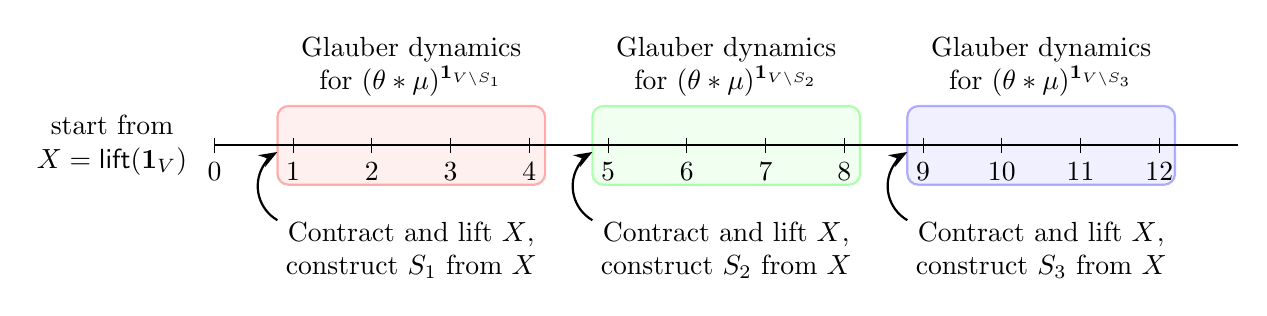
\begin{tikzpicture}
        % Define the background layer
        \pgfdeclarelayer{background}
        \pgfsetlayers{background,main}
        
        % Draw the main line segment from 0 to 13
        \draw[thick] (0, 0) -- (13, 0);
        
        % Draw the ticks and labels
        \foreach \x in {0, 1, ..., 12} {
            \draw (\x, 0.1) -- (\x, -0.1);
            \node[below] at (\x, -0.1) {\x};
        }
        
        % Draw transparent rounded boxes around segments
        \begin{pgfonlayer}{background}
            \filldraw[fill=red!20, draw=red, thick, rounded corners, opacity=0.3] (0.8, -0.5) rectangle (4.2, 0.5);
            \filldraw[fill=green!20, draw=green, thick, rounded corners, opacity=0.3] (4.8, -0.5) rectangle (8.2, 0.5);
            \filldraw[fill=blue!20, draw=blue, thick, rounded corners, opacity=0.3] (8.8, -0.5) rectangle (12.2, 0.5);
        \end{pgfonlayer}
        
        % Add labels on top of the boxes
        \node[above, align=center] at (2.5, 0.5) {Glauber dynamics \\ for $(\theta * \mu)^{\*1_{V \setminus {S_1}}}$};
        \node[above, align=center] at (6.5, 0.5) {Glauber dynamics \\ for $(\theta * \mu)^{\*1_{V \setminus {S_2}}}$};
        \node[above, align=center] at (10.5, 0.5) {Glauber dynamics \\ for $(\theta * \mu)^{\*1_{V \setminus {S_3}}}$};
        
        % Define a vertical shift
        \node[above, align=center] at (-1.3, -0.5) {start from \\ $X=\textsf{lift}(\*1_V)$};
        
        % Add "sample B_i" text and curved arrows
        \def\hshift{-0.2}
        \foreach \i/\x/\textx in {1/1/2.5} {
            \node[below, align=center] at (\textx, -0.85) { Contract and lift $X$, \\construct  $S_{\i}$ from $X$};
            \draw[thick, ->, >=Stealth] (\x+\hshift, -0.95) arc[start angle=240, end angle=120, radius=0.5];
        }
        \foreach \i/\x/\textx in {2/5/6.5, 3/9/10.5} {
            \node[below, align=center] at (\textx, -0.85) {Contract and lift $X$, \\ construct  $S_{\i}$ from $X$};
            \draw[thick, ->, >=Stealth] (\x+\hshift, -0.95) arc[start angle=240, end angle=120, radius=0.5];
        }
    \end{tikzpicture}
    \caption{This figure illustrates the algorithm \(\+A_{\mu}(\theta,T_1,T_2)\) with \(T_1 = 3\) and \(T_2 = 4\). Initially, at time 0, let $X = X^{(0)}_{\text{alg}} = \textsf{lift}(\*1_V)$. Before time 1, the algorithm first contracts $X^{(0)}_{\text{alg}}$ and then lifts it. The algorithm next constructs $S_1 = \{i\in V \mid X_i \neq \star\}$. Then, the algorithm runs Glauber dynamics for the conditional distribution $(\theta * \mu)^{\*1_{V \setminus {S_1}}}$ for $T_2 = 4$ steps to obtain $X^{(t)}_{\text{alg}}$ for $1\leq t \leq 4$. The same procedure is repeated twice to obtain $X= X^{(12)}_{\text{alg}}$.}
    \label{fig:lifted-simulation-algorithm}
    \end{figure}



Using a coupling argument and a simple union bound, we can verify that the algorithm $\+A_\mu(\theta,T_1,T_2)$ produces an accurate sample if $T_1 \geq T_{\text{mix}}^\text{FD}(\mu,\frac{\epsilon}{2})$, which is the mixing time of the field dynamics with an error of $\frac{\epsilon}{2}$, and $T_2 \geq \mixtl(\mu,\theta,\frac{\epsilon}{2T_1})$, which is the mixing time of the Glauber dynamics for the tilted distribution with an error of $\frac{\epsilon}{2T_1}$.
Formally, we have the following lemma. The proof is deferred to \Cref{sec:simu-error}.

\begin{lemma}\label{lem:simu-error}
For any distribution $\mu$ over $\{0,1\}^V$ and any $0< \theta < 1$,  if $T_1 \geq \mixfd(\mu,\frac{\epsilon}{2})$ and $T_2 \geq \mixtl(\mu,\theta,\frac{\epsilon}{2T_1})$, then the output $X = \textsf{contr}(X^{(T_1T_2)}_{\textnormal{alg}})$ of the algorithm $\+A_\mu(\theta,T_1,T_2)$ satisfies
\[\DTV{X}{\mu} \leq \epsilon.\]
\end{lemma}


%Our main technical contribution is the following comparison lemma. 
Let \( (X^{(t)}_{\textnormal{$\mu$-GD}} )_{t \geq 0} \) represent the Glauber dynamics for the distribution \( \mu \) starting from the maximum all-1 state \( X^{(0)}_{\textnormal{$\mu$-GD}} = \*1_V \). 
Our main technical contribution is the following comparison lemma between the Glauber dynamics and the simulation algorithm $\+A_{\mu}(\theta,T_1,T_2)$.
%For any integer \( T \geq 1 \), let \( (P^{\text{GD}}_\mu)^T(\*1_V,\cdot) \) denote the distribution of the output when the Glauber dynamics starts from the maximum all-1 state \( \*1_V \) and makes transitions for $T$ steps.

\begin{lemma} \label{lem:comparison}
Let $\mu$ be a monotone system over $\{0,1\}^V$.
Let \( (X^{(t)}_{\textnormal{$\mu$-GD}} )_{t \geq 0} \) be the Glauber dynamics for $\mu$ starting from $X^{(0)}_{\textnormal{$\mu$-GD}} = \*1_V$.
Let $T_1,T_2 \geq 1$, $\theta \in (0,1)$, and $(X^{(t)}_{\textnormal{alg}})_{t=0}^{T_1T_2}$ be the Markov chain generated by $\+A_{\mu}(\theta,T_1,T_2)$.
For any integer $0 \leq t \leq T_1T_2$, 
\begin{align}\label{eq:comparison-dtv}
    \DTV{X^{(t)}_{\textnormal{$\mu$-GD}}}{\mu} \leq \DTV{\textnormal{\textsf{contr}}(X^{(t)}_{\textnormal{alg}})}{\mu}.
\end{align}
\end{lemma}

%The LHS of \eqref{eq:comparison-dtv} is the total variation distance between $\mu$ and the output of the standard Glauber dynamics.
%The RHS of \eqref{eq:comparison-dtv} is the total variation distance between $\mu$ and the output of the simulation algorithm $\+A_{\mu}(\theta,T_1,T_2)$.
The lemma implies that the $(T_1T_2)$-step Glauber dynamics from the maximum all-1 state returns a more accurate sample than the simulation algorithm $\+A_{\mu}(\theta,T_1,T_2)$. 

\Cref{thm:FD-comparison} is a direct corollary of \Cref{lem:simu-error} and \Cref{lem:comparison}.


\subsection{Stochastic dominance in the lifted space}
We outline the proof of \Cref{lem:comparison}. The algorithm $\+A_{\mu}(\theta,T_1,T_2)$ is a Markov chain over space $\{0,1,\star\}^V$, which generates a sequence of random configurations $X^{(t)}_{\textnormal{alg}}$ for $t=0,1,\ldots,T_1T_2$. In particular, $X^{(0)}_{\textnormal{alg}}=\textsf{lift}(\*1_V)$.
Let $\pi^{(t)}_{\textnormal{alg}}$ denote the distribution of $X^{(t)}_{\textnormal{alg}}$. 

Since the Markov chain is over the space $\{0,1,\star\}^V$, we also lift the distribution $\mu$ to $\{0,1,\star\}^V$. Let $\pi$ denote the distribution of $\textsf{lift}(X)$ for $X \sim \mu$, i.e., 
\begin{align}\label{eq:lift-pi}
    \textsf{lift}(X) \sim \pi \text{ if } X \sim \mu.
\end{align}
By definition, it is easy to see that $\textsf{contr}(Y) \sim \mu$ if $Y \sim \pi$.
Let $\Omega(\mu) \subseteq \{0,1\}^V$ denote the support of $\mu$ and $\Omega(\pi) \subseteq \{0,1,\star\}^V$ denote the support of $\pi$.

Let $P_{\pi\textnormal{-GD}}$ be the transition matrix of the Glauber dynamics on $\pi$. Given the current configuration $X \in \Omega(\pi)$, $P_{\pi\textnormal{-GD}}$ picks a variable $v \in V$ uniformly at random and then resamples $X_v$ from $\pi$ conditional on $X_{V \setminus \{v\}}$. Let $(X^{(t)}_{\pi\textnormal{-GD}})_{t \geq 0}$ denote sequence generated by the Glauber dynamics on $\pi$ starting from $X^{(0)}_{\pi\textnormal{-GD}}= \textsf{lift}(\*1_V)$. Let $\pi^{(t)}_{\textnormal{GD}}$ denote the distribution of $X^{(t)}_{\pi\textnormal{-GD}}$.

A key step in proving \Cref{lem:comparison} is a stochastic dominance relation between distributions $\pi^{(t)}_{\textnormal{alg}}$ and $\pi^{(t)}_{\textnormal{GD}}$.
To state this stochastic dominance result,
we need to extend the partial ordering $\preceq$ on $\{0,1\}^V$ to $\{0,1,\star\}^V$. 
Define the ordering
\begin{align*}
    0 < 1 < \star,
\end{align*}
and the following partial ordering for $X,Y \in \{0,1,\star\}^V$
\begin{align*}
    X \preceq Y \iff \forall v \in V, \,\, X_v \leq Y_v.
\end{align*}
With the above partial ordering, we can use \Cref{def:stochastic-dominance} to define a stochastic dominance relation $\sd$ between distributions over $\{0,1,\star\}^V$.
Note that $\pi^{(0)}_{\textnormal{alg}}=\pi^{(0)}_{\textnormal{GD}}$ at the beginning. The following lemma shows that $\pi^{(t)}_{\textnormal{GD}}$ is always stochastically dominated by $\pi^{(t)}_{\textnormal{alg}}$. 

\begin{lemma}\label{lem:stochastic-dominance}
If $\mu$ is a monotone system, then for any $t \geq 0$, $\pi^{(t)}_{\textnormal{GD}} \sd \pi^{(t)}_{\textnormal{alg}}$.
\end{lemma}

We now explain the intuition behind why \Cref{lem:stochastic-dominance} can be used to prove \Cref{lem:comparison}.
One can verify that $\pi$ is also a monotone system. 
Using the properties of $\pi^{(0)}_{\textnormal{GD}}$ (see \Cref{lem:pi-0-gd}) and the Glauber dynamics, one can verify that $\frac{\pi^{(t)}_{\textnormal{GD}}}{\pi}: \Omega(\pi) \to \mathbb{R}_{\geq 0}$ is an increasing function for any $t \geq 0$.\footnote{See \Cref{sec:preliminaries} for the definition of the function $\frac{\pi^{(t)}_{\textnormal{GD}}}{\pi}$ and the definition of increasing functions.
The statement holds because the Glauber dynamics on $\pi$ is stochastically monotone.
For a formal verification, one can refer to the proof in \Cref{sec:proof-of-the-comparison-result}. The analysis in \Cref{sec:proof-of-the-comparison-result} is for $\mu^{(t)}_{\textnormal{GD}}$ but the same analysis can be applied to $\pi^{(t)}_{\textnormal{GD}}$.
}  Then \Cref{lem:gen-compare} immediately implies that $d_{\text{TV}}(\pi^{(T_1T_2)}_{\textnormal{GD}},\pi) \leq d_{\text{TV}}(\pi^{(T_1T_2)}_{\textnormal{alg}},\pi)$, which means the Glauber dynamics generates a more accurate sample than the simulation algorithm.
This result is similar to the result in \Cref{lem:comparison}. The main difference is that \Cref{lem:comparison} focuses on $\mu$ instead of $\pi$. Specifically, $X^{(T_1T_2)}_{\mu\textnormal{-GD}}$ in \Cref{lem:comparison} is generated by the Glauber dynamics on $\mu$ and \Cref{lem:comparison} considers the contracted configuration $\textsf{contr}(X^{(T_1T_2)}_{\textnormal{alg}})$ instead of $X^{(T_1T_2)}_{\textnormal{alg}}$ itself. 
By definition in~\eqref{eq:lift-pi}, $\mu$ and $\pi$ are closely related. 
This discrepancy can be resolved by analyzing the contracting operation and comparing the Glauber dynamics on $\mu$ to the Glauber dynamics on $\pi$. 
The details of proving \Cref{lem:comparison} assuming \Cref{lem:stochastic-dominance} are deferred to \Cref{sec:comparison-between-original-and-lifted-Glauber-dynamics-1}.







\subsection{Comparison between the Glauber dynamics and the simulation algorithm}

%\todo{discuss why cannot use standard censoring inequality to prove the comparison}

We outline the proof of \Cref{lem:stochastic-dominance}. Note that we cannot directly use the standard censor inequality in \cite{peres2013can} to prove \Cref{lem:stochastic-dominance}.  Here are two reasons: (1) in Line \Cref{item:resample} of $\+A_{\mu}(\theta,T_1,T_2)$, an update on $v$ is ignored if $X_v = \star$. Whether an update at $v$ is ignored \emph{depends} on the current configuration $X$. (2) For vertex $v$ with $X_v \neq \star$, the simulation algorithm and the Glauber dynamics on $\pi$ uses \emph{different} rules to update $X_v$, where the simulation algorithm resamples from the conditional distribution induced by $(\theta * \mu)$ while the Glauber dynamics  resamples from the conditional distribution induced by $\pi$.



We use more general technique in \cite{FillK13}, namely, verifying the comparison inequality relation in \Cref{def:comparison-inequality-relation}.
However, instead of comparing the algorithm with the Glauber dynamics on $\pi$, we compare the algorithm with a \emph{modified Glauber dynamics}. 
We first formulate the simulation algorithm $\+A_{\mu}(\theta,T_1,T_2)$ as a Markov chain over $\{0,1,\star\}^V$, then define the modified Glauber dynamics, and finally compare the algorithm with the modified Glauber dynamics.


\paragraph{Simulation algorithm as a Markov chain}
The algorithm consists of $T_1$ phases, where each phase begins with contracting and lifting operations, and then simulates the Glauber dynamics on $(\theta *\mu)^{\*1_{V \setminus S}}$ for $T_2$ steps (see \Cref{fig:lifted-simulation-algorithm} for an example). Define the following two transition matrices from the simulation algorithm.
\begin{itemize}
    \item $P_{\textnormal{cl}}$: For any $X \in \Omega(\pi)$, transform $X$ to a random $Y = \textsf{lift}(\textsf{contr}(X)) \in \Omega(\pi)$.
    \item $\psim$: For any $X \in \Omega(\pi)$, apply the transitions defined in Line~\ref{item:random-variable} and Line~\ref{item:resample} of the simulation algorithm to transform $X$ to a random $Y \in \Omega(\pi)$.
\end{itemize}
%Let $P_{\textnormal{phase}}$ be the transition matrix of a phase of the simulation algorithm. Since each phase starts with $P_{\textnormal{cl}}$ and repeats $\psim$ for $T_2$ times, we have
%\begin{align}\label{eq:phase-transition}
%    P_{\textnormal{phase}} = P_{\textnormal{cl}} \psim^{T_2}.
%\end{align}
%We remark that $\psim$ is one transition step of simulating the Glauber dynamics on $(\theta *\mu)^{\*1_{V \setminus S}}$. Hence, the transition matrix of one phase is $ P_{\textnormal{cl}} \psim^{T_2}$.
The distribution $\pi^{(t)}_{\textnormal{alg}}$ of $X^{(t)}_{\textnormal{alg}}$ satisfies the following recurrence relation
\begin{align}\label{eq:recurrence-relation-simulation-algorithm}
\pi^{(t+1)}_{\textnormal{alg}} = \pi^{(t)}_{\textnormal{alg}}P_{\textnormal{alg}}^{(t+1)}, \text{ where } P_{\textnormal{alg}}^{(t+1)} = \begin{cases}
    P_{\textnormal{cl}} \psim & \text{if } t \text{ mod } T_2 = 0, \\
    \psim & \text{if } t \text{ mod } T_2 > 0.
\end{cases}
\end{align}
We remark that in $P_{\textnormal{alg}}^{(t+1)}$, $(t+1)$ is the time index of the transition matrix but not the exponent. We always use the bracket notation in upper index to denote the time index.

%The algorithm consists of $T_1$ phases and the transition in each phase is $P_{\textnormal{phase}}$. The overall transition matrix of the algorithm is $P_{\textnormal{phase}}^{T_1} = (P_{\textnormal{cl}} \psim^{T_2})^{T_1}$, i.e. $\pi^{(T_1T_2)}_{\textnormal{alg}} = \pi^{(0)} P_{\textnormal{phase}}^{T_1}$.

\paragraph{A modified Glauber dynamics}
Recall that $P_{\pi\textnormal{-GD}}$ is the transition matrix of the Glauber dynamics on $\pi$. The distribution $\pi^{(t)}_{\textnormal{GD}}$ satisfies the following simple recurrence relation
\begin{align}\label{eq:recurrence-relation-Glauber-dynamics}
    \pi^{(t+1)}_{\textnormal{GD}} = \pi^{(t)}_{\textnormal{GD}} P_{\pi\textnormal{-GD}}.
\end{align}
Note that two recurrences~\eqref{eq:recurrence-relation-simulation-algorithm} and~\eqref{eq:recurrence-relation-Glauber-dynamics} are in the difference forms because $(P_{\textnormal{alg}}^{(t)})_{t \geq 0}$ is time-inhomogeneous but $P_{\pi\textnormal{-GD}}$ is time-homogeneous. To do the comparison, we need to modify the Glauber dynamics. The modification is based on the following property of the chain $P_{\textnormal{cl}}$.
\begin{lemma}\label{lem:many-stationary}
Recall that $\textsf{lift}(\*1_V) \sim \pi^{(0)}_{\textnormal{GD}}$ and $\pi^{(t)}_{\textnormal{GD}} = \pi^{(t-1)}_{\textnormal{GD}}P_{\pi\textnormal{-GD}}$ is the sequence of distributions generated by the Glauber dynamics on $\pi$. Then for any $t \geq 0$,
\begin{align*}
    \pi^{(t)}_{\textnormal{GD}} P_{\textnormal{cl}} = \pi^{(t)}_{\textnormal{GD}}.
\end{align*}
\end{lemma}
The lemma states a very interesting property that contracting-lifting chain $P_{\textnormal{cl}}$ has multiple stationary distributions and \emph{every} $\pi^{(t)}_{\textnormal{GD}}$ is a stationary distribution of $P_{\textnormal{cl}}$. 
The lemma is proved in \Cref{sec:proof-comparison-inequality-relation}.
Using this lemma, we can write the following new recurrence relation for $\pi^{(t)}_{\textnormal{GD}}$
\begin{align}\label{eq:recurrence-relation-Glauber-dynamics-modified}
   \pi^{(t+1)}_{\textnormal{GD}} = \pi^{(t)}_{\textnormal{GD}} P_{\pi\textnormal{-mGD}}^{(t+1)}, \text{ where } P_{\pi\textnormal{-mGD}}^{(t+1)} = \begin{cases}
        P_{\textnormal{cl}} P_{\pi\textnormal{-GD}} & \text{if } t \text{ mod } T_2 = 0, \\
        P_{\pi\textnormal{-GD}} & \text{if } t \text{ mod } T_2 > 0.
    \end{cases}
\end{align}
The above recurrence relation gives a modified time-inhomogeneous Markov chain $(P_{\pi\textnormal{-mGD}}^{(t)})_{t \geq 1}$ for $\pi$. For the transition from time $t$ to time $t+1$, if $t \text{ mod } T_2 = 0$, then the transition matrix is $P_{\textnormal{cl}} P_{\pi\textnormal{-GD}}$; otherwise, the transition matrix is $P_{\pi\textnormal{-GD}}$. 
Thanks to \Cref{lem:many-stationary}, this modified Markov chain generates the same sequence of distributions $(\pi^{(t)}_{\textnormal{GD}})_{t \geq 1}$ as the Glauber dynamics on $\pi$. Now, the good property is that $(P_{\textnormal{alg}}^{(t)})_{t \geq 1}$ and $(P_{\pi\textnormal{-mGD}}^{(t)})_{t \geq 1}$ are in the same form.

\paragraph{Comparison between two Markov chains}
We now apply the general technique in \Cref{sec:preliminaries} to compare the two time-inhomogeneous Markov chains in~\eqref{eq:recurrence-relation-simulation-algorithm} and~\eqref{eq:recurrence-relation-Glauber-dynamics-modified}. 
Recall that by~\eqref{eq:mc-set}, $\+{MC}_\pi$ is the family of Markov chains that are reversible with respect to $\pi$ and stochastically monotone, where the stochastic monotone property is defined in \Cref{def:stochastically-monotone}.
The following properties for $P_{\pi\textnormal{-GD}}$, $P_{\textnormal{cl}}$, and $\psim$ can be verified by their definitions. 
\begin{lemma}\label{lem:properties-of-transition-matrices}
    If $\mu$ is a monotone system, then $P_{\textnormal{cl}} \in \+{MC}_\pi$, $\psim \in \+{MC}_\pi$, and $P_{\pi\textnormal{-GD}} \in \+{MC}_\pi$.
\end{lemma}
The proof of \Cref{lem:properties-of-transition-matrices} is deferred to \Cref{sec:proof-comparison-inequality-relation}. %The above lemma implies $P_{\textnormal{cl}}$ is reversible with respect to $\pi$, which means $\pi$ is also one of the stationary distributions of $P_{\textnormal{cl}}$.

Now, we can use the comparison inequality relation $\mc$ in \Cref{def:comparison-inequality-relation} to compare the two Markov chains.
We prove the following lemma for two transition matrices.
\begin{lemma}\label{lem:phase-comparison}
    If $\mu$ is a monotone system, then $P_{\pi\textnormal{-mGD}}^{(t)} \mc P_{\textnormal{alg}}^{(t)}$ for all $t \geq 1$. 
\end{lemma}
Using \Cref{lem:phase-comparison} and the second property of $\mc$ in \Cref{lem:comparison-inequality-properties}, we have
\begin{align*}
  \forall t \geq 1, \quad P_{\pi\textnormal{-mGD}}^{(1)}P_{\pi\textnormal{-mGD}}^{(2)} \cdots P_{\pi\textnormal{-mGD}}^{(t)} \mc P_{\textnormal{alg}}^{(1)}P_{\textnormal{alg}}^{(2)} \cdots P_{\textnormal{alg}}^{(t)}.  
\end{align*}
Note that $\pi^{(0)}_{\textnormal{GD}} = \pi^{(0)}_{\textnormal{alg}}$ are the distribution of the initial configuration $\textsf{lift}(\*1_V)$. One can verify that $\frac{\pi^{(0)}_{\textnormal{GD}}}{\pi}$ is an increasing function (see \Cref{lem:pi-0-gd}). The definition of $\mc$ in \Cref{def:comparison-inequality-relation} implies \Cref{lem:stochastic-dominance} because $\pi^{(t)}_{\textnormal{GD}} = \pi^{(0)}_{\textnormal{GD}}\prod_{i=1}^t P_{\pi\textnormal{-mGD}}^{(i)}$ and $\pi^{(t)}_{\textnormal{alg}} = \pi^{(0)}_{\textnormal{alg}}\prod_{i=1}^t P_{\textnormal{alg}}^{(i)}$. The formal proof of \Cref{lem:stochastic-dominance} assuming \Cref{lem:phase-comparison} is given in \Cref{sec:proof-stochastic-dominance}.

\begin{remark}
In the above proof, we prove $\pi^{(t)}_{\textnormal{GD}} \sd \pi^{(t)}_{\textnormal{alg}}$ in \Cref{lem:stochastic-dominance} via the comparison between the simulation algorithm and the modified Glauber dynamics in \Cref{lem:phase-comparison}. One might wonder whether we can directly compare the simulation algorithm and the standard Glauber dynamics by showing that $P_{\pi\textnormal{-GD}} \mc P_{\textnormal{alg}}^{(t)}$ for all $t \geq 1$. The answer is no. A counterexample is given in Appendix \ref{sec:counterexample}. Hence, although $\pi^{(t)}_{\textnormal{GD}}$ is defined by the standard Glauber dynamics, when proving the stochastic dominance result for $\pi^{(t)}_{\textnormal{GD}}$, it is \emph{not} necessary to apply the comparison argument to the standard Glauber dynamics. This idea may be of independent interest.
\end{remark}


We give some high-level ideas for the proof of \Cref{lem:phase-comparison}. By comparing~\eqref{eq:recurrence-relation-simulation-algorithm} and~\eqref{eq:recurrence-relation-Glauber-dynamics-modified}, it suffices to show that $P_{\pi\textnormal{-GD}} \mc \psim$. In both $P_{\pi\textnormal{-GD}} $ and $\psim$, the Markov chains first pick a vertex $i \in V$ uniformly at random, and then update the value of $i$ according to their rules. Let $P_{\pi\textnormal{-GD}}^i$ and $\psim^i$ denote the transition matrix conditional on picking vertex $i \in V$. It suffices to show that $P_{\pi\textnormal{-GD}}^i \mc \psim^i$. Fix a distribution $\nu$ such that $\frac{\nu}{\pi}$ is an increasing function. We need to show that $\nu P_{\pi\textnormal{-GD}}^i \sd \nu \psim^i$. One challenge is as follows. Suppose $X \sim \nu$. If $X_i \in \{0,1\}$, then $P_{\pi\textnormal{-GD}}^i$ may update the value of $X_i$ to $\star$, but $\psim$ must update the value of $X_i$ to $\{0,1\}$. Since $\star > 1 > 0$, it seems that $P_{\pi\textnormal{-GD}}^i$ can update $X$ to a larger configuration. However, we can still show $\nu P_{\pi\textnormal{-GD}}^i \sd \nu \psim^i$ by using the fact that $\frac{\nu}{\pi}$ is an increasing function. The intuition is that the increasing property suggests that $X_i$ can also take the value $\star$ with certain probability. In case of $X_i = \star$, $\psim^i$ always keeps the value of $X_i$ as $\star$. Overall, we can show the desired stochastic dominance result. The detailed proof of \Cref{lem:phase-comparison} is given in \Cref{sec:proof-dominance}.


\paragraph{Paper organization}
In \Cref{sec:comparison-between-original-and-lifted-Glauber-dynamics-1}, we first prove \Cref{lem:simu-error} and then prove \Cref{lem:comparison} assuming \Cref{lem:stochastic-dominance}. After that, our task is reduced to proving \Cref{lem:stochastic-dominance}. 
In \Cref{sec:proof-comparison-inequality-relation}, we verify some properties of Markov chains stated in \Cref{lem:many-stationary} and \Cref{lem:properties-of-transition-matrices}. With these properties, we can prove \Cref{lem:stochastic-dominance} assuming \Cref{lem:phase-comparison} in \Cref{sec:proof-stochastic-dominance}. We prove \Cref{lem:phase-comparison} in \Cref{sec:proof-dominance}. This finishes the proof of the main technical result in \Cref{thm:FD-comparison}. Finally,  \Cref{sec:proofs-of-general-results-and-applications} is devoted to proving \Cref{thm:main-comparison} and applications.









\section{Analysis of Glauber dynamics and simulation algorithm}\label{sec:comparison-between-original-and-lifted-Glauber-dynamics-1}
Our main result in \Cref{thm:FD-comparison} is a corollary of \Cref{lem:simu-error} and \Cref{lem:comparison}.
In this section, we first prove \Cref{lem:simu-error} in \Cref{sec:simu-error}.
Then, we prove \Cref{lem:comparison} assuming the stochastic dominance in \Cref{lem:stochastic-dominance} holds.
Specifically, in \Cref{sec:comparison-between-original-and-lifted-Glauber-dynamics-2} and \Cref{sec:analysis-of-contracting-operation}, we give a comparison result of the Glauber dynamics on $\pi$ and $\mu$ and some properties of the lifting and contracting operations, which are used in the proof of \Cref{lem:comparison} in \Cref{sec:proof-of-the-comparison-result}.

\subsection{Correctness of the simulation algorithm}\label{sec:simu-error}
\begin{proof}[Proof of \Cref{lem:simu-error}]
If we can perfectly simulate the field dynamics for $T_1$ steps, then the total variation distance between the output and $\mu$ is at most $\epsilon/2$. In the simulation algorithm, every transition of the field dynamics is simulated by running the Glauber dynamics for $T_2$ steps. By the definition of the mixing time of tilted distributions, for each transition, we can couple the perfect simulation with the simulation algorithm successfully with probability at least $1-\epsilon/(2T_1)$. By a union bound over $T_1$ steps, the total variation distance between the output of the simulation algorithm and the output of the perfect simulation is at most $\epsilon/2$. The lemma follows by the triangle inequality of the total variation distance.
\end{proof}


\subsection{Comparison between Glauber dynamics on \texorpdfstring{$\pi$}{} and \texorpdfstring{$\mu$}{}}\label{sec:comparison-between-original-and-lifted-Glauber-dynamics-2}

We need a middle step to relate the Glauber dynamics on $\pi$ with the Glauber dynamics on $\mu$. 
Recall that $P_{\pi\textnormal{-GD}}$ and $P_{\mu\textnormal{-GD}}$ are the transition matrices of the Glauber dynamics on $\pi$ and $\mu$, respectively. 
Let $(X^{(t)}_{\textnormal{$\pi$-GD}})_{t \geq 0}$ (resp. $(X^{(t)}_{\textnormal{$\mu$-GD}})_{t \geq 0}$) be the sequence generated by the Glauber dynamics for $\pi$ (resp. $\mu$) starting from $X^{(0)}_{\textnormal{$\pi$-GD}} = \textsf{lift}(\*1_V)$ (resp. $X^{(0)}_{\textnormal{$\mu$-GD}} = \*1_V$).
\begin{lemma}\label{lem:comparison-lifted}
    For any integer $t \geq 0$, $X^{(t)}_{\textnormal{$\pi$-GD}}$ and $\textnormal{\textsf{lift}}(X^{(t)}_{\textnormal{$\mu$-GD}})$ are identically distributed, and moreover, $\textnormal{\textsf{contr}}(X^{(t)}_{\textnormal{$\pi$-GD}})$ and $X^{(t)}_{\textnormal{$\mu$-GD}}$ are identically distributed.
\end{lemma}
\begin{proof}

    We first use induction to show that $X^{(t)}_{\textnormal{$\pi$-GD}}$ and $\textnormal{\textsf{lift}}(X^{(t)}_{\textnormal{$\mu$-GD}})$ are identically distributed for any integer $t\geq 0$.
    Let $\mu^{(t)}_{\textnormal{GD}}$ be the distribution of $X^{(t)}_{\mu\textnormal{-GD}}$.
    Recall that $\pi^{(t)}_{\textnormal{GD}}$ denotes the distribution of $X^{(t)}_{\pi\textnormal{-GD}}$.
    When $t=0$, $X^{(0)}_{\pi\textnormal{-GD}}=\textnormal{lift}(\*1_V)=\textnormal{lift}(X^{(0)}_{\mu\textnormal{-GD}})$.

    Assume $X^{(t)}_{\textnormal{$\pi$-GD}}$ and $\textnormal{\textsf{lift}}(X^{(t)}_{\textnormal{$\mu$-GD}})$ are identically distributed for some $t\in \mathbb{N}$. We prove the statement for $t+1$.
    Let $\mu^{(t+1)}_{\textnormal{GD}}\mid_i$ be the distribution of $X^{(t+1)}_{\textnormal{$\mu$-GD}}$ conditional on $i\in V$ is update by the Glauber dynamics. Then we have $\mu^{(t+1)}_{\textnormal{GD}}=\frac{1}{n}\sum_{i\in V}\mu^{(t+1)}_{\textnormal{GD}}\mid_i$. Similarly we can define $\pi^{(t+1)}_{\textnormal{GD}}\mid_i$ and $\pi^{(t+1)}_{\textnormal{GD}}=\frac{1}{n}\sum_{i\in V}\pi^{(t+1)}_{\textnormal{GD}}\mid_i$. Define two functions $C_1,C_\star:\{0,1,\star\}^V \to \mathbb{N}$ that count the number of 1s and $\star$s in a configuration. Formally, for any $\sigma\in \{0,1,\star\}^V$,
    \begin{align}\label{def:c-sigma}
    \begin{split}
    C_1(\sigma)=\abs{\{i\in V\mid\sigma_i=1 \}};\\
    C_\star(\sigma)=\abs{\{i\in V\mid\sigma_i=\star \}}.   
    \end{split}
    \end{align}
    Now, we fix a variable $i \in V$ and fix a configuration $\sigma\in \Omega(\pi) \subseteq \{0,1,\star\}^V$. Define $\tau=\textnormal{contr}(\sigma) \in \Omega(\mu)$. We only need to consider feasible $\sigma,\tau$ because Glauber dynamics stays in feasible space.
    Define $\sigma^{x}$ and $\tau^y$ for $x\in \{0,1,\star\}$ and $y\in\{0,1\}$ by
    \begin{align*}
    &\sigma^x_i=x,\quad \tau^y_i = y;\\
    &\sigma^x_j = \sigma_j,\quad \tau^y_j=\tau_j,\quad \forall j\in V\setminus \{i\}.
    \end{align*}
    In words, $\sigma^x$ and $\tau^y$ are configurations obtained from $\sigma$ and $\tau$ by changing the value of $i$ to $x$ and $y$, respectively.
    We can compute $(\pi^{(t+1)}_{\textnormal{GD}}\mid_i)(\sigma)$ and $(\mu^{(t+1)}_{\textnormal{GD}}\mid_i)(\tau)$ using terms of $\pi^{(t)}_{\textnormal{GD}}$ and $\mu^{(t+1)}_{\textnormal{GD}}$, respectively. By the transition of Glauber dynamics, the value of $i$ is resampled from the conditional distribution, we have
    \begin{align}\label{eq:update-pi-mu}
    \begin{split}
     (\pi^{(t+1)}_{\textnormal{GD}}\mid_i)(\sigma) &= \sum_{x\in \{0,1,\star\}}\pi^{(t)}_{\textnormal{GD}}(\sigma^x)\frac{\pi(\sigma)}{\sum_{z\in \{0,1,\star\}}\pi(\sigma^z)};\\
    (\mu^{(t+1)}_{\textnormal{GD}}\mid_i)(\tau) &= \sum_{y\in \{0,1\}}\mu^{(t)}_{\textnormal{GD}}(\tau^y)\frac{\mu(\tau)}{\sum_{z\in \{0,1\}}\mu(\tau^z)}.   
    \end{split}
    \end{align}
    By definition of $\pi$, $\textsf{lift}(\mu)=\pi$ and $\pi(\sigma) = \mu(\tau)\theta^{C_1(\sigma)}(1-\theta)^{C_\star(\sigma)}$. Hence, $\pi(\sigma^1) + \pi(\sigma^\star)$ equals to $\mu(\tau^1) \theta^{C_1(\sigma^0)}(1-\theta)^{C_\star(\sigma^0)}$. This is because, $\tau^1$ is lifted $\sigma^1$ or $\sigma^\star$ if and only if every $j \neq i$ with $\tau_j = 1$ are lifted correctly.
    It holds that
    \begin{align*}
    \frac{\pi(\sigma)}{\sum_{z\in \{0,1,\star\}}\pi(\sigma^z)} &=\frac{\mu(\tau)\theta^{C_1(\sigma)}(1-\theta)^{C_\star(\sigma)}}{\mu(\tau^0)\theta^{C_1(\sigma^0)}(1-\theta)^{C_\star(\sigma^0)}+\mu(\tau^1)\theta^{C_1(\sigma^0)}(1-\theta)^{C_\star(\sigma^0)}}\\
    &=\frac{\mu(\tau)\theta^{\*1\{\sigma_i=1\}} (1-\theta)^{\*1\{\sigma_i=\star\}}}{\mu(\tau^0)+\mu(\tau^1)},\quad \text{where $\*1\{\cdot\}$ is the indicator function.}
    \end{align*}
    By induction hypothesis, $\textsf{lift}(\mu^{(t)}_{\textnormal{GD}})=\pi^{(t)}_{\textnormal{GD}}$. By the definition of the lifting, we can compute the sum of $\pi^{(t)}_{\textnormal{GD}}(\sigma^z)$ for $z\in \{0,1,\star\}$. Again, the sum of $\pi^{(t)}_{\textnormal{GD}}(\sigma^1) + \pi^{(t)}_{\textnormal{GD}}(\sigma^\star)$ equals to $\mu^{(t)}_{\textnormal{GD}}(\tau^1) \theta^{C_1(\sigma^0)}(1-\theta)^{C_\star(\sigma^0)}$. We have the following equation
    \begin{align*}
    \sum_{z\in \{0,1,\star\}}\pi^{(t)}_{\textnormal{GD}}(\sigma^z)&=\mu^{(t)}_{\textnormal{GD}}(\tau^0)\theta^{C_1(\sigma^0)}(1-\theta)^{C_\star(\sigma^0)}+\mu^{(t)}_{\textnormal{GD}}(\tau^1)\theta^{C_1(\sigma^0)}(1-\theta)^{C_\star(\sigma^0)}\\
    &=(\mu^{(t)}_{\textnormal{GD}}(\tau^0)+\mu^{(t)}_{\textnormal{GD}}(\tau^1))\theta^{C_1(\sigma^0)}(1-\theta)^{C_\star(\sigma^0)}.
    \end{align*}
    Notice that $\theta^{\*1\{\sigma_i=1\}} (1-\theta)^{\*1\{\sigma_i=\star\}}\theta^{C_1(\sigma^0)}(1-\theta)^{C_\star(\sigma^0)}=\theta^{C_1(\sigma)}(1-\theta)^{C_\star(\sigma)}$. Combine above two equations and~\eqref{eq:update-pi-mu}, we have
    \begin{align*}
    (\pi^{(t+1)}_{\textnormal{GD}}\mid_i)(\sigma)&= \frac{\mu(\tau)\theta^{\*1\{\sigma_i=1\}} (1-\theta)^{\*1\{\sigma_i=\star\}}}{\mu(\tau^0)+\mu(\tau^1)} (\mu^{(t)}_{\textnormal{GD}}(\tau^0)+\mu^{(t)}_{\textnormal{GD}}(\tau^1))\theta^{C_1(\sigma^0)}(1-\theta)^{C_\star(\sigma^0)}\\
    &=\theta^{C_1(\sigma)}(1-\theta)^{C_\star(\sigma)}\sum_{x\in \{0,1\}}\mu^{(t)}_{\textnormal{GD}}(\tau^x) \frac{\mu(\tau)}{\sum_{z\in \{0,1\}}\mu(\tau^z)}\\
    &=\theta^{C_1(\sigma)}(1-\theta)^{C_\star(\sigma)} \cdot (\mu^{(t+1)}_{\textnormal{GD}}\mid_i)(\tau).
    \end{align*}
    The above equation can be interpreted as follows: to draw a random sample $\sigma$ from $\pi^{(t+1)}_{\textnormal{GD}}\mid_i$, we first draw a sample $\tau \sim \mu^{(t+1)}_{\textnormal{GD}}\mid_i$, and then apply the lifting operation to $\tau$. We slightly abuse the notation by using $\textsf{lift}(\nu)$ to denote the distribution of $\textsf{lift}(X)$ for $X \sim \nu$. The above equation shows $\pi^{(t+1)}_{\textnormal{GD}}\mid_i = \textsf{lift}(\mu^{(t+1)}_{\textnormal{GD}}\mid_i)$. We have 
    \begin{align*}
    \pi^{(t+1)}_{\textnormal{GD}}=\frac{1}{n}\sum_{i\in V}\pi^{(t+1)}_{\textnormal{GD}}\mid_i = \frac{1}{n} \sum_{i\in V} \textnormal{\textsf{lift}}(\mu^{(t+1)}_{\textnormal{GD}}\mid_i) =\textnormal{\textsf{lift}}(\mu^{(t+1)}_{\textnormal{GD}}),
    \end{align*}
    where the last equality follows from $\mu^{(t+1)}_{\textnormal{GD}} = \frac{1}{n}\sum_{i\in V} \mu^{(t+1)}_{\textnormal{GD}}\mid_i$ and it is straightforward to verify that $\frac{1}{n} \sum_{i\in V} \textnormal{\textsf{lift}}(\mu^{(t+1)}_{\textnormal{GD}}\mid_i) =\textnormal{\textsf{lift}}(\mu^{(t+1)}_{\textnormal{GD}})$. Hence, the above equation shows that $X^{(t+1)}_{\textnormal{$\pi$-GD}} \sim \pi^{(t+1)}_{\textnormal{GD}}$ and $\textnormal{\textsf{lift}}(X^{(t+1)}_{\textnormal{$\mu$-GD}}) \sim \textsf{lift}(\mu^{(t+1)}_{\textnormal{GD}})$ are identically distributed. This proves the induction step.
    
    We next prove the second result. We slightly abuse the notation by using $\textsf{contr}(\nu)$ to denote the distribution of $\textsf{contr}(X)$ for $X \sim \nu$. 
    For any $\tau \in \{0,1\}^V$, it is easy to see $\tau = \textsf{contr}(\textsf{lift}(\tau))$. 
    Hence, for any distribution $\nu$ over $\{0,1\}^V$,  $\nu  =\textsf{contr}(\textsf{lift}(\nu))$. Then for any integer $t\geq 0$, 
    \begin{align*}
    \textnormal{\textsf{contr}}(\pi^{(t)}_{\textnormal{GD}}) = \textnormal{\textsf{contr}}(\textsf{lift}(\mu^{(t)}_{\textnormal{GD}}))= \mu^{(t)}_{\textnormal{GD}}, 
    \end{align*}
    where the first equality holds because of the first result $\pi^{(t)}_{\textnormal{GD}} = \textsf{lift}(\mu^{(t)}_{\textnormal{GD}})$ of the lemma.
    \end{proof}

\subsection{Analysis of contracting operation}\label{sec:analysis-of-contracting-operation}
We also need the following lemma, which shows that the stochastic dominance relation is preserved by the $\textsf{contr}$ operation. The following lemma gives the result for both the lifting and contracting operations. The result for the lifting operation will be used in later sections.
\begin{lemma}\label{lem:lift-and-contr-keep-dominate} 
Let $\nu$ and $\nu'$ be two distributions over $\{0,1\}^V$. Let $\nu_{L}$ be the distribution of $\textsf{lift}(X)$ for $X \sim \nu$ and $\nu_{L}'$ be the distribution of $\textsf{lift}(Y)$ for $Y \sim \nu'$. If $\nu \sd \nu'$, then $\nu_{L} \sd \nu_{L}'$.

Let $\nu$ and $\nu'$ be two distributions over  $\{0,1,\star\}^V$. Let $\nu_{C}$ be the distribution of $\textsf{contr}(X)$ for $X \sim \nu$ and $\nu_{C}'$ the distribution of $\textsf{contr}(Y)$ for $Y \sim \nu'$. If $\nu \sd \nu'$, then $\nu_{C} \sd \nu_{C}'$.
\end{lemma}
\begin{proof}   
Consider two distributions $\nu,\nu'\in \{0,1\}^V$ such that $\nu\preceq\nu'$. By \Cref{def:stochastic-dominance}, there exists a coupling $(X,Y)$ where $X\sim \nu$, $Y\sim \nu'$ such that $X\preceq Y$. We use this $(X,Y)$ to construct a coupling $(P,Q)$ between $\nu_L$ and $\nu_L'$.
For every $i\in V$, $X_i\leq Y_i$. Since the lifting operation lifts each value of $i\in V$ independently, we only need couple the lifting operation on each $i \in V$ such that $\textsf{lift}(X)_i\leq \textsf{lift}(Y)_i$.
If $X_i=Y_i$, then $\textsf{lift}(X)_i=\textsf{lift}(Y)_i$ can be coupled perfectly. If $X_i \neq Y_i$, then the only possible case is $X_i=0$ and $Y_i=1$, and $\textsf{lift}(X)_i=0$, so $\textsf{lift}(X)_i < \textsf{lift}(Y)_i$ because $\textsf{lift}(Y)_i \in \{1,\star\}$.

The contracting operation is a deterministic operation. The second property is easier to verify. 
Consider $\nu,\nu'$ over $\{0,1,\star\}^V$ satisfying $\nu\sd \nu'$.
There exists a coupling $(X,Y)$ where $X\sim \nu$, $Y\sim \nu'$ such that $X\preceq Y$.
We apply the contracting operation to both $X$ and $Y$ to obtain a coupling between $\nu_C$ and $\nu_C'$.
For any $i\in V$, if $X_i=0$, then $\textsf{contr}(X)_i=0\leq \textsf{contr}(Y)_i$. If $X_i=1$ or $X_i=\star$, then $Y_i=1$ or $Y_i=\star$, which implies $\textsf{contr}(X)_i= \textsf{contr}(Y)_i=1$. Hence, there is a coupling between $\nu_C$ and $\nu_C'$ such that $\textsf{contr}(X) \preceq \textsf{contr}(Y)$.
\end{proof}



\subsection{Proof of the comparison result}\label{sec:proof-of-the-comparison-result}
To prove \Cref{lem:comparison}, we need the following lemma.
\begin{lemma}\label{lem:reversible-transition}
Let $P$ be a reversible chain with respect to distribution $\mu$. For any distribution $\nu$, $P \frac{\nu}{\mu} = \frac{\nu P}{\mu}$, where $\frac{\nu}{\mu}$ is a column vector such that $\frac{\nu}{\mu}(\sigma) = \frac{\nu(\sigma)}{\mu(\sigma)}$ and $\nu,\mu$ are row vectors.
\end{lemma}
\begin{proof}
    To verify, for any $x$, we have $(P \frac{\nu}{\mu})(x) = \sum_{y} P(x,y) \frac{\nu(y)}{\mu(y)}$. Since $P$ is reversible, it can be written as $\sum_{y} P(y,x) \frac{\nu(y)}{\mu(x)} = \frac{(\nu P)(x)}{\mu(x)}$.
\end{proof}
Now, we are ready to prove \Cref{lem:comparison}.
\begin{proof}[Proof of \Cref{lem:comparison} assuming \Cref{lem:stochastic-dominance}]
    By \Cref{lem:stochastic-dominance}, $\pi^{(t)}_{\textnormal{GD}} \sd \pi^{(t)}_{\textnormal{alg}}$ for any $t \geq 0$. For any distribution $\nu$, we use $\textsf{contr}(\nu)$ to denote the distribution of $\textsf{contr}(X)$ for $X \sim \nu$. By \Cref{lem:comparison-lifted}, $\textsf{contr}(\pi^{(t)}_{\textnormal{GD}}) = \mu^{(t)}_{\textnormal{GD}}$.
    Using \Cref{lem:lift-and-contr-keep-dominate}, we have $\textsf{contr}(\pi^{(t)}_{\textnormal{GD}}) = \mu^{(t)}_{\textnormal{GD}} \sd \textsf{contr}(\pi^{(t)}_{\textnormal{alg}})$.
   
    We next show that $\frac{\mu^{(t)}_{\textnormal{GD}}}{\mu}: \Omega(\mu) \to \mathbb{R}_{\geq 0}$ is an increasing function.
   Since $\mu$ is a monotone system, by \Cref{def:monotone-system}, the third definition of stochastically monotone chain in \Cref{prop:stochastically-monotone-equivalent}, and the transition of Glauber dynamics, it is straightforward to verify that the Glauber dynamics $P_{\mu\textnormal{-GD}}$ is stochastically monotone. Since $\mu^{(0)}_{\textnormal{GD}}$ takes the maximum configuration $\*1_V$ with probability 1, $\frac{\mu^{(0)}_{\textnormal{GD}}}{\mu}$ is an increasing function. Because $P_{\mu\textnormal{-GD}}$ is reversible with respect to $\mu$, by \Cref{lem:reversible-transition}, for any integer $i\geq 0$,
    $P_{\mu\textnormal{-GD}} \frac{\mu^{(i)}_{\textnormal{GD}}}{\mu} = \frac{\mu^{(i)}_{\textnormal{GD}}P_{\mu\textnormal{-GD}}}{\mu} = \frac{\mu^{(i+1)}_{\textnormal{GD}}}{\mu}$.
    Since $P_{\mu\textnormal{-GD}}$ is stochastically monotone, using \Cref{def:stochastically-monotone}, we verify that $\frac{\mu^{(t)}_{\textnormal{GD}}}{\mu}: \Omega(\mu) \to \mathbb{R}_{\geq 0}$ is an increasing function.

    Note that $X^{(t)}_{\textnormal{alg}}$ in \Cref{lem:comparison} follows the law of $\pi^{(t)}_{\textnormal{alg}}$ and $X^{(t)}_{\textnormal{$\mu$-GD}}$ follows the law of $\mu^{(t)}_{\textnormal{GD}}$.
    With the above two properties, the lemma is proved by \Cref{lem:gen-compare}.
\end{proof}




    


\section{Verification of properties of Markov chains}\label{sec:proof-comparison-inequality-relation}
In this section, we prove the properties of Markov chains stated in \Cref{lem:many-stationary} and \Cref{lem:properties-of-transition-matrices}.

\Cref{lem:many-stationary} is a straightforward consequence of \Cref{lem:comparison-lifted}.
\begin{proof}[Proof of \Cref{lem:many-stationary}]
The Markov chain $P_{\textnormal{cl}}$ can be decomposed as $P_CP_L$. Using \Cref{lem:comparison-lifted}, $\pi^{(t)}_{\textnormal{GD}} P_C = \mu^{(t)}_{\textnormal{GD}}$ and $\mu^{(t)}_{\textnormal{GD}} P_L = \pi^{(t)}_{\textnormal{GD}}$. Therefore, $\pi^{(t)}_{\textnormal{GD}} P_{\textnormal{cl}} = \pi^{(t)}_{\textnormal{GD}}$, where $\mu^{(t)}_{\textnormal{GD}}$ is distribution of $X^{(t)}_{\mu\textnormal{-GD}}$ in \Cref{lem:comparison-lifted}, which is the sequence of distributions generated by Glauber dynamics on $\mu$ starting from $\*1_V$. This proves the lemma.

The above proof suggests that for any distribution $\mu$ over $\Omega(\mu)$, $\mu P_{\textnormal{L}}$ over $\Omega(\pi)$ is a stationary distribution of the chain $P_{\textnormal{cl}}$. This is because $\mu P_{\textnormal{L}}P_{\textnormal{cl}} = \mu P_{\textnormal{L}}P_{\textnormal{C}}P_{\textnormal{L}} = \mu P_{\textnormal{L}}$ as $P_{\textnormal{L}}P_{\textnormal{C}} = I$.
\end{proof}




To prove \Cref{lem:properties-of-transition-matrices}, we need to show that Markov chains $P_{\pi\textnormal{-GD}}$, $P_{\textnormal{cl}}$ and $\psim$ are stochastically monotone and reversible, which are proved in \Cref{sec:proof-stochastically-monotone} and \Cref{sec:proof-reversible}.



\subsection{Stochastic monotonicity of Markov chains}\label{sec:proof-stochastically-monotone}
We first show that $\pi$ is a monotone system over $\Omega(\pi) \subseteq \{0,1,\star\}^V$.
We extend the definition of a monotone system in \Cref{def:monotone-system} to the case that the distribution is over $\{0,1,\star\}^V$. We say the lifted distribution $\pi$ is a monotone system if for any $i \in V$, for any feasible and comparable configurations $\sigma\preceq \tau$ with $\sigma,\tau \in \{0,1,\star\}^{V \setminus \{i\}}$, the conditional distribution $\pi^{\sigma}_i$ is stochastically dominated by $\pi^{\tau}_i$, which means there exists a coupling $(x,y)$ of $\pi^{\sigma}_i$ and $\pi^{\tau}_i$ such that $x\leq y$ with probability~1, where we use the ordering $0 < 1 < \star$.
By the monotonicity of the distribution $\mu$, we have the following property for the lifted distribution $\pi$, which implies that the Glauber dynamics $P_{\pi\textnormal{-GD}}$ is stochastically monotone.
\begin{lemma}\label{lem:monotone-pi}
If $\mu$ is a monotone system, then $\pi$ is also a monotone system. This implies the Glauber dynamics $P_{\pi\textnormal{-GD}}$ on $\pi$ is stochastically monotone.
\end{lemma}
\begin{proof}
Given any configuration $\sigma\in \Omega(\pi)$ and any $i \in V$, for any $x\in \{0,1,\star\}$, let $\sigma^x$ be the configuration obtained from $\sigma$ by setting $\sigma_i=x$.
The conditional distribution of $\pi$ is
\begin{align*}
\pi^{\sigma_{V \setminus \{i\}}}_i(0)=\frac{\pi(\sigma^0)}{\pi(\sigma^0)+\pi(\sigma^\star)+\pi(\sigma^1)}.
\end{align*}
Note that $\pi(\sigma^0) = \mu(\textsf{Contr}(\sigma^0)) \theta^{C_1(\sigma^0)}(1-\theta)^{C_\star(\sigma^0)}$, where $C_1$ and $C_\star$ are defined in~\eqref{def:c-sigma}, and $\pi(\sigma^\star) + \pi(\sigma^1) = \mu(\textsf{Contr}(\sigma^1)) \theta^{C_1(\sigma^1)-1}(1-\theta)^{C_\star(\sigma^1)}$. The second equation holds because to obtain $\sigma^1$ or $\sigma^\star$ from $\pi$, we first need to sample $X \sim \mu$ such that $X = \textsf{Contr}(\sigma^1)$, and for any $j \neq i$ with $X_j = 1$, if $\sigma_j = 1$, we need to keep the value of $X_j$ in the lifting operation, which happens with probability $\theta$; if $\sigma_j = \star$, we need to lift the value of $X_j$ to $\star$ in the lifting operation, which happens with probability $1-\theta$. Combining these two equations, we have 
\begin{align}\label{eq:pi-0-i}
    \pi^{\sigma_{V \setminus \{i\}}}_i(0) = \frac{\mu(\textsf{Contr}(\sigma^0))}{\mu(\textsf{Contr}(\sigma^0))+\mu(\textsf{Contr}(\sigma^1))}.
\end{align}
Similarly, we have 
\begin{align}\label{eq:pi-1-i}
    \pi^{\sigma_{V \setminus \{i\}}}_i(1) = \frac{\theta \mu(\textsf{Contr}(\sigma^1))}{\mu(\textsf{Contr}(\sigma^0))+\mu(\textsf{Contr}(\sigma^1))},\quad \pi^{\sigma_{V \setminus \{i\}}}_i(\star) =  \frac{(1-\theta)\mu(\textsf{Contr}(\sigma^1))}{\mu(\textsf{Contr}(\sigma^0))+\mu(\textsf{Contr}(\sigma^1))}.
\end{align}

Hence, we can use the following process to sample from the distribution $\pi^{\sigma_{V \setminus \{i\}}}_i$: (1) Sample $x \sim  \mu_i^{\textsf{Contr}(\sigma)_{V \setminus \{i\}}}$; (2) If $x_i = 0$, then output $0$; (3) If $x_i = 1$, then output $1$ with probability $\theta$ and output $\star$ with the rest probability $1-\theta$.

For $\sigma, \tau \in \Omega(\pi)$ such that $\sigma\preceq \tau$, construct the following coupling of $\pi^{\sigma_{V \setminus \{i\}}}_i$ and $\pi^{\tau_{V \setminus \{i\}}}_i$.
\begin{enumerate}
    \item Since $\sigma \preceq \tau$, we have $\textsf{Contr}(\sigma) \preceq \textsf{Contr}(\tau)$. Since $\mu$ is a monotone system, we can sample $(x,y)$ from the coupling of $\mu^{\textsf{Contr}(\sigma)_{V \setminus \{i\}}}_i$ and $\mu^{\textsf{Contr}(\tau)_{V \setminus \{i\}}}_i$ such that  $x \leq y$.
    \item If $x= 0$, then keep $x = 0$. Randomly lift the value of $y$ if $y = 1$. In this case, $0 = x \leq y$.
    \item If $x = 1$, then $1 = y \geq x = 1$. Use the perfect coupling to lift both $x$ and $y$, so that $x = y$.
\end{enumerate}
The above coupling of $\pi^{\sigma_{V \setminus \{i\}}}_i$ and $\pi^{\tau_{V \setminus \{i\}}}_i$ satisfies that $x \leq y$ with probability~1. Therefore, $\pi^{\sigma_{V \setminus \{i\}}}_i \preceq \pi^{\tau_{V \setminus \{i\}}}_i$ for any $i \in V$ and any  $\sigma \preceq \tau$. 

Using the third definition in \Cref{prop:stochastically-monotone-equivalent}, it is straightforward to show that the Glauber dynamics $P_{\pi\textnormal{-GD}}$ is stochastically monotone.
\end{proof}

Next, we show that the chain $\psim$ is stochastically monotone. We need the following lemma, which says the monotone property is preserved by tilted distributions.
\begin{lemma}\label{lem:monotone-pi-sgd}
If $\mu$ over $\{0,1\}^V$ is a monotone system, then for any $\theta > 0$, the tilted distribution $(\theta * \mu)$ is a monotone system.
\end{lemma}
\begin{proof}
Fix two feasible configurations $\sigma$ and $\tau$ in $\Omega(\mu) = \Omega(\theta * \mu)$ such that $\sigma\preceq \tau$. We need to show that for any $i \in V$, $(\theta * \mu)^{\sigma_{V \setminus \{i\}}}_i(1) \leq (\theta * \mu)^{\tau_{V \setminus \{i\}}}_i(1)$. A simple calculation shows that
\begin{align}\label{eq:theta-mu-monotone}
    (\theta * \mu)^{\sigma_{V \setminus \{i\}}}_i(1) = \frac{\theta \mu^{\sigma_{V \setminus \{i\}}}_i(1)}{\theta \mu^{\sigma_{V \setminus \{i\}}}_i(1) + \mu^{\sigma_{V \setminus \{i\}}}_i(0)} \text{ and } (\theta * \mu)^{\tau_{V \setminus \{i\}}}_i(1) = \frac{\theta \mu^{\tau_{V \setminus \{i\}}}_i(1)}{\theta \mu^{\tau_{V \setminus \{i\}}}_i(1) + \mu^{\tau_{V \setminus \{i\}}}_i(0)}.
\end{align}
The lemma follows from $\mu^{\sigma_{V \setminus \{i\}}}_i(1) \leq \mu^{\tau_{V \setminus \{i\}}}_i(1)$ by the monotonicity of $\mu$.
\end{proof}

\begin{lemma}\label{lem:monotone-sgd}
If $\mu$ is a monotone system, then the chain $\psim$ is stochastically monotone.
\end{lemma}
\begin{proof}
We use the third definition in \Cref{prop:stochastically-monotone-equivalent} to prove the result. Fix two feasible and comparable configurations $\sigma$ and $\tau$ in $\Omega(\pi) \subseteq \{0,1,\star\}^V$ such that $\sigma\preceq \tau$. We need to show that $\psim(\sigma,\cdot) \sd \psim(\tau,\cdot)$. The Markov chain $\psim$ picks vertex $i$ uniformly at random and then updates the value of $i$. We show that stochastic dominance holds conditional on any $i \in V$ is picked by the Markov chain. 
Since $\sigma\preceq \tau$, we have following cases.

Case $\tau_i = \star$. In this case, $\psim$ must keep the value of $\tau_i = \star$. Since $\star > 1 > 0$ is the largest value, it is straightforward to verify the stochastic dominance result.
 
Case $\tau_i \in \{0,1\}$. In this case, it must hold that $\sigma_i \in \{0,1\}$. The Markov chain $\psim$ resamples $\tau_i$ from the distribution $(\theta * \mu)^{\tau'}_i$, where $\tau'$ is a configuration over $V \setminus \{i\}$ such that $\tau' = \textsf{Contr}(\tau)_{V \setminus \{i\}}$. Similarly, $\psim$ resamples $\sigma_i$ from the distribution $(\theta * \mu)^{\sigma'}_i$, where $\sigma'$ is a configuration over $V \setminus \{i\}$ such that $\sigma' = \textsf{Contr}(\sigma)_{V \setminus \{i\}}$. Since $\sigma \preceq \tau$, by the definition of contracting operation, we have $\sigma' \preceq \tau'$. We know that $(\theta * \mu)$ is a monotone system by \Cref{lem:monotone-pi-sgd}. Therefore, we have $(\theta * \mu)^{\sigma'}_i \sd(\theta * \mu)^{\tau'}_i$.
\end{proof}

\begin{lemma}\label{lem:monotone-pcl}
The chain $P_{\textnormal{cl}}$ is always stochastically monotone.
\end{lemma}
\begin{proof}
The chain $P_{\textnormal{cl}}$ can be viewed as a Markov chain defined over the whole space $\{0,1,\star\}^V$. We use the second definition in \Cref{prop:stochastically-monotone-equivalent} to prove the result. For two distributions $\nu$ and $\nu'$ over $\{0,1,\star\}^V$ such that $\nu \sd \nu'$, we need to show that for any $\nu \psim \sd \nu' \psim$. This result is a straightforward consequence of \Cref{lem:lift-and-contr-keep-dominate}.
\end{proof}


\subsection{Reversibility of Markov chains}\label{sec:proof-reversible}
\begin{lemma}\label{lem:reversible-pcl}
All Markov chains $P_{\pi\textnormal{-GD}}$, $P_{\textnormal{cl}}$ and $\psim$ are reversible with respect to $\pi$.
\end{lemma}
\begin{proof}
The reversibility of $P_{\pi\textnormal{-GD}}$ is well-known. We prove the reversibility of $P_{\textnormal{cl}}$ and $\psim$ with respect to $\pi$.
Note that starting from any feasible configuration, the two chains always stay in feasible space $\Omega(\pi)$. We only need to prove the detailed balance equation for any pair of configurations in $\Omega(\pi)$.

Fix two configurations $\sigma$ and $\tau$ in $\Omega(\pi)$. For $P_{\textnormal{cl}}$, we need to show that 
\[\pi(\sigma) P_{\textnormal{cl}}(\sigma,\tau) = \pi(\tau) P_{\textnormal{cl}}(\tau,\sigma).\]
By the definition of the contracting and lifting operation, if $\{v \in V \mid \sigma_v = 0\} \neq \{v \in V \mid \tau_v = 0\}$, then $P_{\textnormal{cl}}(\sigma,\tau) = P_{\textnormal{cl}}(\tau,\sigma) = 0$. Assume the two sets are the same, which means $\textsf{Contr}(\sigma) = \textsf{Contr}(\tau)$. Recall that $C_1,C_\star$ in \eqref{def:c-sigma} count the number of $1$s and $\star$s in the configuration. We have $P_{\textnormal{cl}}(\sigma,\tau) = \theta^{C_1(\tau)}(1 - \theta)^{C_\star(\tau)}$ and $P_{\textnormal{cl}}(\tau,\sigma) = \theta^{C_1(\sigma)}(1 - \theta)^{C_\star(\sigma)}$. The reversibility is proved by noting that $\pi(\sigma) = \mu(\textsf{Contr}(\sigma))\theta^{C_1(\sigma)}(1 - \theta)^{C_\star(\sigma)}$ and $\pi(\tau) = \mu(\textsf{Contr}(\tau))\theta^{C_1(\tau)}(1 - \theta)^{C_\star(\tau)}$.

For $\psim$, we need to show the following detailed balance equation.
\[\pi(\sigma) \psim(\sigma,\tau) = \pi(\tau) \psim(\tau,\sigma).\]
If $\sigma = \tau$, then the equality holds trivially. Assume $\sigma \neq \tau$. By the definition of $\psim$, we only need to consider the case where there exists exactly one $i \in V$ such that $\sigma_i \neq \tau_i$ and the two values are $0$ or $1$. Otherwise, the transition probabilities on both sides are 0. Assume $\sigma_i = 0$ and $\tau_i = 1$. Let $\rho = \sigma_{V \setminus \{i\}} = \tau_{V \setminus \{i\}}$. The above equality is equivalent to 
\[\pi^\rho_i(0) \psim(\sigma,\tau) = \pi^\rho_i(1) \psim(\tau,\sigma).\]
Using~\eqref{eq:pi-0-i} and~\eqref{eq:pi-1-i}, we have
\begin{align}\label{eq:pi-rho-i}
    \pi^{\rho}_i(0) = \frac{\mu(\textsf{Contr}(\sigma))}{\mu(\textsf{Contr}(\sigma))+\mu(\textsf{Contr}(\tau))}, \quad  \pi^{\rho}_i(1) = \frac{\theta \mu(\textsf{Contr}(\tau))}{\mu(\textsf{Contr}(\sigma))+\mu(\textsf{Contr}(\tau))},
\end{align}
By the definition of the Markov chain $\psim$, using~\eqref{eq:theta-mu-monotone} and a simple normalization, we have 
\begin{align}\label{eq:psim-rho}
    \begin{split}
        \psim(\sigma,\tau) &= (\theta * \mu)^{\textsf{Contr}(\sigma)_{V \setminus \{i\}}}_{i}(1) =\frac{\theta \mu(\textsf{Contr}(\tau))}{\theta \mu(\textsf{Contr}(\tau))+ \mu(\textsf{Contr}(\sigma))},\\
        \psim(\tau,\sigma) &= (\theta * \mu)^{\textsf{Contr}(\tau)_{V \setminus \{i\}}}_{i}(0) =\frac{\mu(\textsf{Contr}(\sigma))}{\theta \mu(\textsf{Contr}(\tau))+ \mu(\textsf{Contr}(\sigma))}.
    \end{split}
\end{align}
Combining~\eqref{eq:pi-rho-i} and~\eqref{eq:psim-rho} proves the detailed balance equation.
\end{proof}




\section{Proof of stochastic dominance}\label{sec:proof-stochastic-dominance}
%In \Cref{sec:proof-comparison-inequality-relation}, we proved \Cref{lem:many-stationary} and \Cref{lem:properties-of-transition-matrices}. 
In this section, we assume that  \Cref{lem:phase-comparison} holds and prove the stochastic dominance result in \Cref{lem:stochastic-dominance}. The proof of \Cref{lem:phase-comparison} is deferred to \Cref{sec:proof-dominance}. 

Recall that $\pi^{(0)}_{\textnormal{GD}}$ is the distribution of $\textsf{lift}(\*1_V)$. The following lemma gives the property that $\pi^{(0)}_{\textnormal{GD}}$ is increasing, which will be used in the proof of \Cref{lem:stochastic-dominance}.

\begin{lemma}\label{lem:pi-0-gd}
The function $\frac{\pi^{(0)}_{\textnormal{GD}}}{\pi}$ is an increasing function.
\end{lemma}
\begin{proof}
    Recall that two functions $C_1$ and $C_\star$ are defined in~\eqref{def:c-sigma}. 
    \begin{align*}
     \forall \sigma\in \{0,1,\star\}^V,\quad   \pi^{(0)}_{\textnormal{GD}}(\sigma) = \begin{cases}
            0, & \text{if } \exists i\in V, \sigma_i=0;\\
            \theta^{C_1(\sigma)}(1-\theta)^{C_\star(\sigma)}, & \text{otherwise}.
        \end{cases}  
    \end{align*}
    Consider two configurations $\sigma$ and $\tau$ such that $\sigma\preceq \tau$. We show that $\frac{\pi^{(0)}_{\textnormal{GD}}(\sigma)}{\pi(\sigma)}\leq \frac{\pi^{(0)}_{\textnormal{GD}}(\tau)}{\pi(\tau)}$. By definition of $\preceq$, $\sigma_i\leq\tau_i$ for all $i\in V$. If there exists an $i\in V$ such that $\sigma_i=0$,
    \begin{align*}
    \frac{\pi^{(0)}(\sigma)}{\pi(\sigma)}=0\leq \frac{\pi^{(0)}(\tau)}{\pi(\tau)}.
    \end{align*}
    We only need to consider the case where $1\leq \sigma_i\leq \tau_i$ for all $i\in V$.
    By the definition of $\pi$, for these configurations, $\pi(\sigma)=\mu(\*1_V)\theta^{C_1(\sigma)}(1-\theta)^{C_\star(\sigma)}$. We have
    \begin{align*}
    \frac{\pi^{(0)}_{\textnormal{GD}}(\sigma)}{\pi(\sigma)}=\frac{\theta^{C_1(\sigma)}(1-\theta)^{C_\star(\sigma)}}{\mu(\*1_V)\theta^{C_1(\sigma)}(1-\theta)^{C_\star(\sigma)}}=\frac{1}{\mu(\*1_V)}=\frac{\pi^{(0)}_{\textnormal{GD}}(\tau)}{\pi(\tau)}.
    \end{align*}
    Therefore, $\frac{\pi^{(0)}_{\textnormal{GD}}}{\pi}$ is an increasing function. 
\end{proof}



Now, we are ready to prove \Cref{lem:stochastic-dominance}.

\begin{proof}[Proof of \Cref{lem:stochastic-dominance} assuming \Cref{lem:phase-comparison}]
    Recall that $\pi^{(0)}_{\textnormal{GD}} = \pi^{(0)}_{\textnormal{alg}}$ is the distribution of the initial configuration $\textsf{lift}(\*1_V)$.
Recall that $\pi^{(t)}_{\textnormal{alg}}$ are defined by the recurrence relation \eqref{eq:recurrence-relation-simulation-algorithm}. Recall that $\pi^{(t)}_{\textnormal{GD}}$ is defined by $\pi^{(t)}_{\textnormal{GD}} = \pi^{(t-1)}_{\textnormal{GD}}P_{\pi\textnormal{-GD}}$. By \Cref{lem:many-stationary}, $\pi^{(t)}_{\textnormal{GD}}$ also satisfies the recurrence relation given in \eqref{eq:recurrence-relation-Glauber-dynamics-modified}. Hence, we can write 
\begin{align}\label{eq:recurrence-relation-Glauber-dynamics-modified-2}
\pi^{(t)}_{\textnormal{GD}} = \pi^{(0)}_{\textnormal{GD}}\prod_{i=1}^t P_{\pi\textnormal{-mGD}}^{(i)} \quad\text{and}\quad \pi^{(t)}_{\textnormal{alg}} = \pi^{(0)}_{\textnormal{alg}}\prod_{i=1}^t P_{\textnormal{alg}}^{(i)}. 
\end{align}
Using \Cref{lem:phase-comparison} and the second property of $\mc$ in \Cref{lem:comparison-inequality-properties}, we have
\begin{align*}
  \forall t \geq 1, \quad \prod_{i=1}^t P_{\pi\textnormal{-mGD}}^{(i)}  \mc \prod_{i=1}^t P_{\textnormal{alg}}^{(i)}.  
\end{align*}
By \Cref{lem:pi-0-gd}, $\frac{\pi^{(0)}_{\textnormal{GD}}}{\pi} = \frac{\pi^{(0)}_{\textnormal{alg}}}{\pi}$ is an increasing function. By the definition of $\mc$ in \Cref{def:comparison-inequality-relation} and~\eqref{eq:recurrence-relation-Glauber-dynamics-modified-2}, we have $\pi^{(t)}_{\textnormal{GD}} \sd \pi^{(t)}_{\textnormal{alg}}$.
\end{proof}






\section{Proof of the comparison inequality relation}\label{sec:proof-dominance}



In this section, we prove \Cref{lem:phase-comparison}. Fix a time $t$, there are two cases (1) $P^{(t)}_{\textnormal{alg}} = \psim$ and $P^{(t)}_{\pi\textnormal{-mGD}} = P_{\pi\textnormal{-GD}}$; (2) $P^{(t)}_{\textnormal{alg}} = P_{\textnormal{cl}}\psim$ and $P^{(t)}_{\pi\textnormal{-mGD}} = P_{\textnormal{cl}}P_{\pi\textnormal{-GD}}$. Since $P_{\textnormal{cl}} \mc P_{\textnormal{cl}}$, by the second property of $\mc$ in \Cref{lem:comparison-inequality-properties}, to show that $P^{(t)}_{\pi\textnormal{-GD}} \mc P^{(t)}_{\textnormal{alg}}$, we only need to show that $P_{\pi\textnormal{-GD}} \mc \psim$. For any vertex $i \in V$, let $\psim^i$ denote the transition in $\psim$ conditioned on that the vertex $i \in V$ is being selected, and let $P^i_{\pi\textnormal{-GD}}$ denote the transition in $P_{\pi\textnormal{-GD}}$ conditioned on that the vertex $i \in V$ is being selected. It holds that 
\begin{align*}
   \psim = \frac{1}{n}\sum_{i\in V} \psim^i, \quad P_{\pi\textnormal{-GD}} = \frac{1}{n}\sum_{i\in V} P^i_{\pi\textnormal{-GD}}.
\end{align*}
Using the first property of $\mc$ in \Cref{lem:comparison-inequality-properties}, to prove that $P_{\pi\textnormal{-GD}} \mc \psim$, it suffices to show that for any vertex $i \in V$, $P^i_{\pi\textnormal{-GD}} \mc \psim^i$. Hence, the proof of \Cref{lem:phase-comparison} can be reduced to proving the following lemma.
\begin{lemma}\label{lem:phase-comparison-single-vertex}
For any vertex $i \in V$, $P^i_{\pi\textnormal{-GD}} \mc \psim^i$.
\end{lemma}
\begin{proof}
%Let $P_\text{alg}^i$ denote the transition in $P_\text{alg}$ conditioned on the vertex $i \in V$ is being selected in the first step. Let $P^i_{\pi\textnormal{-GD}}$ denote the transition in $P_{\pi\textnormal{-GD}}$ conditioned on the vertex $i \in V$ is being selected by the Glauber dynamics. We view both $P_\text{alg}^i$ and $P^i_{\pi\textnormal{-GD}}$ as the transition matrices in space $\{0,1,\star\}^V$. We have 
Recall that $\Omega(\pi)$ is the support of $\pi$.
Fix a vertex $i \in V$. 
By the definition of $\mc$, we need to show that for any distribution $\nu$ over $\Omega(\pi)$ such that the function $\frac{\nu}{\pi}:\Omega(\pi) \to \mathbb{R}_{\geq 0}$ is increasing, $\nu P^i_{\pi\textnormal{-GD}} \preceq_{\text{sd}} \nu \psim^i$. Define two distributions
\begin{align*}
\nug = \nu P_{\pi\textnormal{-GD}}, \quad \nus = \nu \psim^i.
\end{align*}
To show $\nug \sd \nus$, it suffices to show that for any increasing function $f:\{0,1,\star\}^V\to \mathbb{R}_{\geq 0}$\footnote{To prove the stochastic dominance, we only need to consider the increasing functions $f$ that are supported on $\Omega(\pi)$. Here, we consider a more general class of functions over $\{0,1,\star\}^V$, which is sufficient for the proof. The benefit is that in the rest of the proof (such as~\eqref{eq:exp-nu-i-1}), $f(\sigma)$ is well-defined for any $\sigma \in \{0,1,\star\}^V$.},
\begin{align}\label{eq:ineq-i-each}
    \E[\nug]{f}\leq \E[\nus]{f}.
\end{align}






For $x\in \{0,1,\star\}$ and a configuration $\sigma\in \{0,1,\star\}^V$, define $\sigma^x$ to be a configuration by changing the value of $\sigma_i$ to $x$, and keeping other values the same as $\sigma$. Formally,
\begin{align*}
    \begin{cases}
&\sigma^x_{i} = x,\\
&\sigma^x_j = \sigma_j,\quad \forall j\in V\setminus \{i\}.   
\end{cases}
\end{align*}





By the definition of $P^i_{s\textnormal{-GD}}$,
we have the following relation between $\nus$ and $\nu$. For any $\sigma\in \{0,1,\star\}^V$ such that $\sigma_{V \setminus \{i\}}$ is a feasible partial configuration on $V \setminus \{i\}$, it holds that
\begin{align}\label{eq:recur-alg}
\begin{split}
&\nus(\sigma^{\star}) = \nu(\sigma^{\star}),\\
&\nus(\sigma^1)=(\nu(\sigma^0)+\nu(\sigma^1))\frac{\theta \mu(\textsf{contr}(\sigma^1))}{\mu(\textsf{contr}(\sigma^0))+\theta \mu(\textsf{contr}(\sigma^1))},\\
&\nus(\sigma^0)=(\nu(\sigma^0)+\nu(\sigma^1))\frac{\mu(\textsf{contr}(\sigma^0))}{\mu(\textsf{contr}(\sigma^0))+\theta \mu(\textsf{contr}(\sigma^1))}.
\end{split}
\end{align}
We explain the above three equations in the following way. Let $X \sim \nu$ and $X'$ be the configuration obtained by applying $P^i_{s\textnormal{-GD}}$ to $X$.
The first equation is because $X'_i = \star$ if and only if $X_i = \star$.
For the second and the third equations, if $X' = \sigma^0$ or $\sigma^1$, then $X_i = 0$ or $1$ and $X'_i$ is resampled from $(\theta * \mu)_i^\tau$ for $\tau = \textsf{contr}(\sigma)_{V \setminus \{i\}}$. Note that in the contracting operation, the value $\star$ is mapped to $1$. We can calculate
\begin{align}\label{eq:recur-alg-2}
    (\theta * \mu)_i^{\tau}(1) = \frac{(\theta * \mu)(\textsf{contr}(\sigma^1))}{(\theta * \mu)(\textsf{contr}(\sigma^0))+(\theta * \mu)(\textsf{contr}(\sigma^1))}.
\end{align}
Let $\Vert \sigma \Vert_1$ be the number of $1$s in $\sigma$. Note that $\Vert \textsf{contr}(\sigma^1) \Vert_1 = \Vert \textsf{contr}(\sigma^0) \Vert_1 + 1$. Hence, the second and the third equations in~\eqref{eq:recur-alg} hold by~\eqref{eq:recur-alg-2}.

Consider the expectation $\E[\nus]{f}$. It can be written as
\begin{align}\label{eq:exp-nu-i-1}
\E[\nus]{f}=\sum_{\sigma\in \{0,1,\star\}^V} \nus(\sigma)f(\sigma)=\frac{1}{3} \sum_{\sigma\in \{0,1,\star\}^V}\sum_{x\in\{0,1,\star\} } \nus(\sigma^x)f(\sigma^x). 
\end{align}
The last equation holds because we enumerate all full configurations $\sigma \in \{0,1,\star\}^V$. For $\sigma = \sigma^{x}$ where $x\in \{0,1,\star\}$, the second sum over $x$ is the same. Hence, any $\sigma \in \{0,1,\star\}^V$ is counted $3$ times in the last summation.
Note that for the last sum over $\sigma$, we only need to consider $\sigma$'s that $\sigma_{V \setminus \{i\}}$ is a feasible partial configuration on $V \setminus \{i\}$. Otherwise, $\pi(\sigma^x) = 0$ for all $x\in \{0,1,\star\}$. Since Markov chain $P^i_{s\textnormal{-GD}}$ always stays in feasible space, $\nus(\sigma^x) = 0$ for all $x$.
Fix an arbitrary one of such configurations $\sigma \in \{0,1,\star\}^V$. Consider the term $\sum_{x\in \{0,1,\star\}} \nus(\sigma^x)f(\sigma^x)$ in~\eqref{eq:exp-nu-i-1}.
Using the relation in~\eqref{eq:recur-alg}, we have
\begin{align}\label{eq:exp-nu-i}
&\sum_{x\in \{0,1,\star\}} \nus(\sigma^x)f(\sigma^x)= \nu(\sigma^\star) f(\sigma^\star)+(\nu(\sigma^0)+\nu(\sigma^1))\frac{\theta \mu(\textsf{contr}(\sigma^1))f(\sigma^1)}{\mu(\textsf{contr}(\sigma^0))+\theta \mu(\textsf{contr}(\sigma^1))}\notag\\
&\qquad\qquad\qquad\qquad\qquad+(\nu(\sigma^0)+\nu(\sigma^1))\frac{ \mu(\textsf{contr}(\sigma^0))f(\sigma^0)}{\mu(\textsf{contr}(\sigma^0))+\theta \mu(\textsf{contr}(\sigma^1))} \notag\\
&=\nu(\sigma^\star) f(\sigma^\star)+(\nu(\sigma^0)+\nu(\sigma^1))\frac{ \mu(\textsf{contr}(\sigma^0))f(\sigma^0)+\theta \mu(\textsf{contr}(\sigma^1))f(\sigma^1)}{\mu(\textsf{contr}(\sigma^0))+\theta \mu(\textsf{contr}(\sigma^1))}.  
\end{align}

Define function $g:\Omega(\pi)\to \mathbb{R}$ by: for any $\sigma\in\Omega(\pi)$,
\begin{align}\label{def:g-i}
\begin{split}
&g(\sigma^\star)=f(\sigma^\star);\\
&g(\sigma^0)=g(\sigma^1)=\frac{ \mu(\textsf{contr}(\sigma^0))f(\sigma^0)+\theta \mu(\textsf{contr}(\sigma^1))f(\sigma^1)}{\mu(\textsf{contr}(\sigma^0))+\theta \mu(\textsf{contr}(\sigma^1))}. 
\end{split}
\end{align}
The definition of $g$ depends only on $f$. Then
\begin{align}\label{eq:exp-nu-i-2}
\E[\nus]{f} = \frac{1}{3} \sum_{\sigma\in \{0,1,\star\}^V}\sum_{x\in\{0,1,\star\} } \nus(\sigma^x)f(\sigma^x) = \frac{1}{3} \sum_{\sigma\in \{0,1,\star\}^V}\sum_{x\in\{0,1,\star\} } \nu(\sigma^x)\cdot g(\sigma^x) =  \E[\nu]{g}.
\end{align}
In the last equation, we use the fact that $\nu$ is a distribution over $\Omega(\pi)$.
%Note that $f$ is an increasing function. We have the following claim about the function $g$.
%\begin{claim}\label{claim:g_i-increasing}
%The function $g: \Omega(\pi)\to \mathbb{R}$ is also increasing.
%\end{claim}
%We will prove \Cref{claim:g_i-increasing} later. Now, assuming \Cref{claim:g_i-increasing}, we continue to prove the lemma.
%Using the assumption that $\eta \preceq \nu$ and \Cref{claim:g_i-increasing}, we have
%\begin{align}\label{eq:ineq-1}
%\E[\tilde{\nu}^i]{f}=\E[\nu]{g_i}\geq \E[\eta]{g_i}.    
%\end{align}
Next, we claim the following relation between $\E[\nu]{g}$ and $\E[\nug]{f}$.
\begin{claim}\label{claim:g-i-f}
$\E[\nu]{g}\geq \E[\nug]{f}$.
\end{claim}
The proof of \Cref{claim:g-i-f} requires the condition that $\frac{\nu}{\pi}$ is an increasing function. The formal proof is given later.
Let us first assume that \Cref{claim:g-i-f} holds.
Combining the claim with~\eqref{eq:exp-nu-i-2},
\begin{align}\label{eq:ineq-i-each-2}
  \E[\nug]{f}\leq \E[\nus]{f}.
\end{align}
This verifies~\eqref{eq:ineq-i-each} and proves the lemma.
\end{proof}

We finish the proof by proving the technical claim.



\begin{proof}[Proof of \Cref{claim:g-i-f}]
To prove $\E[\nu]{g}\geq \E[\nug]{f}$, we need to compute the values of two expectations.
The expectation is taken over the randomness of Glauber dynamics, which is a simpler process than the simulation algorithm.
%Recall that $\tilde{\eta}^i$ is obtained by applying one transition of $P_{\pi\textnormal{-GD}}^i$ on distribution $\eta$ conditional on the variable $i \in V$ is picked.
%Fix a $i \in V$.
We have the following relation between $\nug$ and $\nu$: for any $\sigma \in \{0,1,\star\}^V$ such that $\sigma_{V \setminus i}$ is feasible,
\begin{align*}
&\nug(\sigma^0) =(\nu(\sigma^0)+\nu(\sigma^1)+\nu(\sigma^\star))\frac{\pi(\sigma^0)}{\pi(\sigma^0)+\pi(\sigma^1)+\pi(\sigma^\star)};\\
&\nug(\sigma^1) =(\nu(\sigma^0)+\nu(\sigma^1)+\nu(\sigma^\star))\frac{\pi(\sigma^1)}{\pi(\sigma^0)+\pi(\sigma^1)+\pi(\sigma^\star)};\\
&\nug(\sigma^\star) =(\nu(\sigma^0)+\nu(\sigma^1)+\nu(\sigma^\star))\frac{\pi(\sigma^\star)}{\pi(\sigma^0)+\pi(\sigma^1)+\pi(\sigma^\star)}.
\end{align*}

Using the same argument as in~\eqref{eq:exp-nu-i-1}, we have 
\begin{align*}
    \E[\nug]{f}&=\sum_{\sigma\in \{0,1,\star\}^V} \nug(\sigma)f(\sigma)=\frac{1}{3} \sum_{\sigma\in \{0,1,\star\}^V}\sum_{x\in\{0,1,\star\} } \nug(\sigma^x)f(\sigma^x),\\
    \E[\nu]{g}&=\sum_{\sigma\in \{0,1,\star\}^V} \nu(\sigma)g(\sigma)=\frac{1}{3} \sum_{\sigma\in \{0,1,\star\}^V}\sum_{x\in\{0,1,\star\} } \nu(\sigma^x)g(\sigma^x). 
\end{align*}
Note that both $\nug$ and $\nu$ are over $\Omega(\pi)$.
Fix a $\sigma \in \{0,1,\star\}^V$ such that $\sigma_{V \setminus i}$ is feasible. It suffices to show that 
\begin{align}\label{eq:ineq-eta-tilde-eta}
    \sum_{x\in \{0,1,\star\}}\nu(\sigma^x) g(\sigma^x)-\sum_{x\in \{0,1,\star\}}\nug(\sigma^x) f(\sigma^x)\geq 0.    
\end{align}

We can compute
\begin{align*}
\sum_{x\in \{0,1,\star\}}\nug(\sigma^x) f(\sigma^x) =(\nu(\sigma^0)+\nu(\sigma^1)+\nu(\sigma^\star))\frac{\sum_{x\in \{0,1,\star\}}\pi(\sigma^x)f(\sigma^x)}{\pi(\sigma^0)+\pi(\sigma^1)+\pi(\sigma^\star)}.
\end{align*}
To simplify the notation, define the value $h^\sigma \in [0,1]$ by
\begin{align}\label{def:h-sigma}
h^\sigma =\frac{ \theta \mu(\textsf{contr}(\sigma^1))}{\mu(\textsf{contr}(\sigma^0))+\theta \mu(\textsf{contr}(\sigma^1))}.  
\end{align}
By the definition of $g$ in~\eqref{def:g-i} and the definition of $h^\sigma$, we have
\begin{align*}
\sum_{x\in \{0,1,\star\}}\nu(\sigma^x) g(\sigma^x)=\nu(\sigma^\star)f(\sigma^\star)+(\nu(\sigma^0)+\nu(\sigma^1))\frac{ \mu(\textsf{contr}(\sigma^0))f(\sigma^0)+\theta \mu(\textsf{contr}(\sigma^1))f(\sigma^1)}{\mu(\textsf{contr}(\sigma^0))+\theta \mu(\textsf{contr}(\sigma^1))}\\
=\nu(\sigma^\star)f(\sigma^\star)+(\nu(\sigma^0)+\nu(\sigma^1))\left(h^\sigma f(\sigma^1)+(1-h^\sigma )f(\sigma^0)\right).
\end{align*}
Consider the difference $\sum_{x\in \{0,1,\star\}}\nu(\sigma^x) g(\sigma^x)-\sum_{x\in \{0,1,\star\}}\nug(\sigma^x) f(\sigma^x)$. We have
\begin{align*}
\sum_{x\in \{0,1,\star\}}(\nu(\sigma^x) g(\sigma^x)-\nug(\sigma^x) f(\sigma^x))=f(\sigma^\star)\left(\nu(\sigma^\star)-\frac{(\nu(\sigma^0)+\nu(\sigma^1)+\nu(\sigma^\star))\pi(\sigma^\star)}{\pi(\sigma^0)+\pi(\sigma^1)+\pi(\sigma^\star)}\right)\\
\qquad\qquad\qquad\qquad+f(\sigma^1)\left((\nu(\sigma^0)+\nu(\sigma^1))h^\sigma -\frac{(\nu(\sigma^0)+\nu(\sigma^1)+\nu(\sigma^\star))\pi(\sigma^1)}{\pi(\sigma^0)+\pi(\sigma^1)+\pi(\sigma^\star)}\right)\\
\qquad\qquad\qquad+f(\sigma^0)\left((\nu(\sigma^0)+\nu(\sigma^1))(1-h^\sigma )-\frac{(\nu(\sigma^0)+\nu(\sigma^1)+\nu(\sigma^\star))\pi(\sigma^0)}{\pi(\sigma^0)+\pi(\sigma^1)+\pi(\sigma^\star)}\right)\\
\defeq f(\sigma^\star)A(\sigma^\star) + f(\sigma^1)A(\sigma^1) + f(\sigma^0)A(\sigma^0),\quad\qquad
\end{align*}
where we use $A(\sigma^x)$ to denote the coefficient of $f(\sigma^x)$.
Since $f$ is increasing, $f(\sigma^\star)\geq f(\sigma^1)\geq f(\sigma^0)$. 
It is straightforward to check that the sum of coefficients is 0:
\begin{align}\label{eq:coefficients-sum-0}
A(\sigma^\star) + A(\sigma^1) + A(\sigma^0) = 0.
\end{align}
We show that 
\begin{align}\label{eq:positive-and-negative-coefficients}
\begin{split}
A(\sigma^\star) &= \nu(\sigma^\star)-\frac{(\nu(\sigma^0)+\nu(\sigma^1)+\nu(\sigma^\star))\pi(\sigma^\star)}{\pi(\sigma^0)+\pi(\sigma^1)+\pi(\sigma^\star)}\geq 0;\\
A(\sigma^0) &= (\nu(\sigma^0)+\nu(\sigma^1))(1-h^\sigma) -\frac{(\nu(\sigma^0)+\nu(\sigma^1)+\nu(\sigma^\star))\pi(\sigma^0)}{\pi(\sigma^0)+\pi(\sigma^1)+\pi(\sigma^\star)}\leq 0.    
\end{split}
\end{align}
Since $f$ is increasing, $f(\sigma^\star)\geq f(\sigma^1)\geq f(\sigma^0)$. Assuming~\eqref{eq:positive-and-negative-coefficients} holds, we have
\begin{align*}
    &\sum_{x\in \{0,1,\star\}}(\nu(\sigma^x) g(\sigma^x)-\nug(\sigma^x) f(\sigma^x)) =    f(\sigma^\star)A(\sigma^\star) + f(\sigma^1)A(\sigma^1) + f(\sigma^0)A(\sigma^0)\\
    &= (f(\sigma^\star) - f(\sigma^1))A(\sigma^\star) + f(\sigma^1)(A(\sigma^\star) + A(\sigma^1))+ f(\sigma^0)A(\sigma^0)\\
    &\overset{{\text{by~\eqref{eq:coefficients-sum-0}}}}{=} (f(\sigma^\star) - f(\sigma^1))A(\sigma^\star) - A(\sigma^0)(f(\sigma^1)-f(\sigma^0)) \overset{\text{by}~\eqref{eq:positive-and-negative-coefficients}}{\geq} 0.
\end{align*}
This verifies~\eqref{eq:ineq-eta-tilde-eta} and proves~the lemma.


We now prove that~\eqref{eq:positive-and-negative-coefficients}.
Since $\frac{\nu}{\pi}$ is increasing, $\frac{\nu(\sigma^\star)}{\pi(\sigma^\star)}\geq \frac{\nu(\sigma^1)}{\pi(\sigma^1)}\geq \frac{\nu(\sigma^0)}{\pi(\sigma^0)}$. 
For the first inequality in~\eqref{eq:positive-and-negative-coefficients}, we may assume $\pi(\sigma^\star) > 0$ as otherwise the inequality holds trivially. The inequality becomes
$\frac{\nu(\sigma^\star)}{\pi(\sigma^\star)}\geq \frac{\nu(\sigma^1)+\nu(\sigma^0)+\nu(\sigma^\star)}{\pi(\sigma^1)+\pi(\sigma^0)+\pi(\sigma^\star)}$. This is implied by the increasing property of $\frac{\nu}{\pi}$.

We now prove the second inequality in~\eqref{eq:positive-and-negative-coefficients}.
Recall that functions $C_1,C_\star$ are defined in~\eqref{def:c-sigma}, where $C_1$ counts the number of 1s in a configuration and $C_\star$ counts the number of $\star$s. 
By the definition of $\pi$, for any $\tau \in \{0,1,\star\}^V$, we have $\pi(\tau) = \mu(\textsf{contr}(\tau))(1-\theta)^{C_\star(\tau)}\theta^{C_1(\tau)}$.
By definition of $h^\sigma$ in~\eqref{def:h-sigma}, we have
\begin{align*}
1-h^\sigma &=\frac{\mu(\textsf{contr}(\sigma^0))}{\mu(\textsf{contr}(\sigma^0))+\theta \mu(\textsf{contr}(\sigma^1))}\\
(\ast)\quad &=\frac{\pi(\sigma^0)\cdot (1/\theta)^{C_1(\sigma^0)}(1/(1-\theta))^{C_\star(\sigma^0)}}{\pi(\sigma^0)\cdot (1/\theta)^{C_1(\sigma^0)}\ (1/(1-\theta))^{C_\star(\sigma^0)}+\theta\pi(\sigma^1)\cdot (1/\theta)^{C_1(\sigma^1)}(1/(1-\theta))^{C_\star(\sigma^1)}} \\
&=\frac{\pi(\sigma^0)}{\pi(\sigma^0)+\pi(\sigma^1)}.
\end{align*}
The equality $(\ast)$ is true because $C_1(\sigma^0) + 1 = C_1(\sigma^1)$ and $C_\star(\sigma^0) = C_\star(\sigma^1)$.
To prove the second inequality in~\eqref{eq:positive-and-negative-coefficients}, we only need to prove
\begin{align}\label{eq:2}
\frac{(\nu(\sigma^0)+\nu(\sigma^1)+\nu(\sigma^\star))\pi(\sigma^0)}{\pi(\sigma^0)+\pi(\sigma^1)+\pi(\sigma^\star)}\geq \frac{(\nu(\sigma^0)+\nu(\sigma^1))\pi(\sigma^0)}{\pi(\sigma^0)+\pi(\sigma^1)}.
\end{align}
By the definition $\pi$, it is straightforward to check that $\pi(\sigma^1) > 0$ if and only if $\pi(\sigma^\star) > 0$ because $\textsf{contr}(\sigma^1)=\textsf{contr}(\sigma^\star)$. There are two cases
\begin{itemize}
    \item If $\pi(\sigma^1)=\pi(\sigma^\star) = 0$ or $\pi(\sigma^0) = 0$, then~\eqref{eq:2} holds trivially.
    \item The remaining case is $\pi(\sigma^0), \pi(\sigma^1),\pi(\sigma^\star) > 0$. We need to show $\frac{\nu(\sigma^0)+\nu(\sigma^1)+\nu(\sigma^\star)}{\pi(\sigma^0)+\pi(\sigma^1)+\pi(\sigma^\star)}\geq \frac{\nu(\sigma^0)+\nu(\sigma^1)}{\pi(\sigma^0)+\pi(\sigma^1)}$. Note that $\frac{a+b}{c+d} \geq \frac{a}{c}$ if $\frac{b}{d} \geq \frac{a}{c}$ for positive $c,d > 0$ and $a,b \geq 0$. Since $\frac{\nu}{\pi}$ is increasing, we have $\frac{\nu(\sigma^\star)}{\pi(\sigma^\star)}\geq \frac{\nu(\sigma^1)}{\pi(\sigma^1)}\geq \frac{\nu(\sigma^0)}{\pi(\sigma^0)}$. Thus~\eqref{eq:2} holds.
\end{itemize}
Combining the two cases proves~\eqref{eq:2}.
\end{proof}















\section{Proofs of general results and applications}\label{sec:proofs-of-general-results-and-applications}


In this section, we first use the comparison result in \Cref{thm:FD-comparison} to prove the general result in \Cref{thm:main-comparison}. For applications, the main task is to verify the entropic independence condition and then apply our general result. The entropic independence results for the random cluster model and the bipartite hardcore model are given in \cite{CZ23} and \cite{Chen0Y23}. However, if we directly apply the results, we will get $n (\log n)^{O(1/\delta)}$ and $n^2 (\log n)^{O(1/\delta)}$ mixing time for the random cluster model and the bipartite hardcore model, respectively, where $\max_{v \in V}\lambda_v \leq 1 - \delta$ for the random cluster model and $\lambda \leq (1-\delta)\lambda_c(\Delta_L)$ for the bipartite hardcore model. We give a more refined analysis of the entropic independence and obtain the improved $n (\log n)^{O(1)}$ and $n^2 (\log n)^{O(1)}$ mixing time for the random cluster model and the bipartite hardcore model, respectively, where the exponent of the $\log n$ is a universal constant.

\subsection{Mixing from entropic independence}\label{sec:proof-GR}

The following theorem was introduced in \cite{ChenE22}. Also see the theorem in \cite{Chen0Y23}.
\begin{theorem}[\text{\cite{ChenE22} and \cite{Chen0Y23}}]\label{thm:SIandMS-KL-Decay}
    Let $\theta\in (0,1)$. Let $\alpha: [0,-\log \theta]\to \mathbb{R}_{> 0}$ be an integrable function. Let $\mu$ be a distribution over $\{0,1\}^V$. 
    Suppose for any $t \in [0,-\log \theta]$, for any $\Lambda \subseteq V$ such that $\mu_{\Lambda}(\*1_\Lambda) > 0$, the distribution $(e^{-t} * \mu)^{\*1_\Lambda}$ is $\alpha(t)$-entropically independent.
    Then the mixing time of field dynamics $\mixfd(\mu,\epsilon)$ satisfies 
    \begin{align*}
        \mixfd(\mu,\epsilon)\leq \kappa^{-1}\left(\log \log \frac{1}{\mu_{\min}} +\log \frac{1}{2\epsilon^2} \right)+1,
    \end{align*}
    where $\kappa:=\exp({-\int_0^{-\log \theta}4\alpha(t)\d t})$ and $\mu_{\min}=\min_{\sigma\in \{0,1\}^V:\mu(\sigma)>0}\mu(\sigma)$.
    \end{theorem}

    \Cref{thm:SIandMS-KL-Decay} is almost proved in \cite{ChenE22} and \cite{Chen0Y23}. The only difference is that they use a lower bound $\kappa'$ of $\kappa$, where $\kappa' = \exp(- \log \theta \cdot \max_{t \in [0,-\log \theta]} 4\alpha(t))$. \Cref{thm:SIandMS-KL-Decay} can be proved by a simple modification of the proof in \cite{Chen0Y23}. In Appendix~\ref{sec:mixing-of-field-dynamics-from-entropic-independence}, we recall some key definitions and proof steps in \cite{Chen0Y23} and show how to do the modification.

    \Cref{thm:main-comparison} is a straightforward corollary of \Cref{thm:FD-comparison} and \Cref{thm:SIandMS-KL-Decay}.





\subsection{Random cluster model}
In this section, we apply our general result on the random cluster model $\mu_{p,\lambda}^{\textnormal{RC}}$ in~\eqref{eq:weight-rc} and prove \Cref{thm:RC-model}. The random cluster model is defined as a distribution over subsets of edges $S \subseteq E$ of a graph $G=(V,E)$. We can map every subset $S$ to a configuration $\sigma \in \{0,1\}^E$ by setting $\sigma_e = 1$ if $e \in S$ and $\sigma_e = 0$ otherwise. Then $\mu_{p,\lambda}^{\textnormal{RC}}$ can be viewed as a distribution over $\{0,1\}^E$. To apply our general result, we consider the following flipped distribution of $\mu_{p,\lambda}^{\textnormal{RC}}$.

\begin{definition}[Flipped distribution]\label{def:flipped-distribution}
    Let $V$ be a set of variables and $\mu$ be a distribution over $\{0,1\}^V$.
    For any configuration $\sigma\in \{0,1\}^V$, let $\bar{\sigma}_i=1-\sigma_i$ for all $i\in V$. The \emph{flipped distribution} $\bar{\mu}$ of $\mu$ is defined by $\forall \sigma\in \{0,1\}^V, \bar{\mu}(\sigma) = \mu(\bar{\sigma})$.
\end{definition}


The Glauber dynamics for $\mu_{p,\lambda}^{\textnormal{RC}}$ and the Glauber dynamics for $\bar{\mu}_{p,\lambda}^{\textnormal{RC}}$ are essentially\footnote{Let $P$ be the Glauber dynamics on $\mu$ and $\bar{P}$ be the Glauber dynamics on $\bar{\mu}$. For any two configurations $\sigma,\tau$, it holds that $P(\sigma,\tau)=\bar{P}(\bar{\sigma},\bar{\tau})$. $P$ starting from $\sigma$ mixes in $T$ steps if and only if $\bar{P}$ starting from $\bar{\sigma}$ mixes in $T$ steps.} the same process.
To show the rapid mixing of Glauber dynamics, by \Cref{thm:main-comparison}, we will show that $\bar{\mu}_{p,\lambda}^{\textnormal{RC}}$ is a monotone system and there exist $\theta\in (0,1)$ and an integrable function $\alpha(t)$ such that
\begin{itemize}
    \item $\mixtl(\bar{\mu}_{p,\lambda}^{\textnormal{RC}},\theta,\epsilon) = \tilde{O}(m)$, where $m = |E|$ and $\mixtl(\bar{\mu}_{p,\lambda}^{\textnormal{RC}},\theta,\epsilon)$ is defined in \eqref{def:mixtl}.
    \item $(\e^{-t} *\bar{\mu}_{p,\lambda}^{\textnormal{RC}})$ is $\alpha(t)$-entropically independent for $t\in [0,\ln \frac{1}{\theta}]$;
\end{itemize}
%where $\bar{\mu}_{p,\lambda}^{\textnormal{RC}}$ is the flipped distribution of $\mu_{p,\lambda}^{\textnormal{RC}}$ defined in \Cref{def:flipped-distribution} later. 

We start with the proof of the monotonicity of $\bar{\mu}_{p,\lambda}^{\textnormal{RC}}$. It is well-known that the random cluster model $\mu_{p,\lambda}^{\textnormal{RC}}$ is a monotone system (e.g. see~\cite[Lem. 8.2]{feng2023swendsen}). We use the following lemma to prove the monotonicity of the flipped distribution $\bar{\mu}_{p,\lambda}^{\textnormal{RC}}$.
\begin{lemma}\label{lem:monotone-flipped}
    If $\mu$ over $\{0,1\}^V$ is a monotone system, then $\bar{\mu}$ is also a monotone system.    
    \end{lemma}
    \begin{proof}
    We only need to prove that: for any $v\in V$, any feasible and comparable pinnings $\sigma,\tau \in \{0,1\}^{V\setminus \{v\}}$ with $\sigma\preceq \tau$, we have $\bar{\mu}_v^{\sigma}(1)\leq \bar{\mu}_v^{\tau}(1)$.
    Note that $\bar{\tau}\preceq \bar{\sigma}$. By our assumption, $\mu_v^{\bar{\tau}}(1)\leq \mu_v^{\bar{\sigma}}(1)$ and then $\mu_v^{\bar{\tau}}(0)\geq \mu_v^{\bar{\sigma}}(0)$. Then $\bar{\mu}_v^{\sigma}(1) = \mu_v^{\bar{\sigma}}(0)\leq \mu_v^{\bar{\tau}}(0) = \bar{\mu}_v^{\tau}(1)$.
    \end{proof}

Next, we choose the parameter $\theta$ and the function $\alpha(t)$ as follows:
\begin{align}\label{eq:def-the}
    \theta=\frac{p_{\min}\min \{10^{-7},\frac{1-\lambda_{\max}}{27}\} }{\log n},
 \end{align}
 where $n$ is the number of vertices in $G$, $\lambda_{\max}=\max_{i\in V}\lambda_i$ and $p_{\min}=\min_{i\in E}p_i$, and 
 \begin{align}\label{eq:alpha-t}
     \alpha(t)=\begin{cases}
         3(1-\lambda_{\max})^{-2} & \textnormal{if } 0\leq t \leq \log\frac{1}{\theta_0},\\
         5*10^4 & \textnormal{if } \log\frac{1}{\theta_0} < t\leq \log\frac{1}{\theta},
     \end{cases} \quad \text{where } \theta_0 = \frac{1}{2}p_{\min}(1-\lambda_{\max})^{2}.
 \end{align}
Note that the function $\alpha$ has two parts and only the first part depends on $\lambda_{\max}$. As we can see from the later proof, this is the main reason why we can make the degree of the  $\mathrm{polylog}(n)$ factor in the mixing time independent of $\delta_\lambda$ in \Cref{thm:RC-model}.

We analyze the mixing time of tilted distributions $\mixtl(\bar{\mu}_{p,\lambda}^{\textnormal{RC}},\theta,\epsilon)$. By the definition in~\eqref{def:mixtl}, we need to consider $\pi = (\theta * \bar{\mu}_{p,\lambda}^{\textnormal{RC}})^{\*1_\Lambda}$ with pinning $\*1_\Lambda$ on an arbitrary subset $\Lambda\subseteq E$. Since the Glauber dynamics on $\pi$ and $\bar{\pi}$ are essentially the same, we can analyze the mixing time by considering $\bar{\pi}$.
Note that $\bar{\pi}$ is a random cluster model $(\mu_{p',\lambda}^{\textnormal{RC}})^{\*0_{\Lambda}}$ such that the values in $\Lambda$ are fixed to be 0 and the parameters $p'_e$ in every edge satisfies $\frac{p'_e}{1-p'_e} = \frac{1}{\theta} \cdot \frac{p_e}{1-p_e}$.
Hence, $\bar{\pi}$ fixes all values in $\Lambda$ as 0. In the subset $E \setminus \Lambda$, it is another random cluster model on subgraph $G' = (V, E \setminus \Lambda)$ with parameters $p'_e$ on every edge.
By our choice of parameter $\theta$ in~\eqref{eq:def-the}, all parameters $p_e'$ are large enough. Using the mixing result in \cite[Lem. 3.8]{CZ23}, the mixing time of Glauber dynamics for $\bar{\pi}$ starting from an arbitrary initial configuration is $O(m \log m \log \frac{1}{\epsilon})$. Since the same mixing time bound applies to $\pi$, we have
 \begin{align}\label{eq:mixtl-rc}
    \mixtl(\bar{\mu}_{p,\lambda}^{\textnormal{RC}},\theta,\epsilon) = O\left(m \log m \log \frac{1}{\epsilon}\right).
\end{align}


Now, we only need to show the following entropic independence result.
\begin{lemma}\label{lem:RC-EI}
$\forall\, t\in [0,\log \frac{1}{\theta}]$, for any $\Lambda \subseteq E$,  $(\e^{-t} *\bar{\mu}_{p,\lambda}^{\textnormal{RC}})^{\*1_\Lambda}$ is $\alpha(t)$-entropically independent for  $\alpha$ defined in \eqref{eq:alpha-t}.
\end{lemma}

\Cref{lem:RC-EI} improves the entropic independence result in \cite{CZ23}, which is achieved by an improved analysis of the coupling between the random cluster model and the subgraph world model. The detailed proof is deferred to Appendix \ref{sec:RC-EI-proof}.

Let us assume \Cref{lem:RC-EI} holds and prove the result for the random cluster model.

\begin{proof}[Proof of \Cref{thm:RC-model} assuming \Cref{lem:RC-EI}]
    We apply \Cref{thm:main-comparison} to the flipped distribution $\bar{\mu}_{p,\lambda}^{\textnormal{RC}}$. We have verified that $\bar{\mu}_{p,\lambda}^{\textnormal{RC}}$ is a monotone distribution. 
    Recall that the parameter $T$ in \Cref{thm:main-comparison} is
    %\begin{align*}
    %   \mixtl(\bar{\mu}_{p,\lambda}^{\textnormal{RC}},\theta,\frac{\epsilon}{2T_1})\leq m \log m \log \frac{2T_1}{\epsilon} +1,
    %\end{align*}
    %where 
    \begin{align*}
        T= O\left(\exp\left(\int_0^{\log \frac{1}{\theta}}4\alpha(t)dt\right)\cdot \left(\log \log \frac{1}{(\bar{\mu}_{p,\lambda}^{\textnormal{RC}})_{\min}}+\log \frac{1}{\epsilon}\right)\right).
    \end{align*}
    Using the entropic independence result in \Cref{lem:RC-EI}, the first term in $T$ is
    \begin{align*}
        &\exp\left(\int_0^{\log \frac{1}{\theta_0}}4\alpha(t)dt+\int_{\log \frac{1}{\theta_0}}^{\log \frac{1}{\theta}}4\alpha(t)dt\right) = \exp\left(4\log \frac{1}{\theta_0}\cdot3(1-\lambda_{\max})^{-2}+4\cdot5\cdot 10^4 \cdot \log \frac{\theta_0}{\theta}\right)\\
        &=(2p_{\min}^{-1}(1-\lambda_{\max})^{-2})^{12(1-\lambda_{\max})^{-2}}\cdot \left(\frac{ (1-\lambda_{\max})^2\log n}{2\min \{10^{-7},\frac{1-\lambda_{\max}}{27}\}}\right)^{2*10^5} =C_1(\delta_p,\delta_\lambda) \cdot (\log n)^{O(1)},
    \end{align*}
    where $C_1(\delta_p,\delta_\lambda)$ is a constant depending on $\delta_p,\delta_\lambda$ and we use the fact that $\lambda_{\max} \leq 1 - \delta_\lambda$ and $p_{\min} \geq \delta_p$. Now, the value of $T$ can be bounded by
    \begin{align*}
        T = O\left(C_1(\delta_p,\delta_\lambda) \cdot (\log n)^{O(1)}\cdot\left(\log \log \frac{1}{(\bar{\mu}_{p,\lambda}^{\textnormal{RC}})_{\min}}+\log \frac{1}{\epsilon}\right)\right)=C_2(\delta_p,\delta_\lambda)(\log n)^{O(1)}\log\frac{1}{\epsilon},
    \end{align*}
    where $C_2(\delta_p,\delta_\lambda)$ is a constant depending on $\delta_p,\delta_\lambda$.
    By the mixing time bound of tilted distribution in \eqref{eq:mixtl-rc}, we have 
    $\mixtl(\bar{\mu}_{p,\lambda}^{\textnormal{RC}},\theta,\frac{\epsilon}{2T}) \leq O(m \log m \log \frac{2T}{\epsilon})$.
    By \Cref{thm:main-comparison}, the mixing time of the Glauber dynamics on $\bar{\mu}_{p,\lambda}^{\textnormal{RC}}$ from all-1 state $\*1_E$ (the full set $E$) satisfies
    \begin{align*}
        \mixmax(\bar{\mu}_{p,\lambda}^{\textnormal{RC}},\epsilon)&\leq T \cdot \mixtl\left(\bar{\mu}_{p,\lambda}^{\textnormal{RC}},\theta,\frac{\epsilon}{2T}\right) \leq C_2(\delta_p,\delta_\lambda)(\log n)^{O(1)}\log\frac{1}{\epsilon} \cdot m \log m \log \frac{2T}{\epsilon}\\
        &= C(\delta_p,\delta_\lambda) \cdot m (\log n)^{O(1)} \log^2 \frac{1}{\epsilon}, 
    \end{align*}
    where $C(\delta_p,\delta_\lambda)$ is a constant depending on $\delta_p$ and $\delta_\lambda$.
    Note that $\bar{\mu}_{p,\lambda}^{\textnormal{RC}}$ is the flipped distribution of $\mu_{p,\lambda}^{\textnormal{RC}}$. The mixing time of the Glauber dynamics on $\mu_{p,\lambda}^{\textnormal{RC}}$ from all-0 state $\*0_E$ (the emptyset set $\emptyset$) is bounded by $ C(\delta_p,\delta_\lambda) \cdot m (\log n)^{O(1)} \log^2 \frac{1}{\epsilon}$.
    \end{proof}





%\paragraph{Proof of entropic independence}






\subsection{Bipartite Hardcore model}
We now prove the mixing time of the Glauber dynamics on the bipartite Hardcore model in \Cref{thm:bhc-mixing-time}.
We need a more general notation in the analysis.
Let $G=((V_L,V_R),E)$ be an undirected bipartite graph.
Let $n=\abs{V_L\cup V_R}$ be the total number of vertices and $\Delta=\Delta_L$ be the maximum degree on $V_L$.
Let $\lambda > 0$ and $\beta > 0$ be the external fields on $V_L$ and $V_R$ respectively.
Define a bipartite hardcore model with distribution $\mu_{G,\lambda,\beta}^{\textnormal{HC}}$ specified by $(G,\lambda,\beta)$ such that for any independent set $S \subseteq V_L \cup V_R$, $\mu_{G,\lambda,\beta}^{\textnormal{HC}}(S) \propto \lambda^{|S \cap V_L|}\beta^{|S \cap V_R|}$.
In the analysis, we will view $\mu_{G,\lambda,\beta}^{\textnormal{HC}}$ as a distribution over Boolean vectors in $\{0,1\}^{V_L\cup V_R}$. For any subset $S \subseteq V_L \cup V_R$, we uniquely map $S$ to a Boolean vector $\sigma^S$ such that
\begin{align}\label{eq:bhc-mapping}
    \begin{cases}
        \sigma^S_v = 1 - \*1[v \in S] \quad &\textnormal{if } v\in V_L;\\
    \sigma^S_v = \*1[v \in S] \quad &\textnormal{if } v\in V_R.
    \end{cases}
\end{align}
Note that for vertex $v \in V_L$, $\sigma^S_v = 1$ indicate that $v$ is \emph{not} in the independent set $S$. 
Now, $\mu_{G,\lambda,\beta}^{\textnormal{HC}}$ can be viewed as a distribution such that $\mu_{G,\lambda,\beta}^{\textnormal{HC}}(\sigma^S) = \mu_{G,\lambda,\beta}^{\textnormal{HC}}(S)$.
As we will see later, such definition guarantees the monotonicity property.
Furthermore, let $\mu_{L,\lambda,\beta}^{\textnormal{HC}}$ be the marginal distribution on $V_L$ projected from $\mu_{G,\lambda,\beta}^{\textnormal{HC}}$.
In other words, $\sigma_{V_L} \sim \mu_{L,\lambda,\beta}^{\textnormal{HC}}$ if $\sigma \sim \mu_{G,\lambda,\beta}^{\textnormal{HC}}$.

\Cref{thm:bhc-mixing-time} considers a special case when $\lambda=\beta$. 
The following theorem gives a mixing time bound of Glauber dynamics on marginal distribution at left side $V_L$ when $\lambda = \beta$. Recall that we use $\Delta$ to denote the maximum degree $\Delta_L$ on the left side.
\begin{theorem}\label{thm:bhc-mixing-time-marginal}
     Let $\delta > 0$ be a constant. If $\lambda\leq (1-10\delta)\lambda_c(\Delta)$, then the mixing time of Glauber dynamics on marginal distribution $\mu_{L,\lambda,\lambda}^{\textnormal{HC}}$ starting from the $\*0_{V_L}$ state satisfies
    \begin{align*}
    T_{\textnormal{mix-}\*0_{V_L}}(\mu_{L,\lambda,\lambda}^{\textnormal{HC}},\epsilon)\leq n \cdot \left(\frac{1}{\lambda}\right)^{O(1/\delta)} \cdot ({\Delta\log n})^{O(1)}\cdot \log^2\frac{1}{\epsilon}.
    \end{align*}
    %where $T_{\textnormal{mix}}(\mu_{V_L,\lambda,\beta}^{\textnormal{HC}},\epsilon)$ is the mixing time of Glauber dynamics on $\mu_{V_L,\lambda,\beta}^{\textnormal{HC}}$ starting from all-$0$ state.
    \end{theorem}

We first prove \Cref{thm:bhc-mixing-time-marginal} and then we use \Cref{thm:bhc-mixing-time-marginal} to prove \Cref{thm:bhc-mixing-time}.

\paragraph{Mixing time for marginal distribution}
\Cref{thm:bhc-mixing-time-marginal} is proved by general result in \Cref{thm:main-comparison}. Similar to the analysis for the random cluster model, we need to show that $\mu_{L,\lambda,\lambda}^{\textnormal{HC}}$ is a monotone system and choose parameters $\theta$ and $\alpha(\cdot)$. 

We start with the proof of the monotonicity. 
\begin{lemma}\label{lem:bhc-monotone}
    Both $\mu_{G,\lambda,\beta}^{\textnormal{HC}}$ and $\mu_{L,\lambda,\beta}^{\textnormal{HC}}$ are monotone systems.  
    \end{lemma}
    
    \begin{proof}[Proof of \Cref{lem:bhc-monotone}]
    We first consider $\mu_{G,\lambda,\beta}^{\textnormal{HC}}$.
    For simplicity, let $\mu = \mu_{G,\lambda,\beta}^{\textnormal{HC}}$.
    Fix any $v\in V_L$ and any feasible and comparable pinnings $\sigma,\tau\in \{0,1\}^{(V_L\cup V_R)\setminus \{v\}}$ with $\sigma\preceq\tau$. 
    Recall that the value of $v$ indicates that $v$ is not in the independent set.
    If all neighbors of $v$ in $\sigma$ is fixed to be 0, $\mu_{v}^{\sigma}(0)=\frac{\lambda}{1+\lambda}$. Otherwise, $\mu_{v}^{\sigma}(0)=0$. By $\sigma \preceq \tau$, $\sigma_w \leq \tau_w$ for all $w\in V_R$. We have
    \begin{align*}
        \mu_{v}^{\sigma}(0) = \frac{\lambda}{1+\lambda}\cdot\*1\{\sigma_w=0,\forall (v,w)\in E\} \geq \frac{\lambda}{1+\lambda}\cdot\*1\{\tau_w=0,\forall (v,w)\in E\}=\mu_{v}^{\tau}(0).
    \end{align*}
    Hence, $\mu_v^\sigma$ is stochastically dominated by $\mu_v^\tau$.
    If $v\in V_R$, we can show stochastic dominance by a similar argument. This proves the result for $ \mu_{G,\lambda,\beta}^{\textnormal{HC}}$.
    
    Let $\nu = \mu_{L,\lambda,\beta}^{\textnormal{HC}}$ be the marginal distribution on $V_L$.
    Fix an vertex $v\in V_L$. For any feasible and comparable pinnings $\sigma,\tau\in \{0,1\}^{V_L\setminus \{v\}}$ with $\sigma\preceq \tau$, we only need to prove that $\nu_{v}^{\sigma}(0)\geq \nu_{v}^{\tau}(0)$. Let $R_v$ be the set of neighbors of $v$. Let $R_\sigma:=\{w\in V_R:\exists u\in V_L, \sigma_u=0\land(u,w)\in E\}$ and $R_\tau:=\{w\in V_R:\exists u\in V_L, \tau_u=0\land(u,w)\in E\}$. 
    In words, $R_\sigma$ is the set of vertices in $V_R$ that are connected to a vertex $u$ that is fixed to be in the independent set by $\sigma$.
    Since $\sigma\preceq \tau$, it is easy to verify $R_\tau \subseteq R_\sigma$. The probability $\nu_{v}^{\sigma}(0)$ ($v$ is in the independent set conditional on $\sigma$) is
    \begin{align*}
        \nu_{v}^{\sigma}(0)&=\frac{\mu_{G,\lambda,\beta}^{\textnormal{HC}}(\sigma\land v\gets 0)}{\mu_{G,\lambda,\beta}^{\textnormal{HC}}(\sigma\land v\gets 0)+\mu_{G,\lambda,\beta}^{\textnormal{HC}}(\sigma\land v\gets 1)}=\frac{\lambda(1+\beta)^{|R\setminus (R_\sigma \cup R_v)|}}{\lambda(1+\beta)^{|R\setminus (R_\sigma \cup R_v)|}+(1+\beta)^{|R\setminus R_\sigma |}}\\
        &=\frac{\lambda}{\lambda+(1+\beta)^{|R_v\setminus R_{\sigma}|}}.
    \end{align*}
    The reason of the above equation is that 
    if $v\gets 0$, then $v$ is in the independent set and the vertices in $R_\sigma \cup R_v$ must be not in the independent set, and the vertices in $R\setminus (R_\sigma \cup R_v)$ are free. The case $v\gets 1$ can be analyzed similarly. The same argument can be applied to $\nu_{v}^{\tau}(0)$. Since $R_\tau \subseteq R_\sigma$, $|R_v\setminus R_\sigma |\leq |R_v\setminus R_\tau|$. We have
    \begin{align*}
        \nu_{v}^{\sigma}(0)=\frac{\lambda}{\lambda+(1+\beta)^{|R_v\setminus R_{\sigma}|}}\geq \frac{\lambda}{\lambda+(1+\beta)^{|R_v\setminus R_{\tau}|}}=\nu_{v}^{\tau}(0).
    \end{align*}
    Hence, $\nu_v^\sigma$ is stochastically dominated by $\nu_v^\tau$. This proves the result for $\mu_{L,\lambda,\beta}^{\textnormal{HC}}$.
    \end{proof}

We now set the parameters $\theta$ and $\alpha(\cdot)$ for \Cref{thm:main-comparison} to prove \Cref{thm:bhc-mixing-time-marginal}. Define
\begin{align*}
    \theta=\frac{\lambda}{\e^9 (1+\lambda)^\Delta \Delta\log n}.
\end{align*}
Define the function 
$\alpha:[0,\log\frac{1}{\theta}]\to \mathbb{R}_+$ by
\begin{align}\label{eq:alpha-t-hc}
   \alpha(t)=\begin{cases}
       \frac{10^4(1+\lambda)^{5\Delta}}{\delta
       }  &\textnormal{if } t\in[0,\log \frac{1}{\theta_0});\\ 
       2\cdot 10^4 (1+\lambda)^{5\Delta}& \textnormal{if } t\in[\log\frac{1}{\theta_0} \log \frac{1}{\theta}],
   \end{cases} \quad\text{where } \theta_0 = \frac{\lambda}{e^{\e^9}}.
\end{align}



Consider the marginal distribution $\mu^{\textnormal{HC}}_{L,\lambda,\lambda}$ in \Cref{thm:bhc-mixing-time-marginal}. To apply \Cref{thm:main-comparison}, we need to bound $\mixtl(\mu^{\textnormal{HC}}_{L,\lambda,\lambda}, \theta,\epsilon)$, which requires us to bound the mixing time of Glauber dynamics on $(\theta * \mu^{\textnormal{HC}}_{L,\lambda,\lambda})^{\*1_\Lambda}$ for any $\Lambda \subseteq V_L$. By the mapping in \eqref{eq:bhc-mapping}, we have $(\theta * \mu^{\textnormal{HC}}_{L,\lambda,\lambda})^{\*1_\Lambda}$ is the distribution of $(\mu^{\textnormal{HC}}_{G,\theta^{-1}\lambda,\lambda})^{\*1_\Lambda}$  projected on $V_L$. In other words, we first increase the external field on $V_L$ by a factor of $\theta^{-1} > 1$, then fix all vertices in $\Lambda$ to be \emph{outside} the independent set, and finally take the marginal distribution by projecting into $V_L$. Compared to the original distribution $\mu^{\textnormal{HC}}_{G,\lambda,\lambda}$, the tilted distribution has a larger external field on $V_L$. The following mixing time for tilted distributions is proved in \cite[Lem. 25]{Chen0Y23}
\begin{align}
 \forall \epsilon >0, \quad   \mixtl(\mu_{L,\lambda,\lambda}^{\textnormal{HC}} ,\theta, \epsilon)= O\tp{n \log \frac{n}{\epsilon}}. \label{eq:bhc-mixing-tilted-marginal}
\end{align}

We prove the following entropic independence result for $\mu_{L,\lambda,\lambda}^{\textnormal{HC}}$.
\begin{lemma}\label{lem:HC-EI}
    $\forall\, t\in [0,\log \frac{1}{\theta}]$, for any $\Lambda \subseteq V_L$,  $(\e^{-t} *\mu_{L,\lambda,\lambda}^{\textnormal{HC}})^{\*1_\Lambda}$ is $\alpha(t)$-entropically independent for $\alpha$ defined in \eqref{eq:alpha-t-hc}.
    \end{lemma}

    \Cref{lem:HC-EI} improves the entropic independence result in \cite{Chen0Y23}, which is achieved by a more refined analysis of spectral independence. The detailed proof is deferred to Appendix \ref{sec:HC-EI-proof}.


Let us assume \Cref{lem:HC-EI} holds and prove the result for the bipartite hardcore model.

\begin{proof}[Proof of \Cref{thm:bhc-mixing-time-marginal}]
Define a parameter $S$ as follows:
\begin{align*}
    S=S(\lambda, \Delta)=(1+\lambda)^\Delta\leq\ \left(1+\frac{(\Delta-1)^{\Delta-1}}{(\Delta-2)^\Delta}\right)^\Delta\leq \left(1+\frac{(\Delta-1)^1}{(\Delta-2)^2}\right)^\Delta\leq \left(1+\frac{6\e}{\Delta}\right)^\Delta\leq \e^{6\e}.
\end{align*}
In \Cref{thm:main-comparison} and \Cref{lem:HC-EI}, the parameter $T$ is 
\begin{align*}
    T=O\left(\exp\left(\int_0^{\log\frac{1}{\theta}}4\alpha(t) \d t \right)\cdot\left(\log\log\frac{1}{({\mu}_{L,\lambda,\lambda}^{\textnormal{HC}})_{\min}}+\log\frac{1}{\epsilon}\right)\right).
\end{align*}
The first term in $T$ is 
\begin{align*}
    &\exp\left ( \int_0^{\log \frac{1}{\theta_0}}4\alpha(t)\d t +\int_{\log \frac{1}{\theta_0}}^{\log \frac{1}{\theta}}4\alpha(t)\d t  \right ) =\exp\left (4 \log \frac{1}{\theta_0}\cdot \frac{10^4S^5}{\delta} +4\log \frac{\theta_0}{\theta} \cdot 2\cdot10^4S^5 \right )\\
    &=\left(\frac{\e^{\e^9}}{\lambda}\right)^{\frac{4\cdot10^4S^5}{\delta}}\cdot \left( \frac{S\e^9\Delta\log n}{\e^{\e^9}}\right )^{8\cdot10^4S^5}=\left(\frac{1}{\lambda} \right)^{O(1/\delta)} (\Delta\log n)^{O(1)}.
\end{align*}
Hence, the parameter $T$ is bounded by
\begin{align*}
    %O\left(\left(\frac{1}{\lambda} \right)^{O(1/\delta)} (\Delta\log n)^{O(1)}\cdot\left(\log\log\frac{1}{(\bar{\mu}_{L,G,\lambda}^{\textnormal{HC}})_{\min}}+\log\frac{1}{\epsilon}\right)\right)
    T=\left(\frac{1}{\lambda} \right)^{O(1/\delta)}\cdot (\Delta\log n)^{O(1)}\cdot \log \frac{1}{\epsilon}.
\end{align*}
Using \Cref{thm:main-comparison} and \eqref{eq:bhc-mixing-tilted-marginal}, the mixing time of the Glauber dynamics on $\mu_{L,\lambda,\lambda}^{\textnormal{HC}}$ from all-1 state $\*1_V$ (emptyset) satisfies the following bound
\begin{align*}
    \mixmax(\mu_{L,\lambda,\lambda}^{\textnormal{HC}},\eps)&\leq T\cdot \mixtl(\mu_{L,\lambda,\lambda}^{\textnormal{HC}},\theta_2,\frac{\epsilon}{2T})
    %&=\left(\frac{1}{\lambda} \right)^{O(1/\delta)}\cdot (\Delta\log n)^{O(1)}\cdot \log \frac{1}{\epsilon}\cdot 21n(\log n +\log \frac{T}{\epsilon})\\
    =n \cdot \left(\frac{1}{\lambda} \right)^{O(1/\delta)}(\Delta\log n)^{O(1)}\log^2 \frac{1}{\eps}. \qedhere
\end{align*}
\end{proof}

Now we finish the proof of $\tilde{O}_{\Delta,\lambda}(n)$ mixing time of Glauber dynamics on the marginal distribution. Using classical censoring inequality~\cite{peres2013can}, we can  prove that Glauber dynamics on entire graph $\mu^{\textnormal{HC}}_{G,\lambda,\lambda}$ has mixing time $\tilde{O}_{\Delta,\lambda}(n^2)$. %We use following classical censoring inequality.


\begin{proof}[Proof of \Cref{thm:bhc-mixing-time}]
Let $\mu=\mu_{G,\lambda,\lambda}^{\textnormal{HC}}$ for simplicity.
%\begin{align*}
%X_i=\begin{cases}
%   1 & \textnormal{if } i \in R;\\
%   0 & \textnormal{if } i \in L.
%\end{cases}    
%\end{align*}
Using \Cref{thm:bhc-mixing-time-marginal},
let 
\[N=n\cdot \left(\frac{1}{\lambda} \right)^{O(1/\delta)}(\Delta\log n)^{O(1)}\cdot \log^2 (1/\eps)\]
be the mixing time of Glauber dynamics on the marginal distribution starting from $X^L = \*1_{V_L}$ that achieves $\frac{\epsilon}{2}$ TV-distance.
 In each update step, given the current state $X^L$, the Glauber dynamics picks a vertex $v \in V_L$ uniformly at random and updates the value of $v$ conditional on $X^L_{V_L \setminus \{v\}}$. This Glauber dynamics is equivalent to the following Markov chain on the entire graph. Starting from $X = \*1_{V_L \cup V_R}$ (by the mapping defined in~\eqref{eq:bhc-mapping}, the maximum state $\*1_{V_L \cup V_R}$ is the independent set with all vertices in $V_R$), in each step, the Markov chain picks $v \in V_L$ uniformly at random and then resamples $X_{\{v\} \cup V_R}$ from $\mu$ conditional on $X_{V_L \setminus \{v\}}$. Given the condition $X_{V_L \setminus \{v\}}$, by the self-reducibility, we can remove all vertices in $V_L \setminus \{v\}$ and all vertices $w \in V_R$ such that $w$ has a neighbor $w' \in V_L$ with $X_{w'} = 0$. The remaining graph has the maximum degree (which is the degree of $v$) at most $\Delta = \Delta_L$ on both sides. Since $\lambda \leq (1-\delta)\lambda_c(\Delta)$, the conditional distribution is a hardcore model in the uniqueness regime.  By the mixing result in~\cite{CFYZ22,ChenE22}, we can sample from $\mu_{\{v\} \cup V_R}^{X_{V_L \setminus \{v\}}}$ within TV-distance $\frac{\epsilon}{2N}$ by running the Glauber dynamics on $\mu^{X_{V_L \setminus \{v\}}}$\footnote{$\mu^{X_{V_L \setminus \{v\}}}$
 is a distribution over $\{0,1\}^{V_L \cup V_R}$ such that the configuration on $V_L \setminus \{v\}$ is fixed as  $X_{V_L \setminus \{v\}}$ and the configuration on $V_R \cup \{v\}$ follows the conditional distribution.} 
 for $N' = O_\delta(n \log \frac{Nn}{\epsilon})$ steps. Hence, we have the following process.
 Starting from the maximum state $X = \*1_{V_L \cup V_R}$,
 \begin{itemize}
    \item for each $i$ from $1$ to $N$;
\begin{itemize}
    \item pick a vertex $v \in V_L$ uniformly at random;
    \item for each $j$ from $1$ to $N'$
\begin{itemize}
    \item pick a vertex $w \in  V_L \cup V_R$ uniformly at random;
    \item if $w \in \{v\} \cup V_R$, resample $X_w \sim \mu_w^{X_{V \setminus \{w\}}}$.
\end{itemize}
\end{itemize} 
 \end{itemize}
A simple coupling argument shows that the output $X$ satisfies $\DTV{X}{\mu}\leq \frac{\epsilon}{2} + N \frac{\epsilon}{2N} = \epsilon$.

%Consider the standard Glauber dynamics on $\mu$ starting from the maximal state $X = \*1_{V_L \cup V_R}$ and updating for $M =NN'$ steps. Suppose the update sequence of vertices is $w_1,w_2,\ldots,w_M$, where every $w_i$ is picked uniformly at random from $V_L \cup V_R$. Let the output after $M$ steps is $X'$. 
Consider the following standard censored Glauber dynamics. 
Starting from the maximum state $X = \*1_{V_L \cup V_R}$,
 \begin{itemize}
    \item for each $i$ from $1$ to $N$;
\begin{itemize}
    \item pick a vertex $v \in V_L$ uniformly at random;
    \item for each $j$ from $1$ to $N'$
\begin{itemize}
    \item pick a vertex $w \in  V_L \cup V_R$ uniformly at random;
    \item if $w \in \{v\} \cup V_R$, resample $X_w \sim \mu_w^{X_{V \setminus \{w\}}}$; otherwise, ignore the update at $w$.
\end{itemize}
\end{itemize} 
\end{itemize}


The above censored Glauber dynamics is the same as the Markov chain defined above. 
Note that whether the update at $w$ is ignored or not is correlated with $v \in V_L$ but independent with the current configuration $X$.
Consider the standard Glauber dynamics on $\mu$ starting from the maximal all-$1$ state. Let $X'$ be the output of standard Glauber dynamics after $N N'$ updates. By \Cref{lem:bhc-monotone} and the standard censoring inequality in~\cite{peres2013can}, we have
\begin{align*}
    \DTV{X'}{\mu} \leq \DTV{X}{\mu} \leq \epsilon.
\end{align*}
By~\eqref{eq:bhc-mapping}, $\*1_{V_L \cup V_R}$ is the independent set $V_R$.
Hence, the mixing time of Glauber dynamics starting from the independent set $V_R$ is  
\begin{align*}
    T^{\textnormal{GD}}_{\textnormal{mix-}V_R}(\mu,\eps)\leq NN' =  n^2(\Delta\log n)^{O(1)}(1/\lambda)^{O(1/\delta)}\cdot \log^3 \frac{1}{\epsilon}. &\qedhere
\end{align*}
\end{proof}

\ifthenelse{\boolean{conf}}{}{\paragraph{Acknowledgment}
We thank Xiaoyu Chen for helpful discussions about the bipartite hardcore model and the localization scheme.}






\bibliographystyle{alpha}
\bibliography{refs}


\appendix


\section{Proofs for comparison inequality relation}\label{sec:proofs-for-comparison-inequality-relation}

The following two observations follow directly from the \Cref{def:stochastic-dominance}.
\begin{observation}\label{obs:stochastic-dominance-properties}
The stochastic dominance relation is preserved under linear combination. If $\nu_0 \sd \pi_0$ and $\nu_1 \sd \pi_1$, then for any $\lambda \in [0,1]$, $\lambda \nu_0 + (1-\lambda) \nu_1 \sd \lambda \pi_0 + (1-\lambda) \pi_1$.

The stochastic dominance relation is transitive. If $\pi_0 \sd \pi_1$ and $\pi_1 \sd \pi_2$, then $\pi_0 \sd \pi_2$.
\end{observation}

The first result follows from the coupling definition of stochastic dominance and the second result follows from the expectation-based definition of stochastic dominance.







\subsection{Proof of \texorpdfstring{\Cref{lem:comparison-inequality-properties}}{}}

Fix a distribution $\nu$ such that $\frac{\nu}{\mu}$ is increasing. To prove the first result, we need to show that $\lambda \nu P_0 + (1-\lambda) \nu P_1 \sd \lambda \nu Q_0 + (1-\lambda) \nu Q_1$, which follows from the first item in \Cref{obs:stochastic-dominance-properties}.

For the second result, it suffices to show that $P_1P_2 \mc Q_1Q_2$, which means $\nu P_1P_2 \sd \nu Q_1Q_2$. By $P_2 \mc Q_2$, it holds that $\nu Q_1 P_2 \sd \nu Q_1 Q_2$. Using the transitivity of stochastic dominance in \Cref{obs:stochastic-dominance-properties}, it suffices to show that $\nu P_1 P_2 \sd \nu Q_1 P_2$. For any increasing function $f: \Omega \to \mathbb{R}_{\geq 0}$, we need to show that $\E[\nu P_1 P_2 ]{f} \leq \E[\nu Q_1 P_2 ]{f}$. If we view $f$ is a column vector and $\nu$ as a row vector, the inequality is equivalent to $\nu P_1 P_2 f \leq \nu Q_1 P_2 f$. Let $g = P_2 f$. Since $P_2 \in \+{MC}_\mu$, by \Cref{def:stochastic-dominance}, $g$ is increasing. Since $P_1 \mc Q_1$, it holds that $\nu P_1 \sd \nu Q_1$. Hence, $\nu P_1 g \leq \nu Q_1 g$. The lemma follows from the second definition in \Cref{def:stochastic-dominance}.


\subsection{Proof of \texorpdfstring{\Cref{lem:gen-compare}}{}}
Let $A=\{\sigma \in \Omega:\pi(\sigma)>\mu(\sigma)\}$. The indicator function $\*1_A:\Omega \to \{0,1\}$ where $\*1_A(\sigma) = \*1_{\sigma \in A}$ is  increasing, because $\frac{\pi}{\mu}$ is increasing. If not, then there exists $\sigma \preceq \tau$, where $\sigma,\tau \in \Omega$, such that $\sigma \in A$ and $\tau \notin A$, which implies that $\frac{\pi(\sigma)}{\mu(\sigma)}> 1 \geq \frac{\pi(\tau)}{\mu(\tau)}$. This contradicts the fact that $\frac{\pi}{\mu}$ is increasing. Therefore, $\*1_A$ is increasing. We have   
\begin{align*}
\DTV{\pi}{\mu}=\sum_{\sigma\in A}(\pi(\sigma)-\mu(\sigma))&=\E[X\sim \pi]{\*1_A(X)}- \E[X\sim \mu]{\*1_A(X)}   \\
\text{(by~$\pi \preceq \pi'$ and $\*1_A$ is increasing)}\quad &\leq \E[X\sim \pi']{\*1_A(X)}- \E[X\sim \mu]{\*1_A(X)}\\
&\leq \DTV{\pi'}{\mu},
\end{align*}
where the last inequality holds because $\DTV{\pi'}{\mu}=\max_{A'\subseteq \Omega}(\pi'(A')-\mu(A'))$.

The second result is a consequence of the first result, \Cref{def:comparison-inequality-relation}, \Cref{def:stochastically-monotone}, and \Cref{lem:reversible-transition}.


\subsection{The equivalence of two definitions of comparison inequality relation}
We finally prove the equivalence of the two definitions of comparison inequality relation. 
With this relation, results in \cite{FillK13} apply to our definition, which can be served as an alternative proof of \Cref{lem:comparison-inequality-properties} and \Cref{lem:gen-compare}.
Recall that in \cite{FillK13}, for $P,Q \in \+{MC}_\mu$, $P \preceq_{\text{mc}} Q$ iff for any two increasing functions $f,g:\Omega \to \mathbb{R}_{\geq 0}$, 
\begin{align}\label{eq:fill-kahn-def-comparison-inequality-relation}  
\langle Pg, f \rangle_\mu \leq \langle Qg, f \rangle_\mu.
\end{align}


We show \eqref{eq:fill-kahn-def-comparison-inequality-relation} implies \Cref{def:comparison-inequality-relation}. Given any distribution $\nu$ such that $\frac{\nu}{\mu}$ is increasing, we define $g = \frac{\nu}{\mu}$. The following identity holds due to \Cref{lem:reversible-transition},
\begin{align}\label{eq:fill-kahn-def-comparison-inequality-relation-2}
 P \frac{\nu}{\mu} = \frac{\nu P}{\mu}.
\end{align}
 By~\eqref{eq:fill-kahn-def-comparison-inequality-relation-2}, $Pg = \frac{\nu P}{\mu}$. Hence, using~\eqref{eq:fill-kahn-def-comparison-inequality-relation} with $g = \frac{\nu}{\mu}$ implies $\E[\nu P]{f} \leq \E[\nu Q]{f}$ for all increasing functions $f$, which implies $\nu P \sd \nu Q$.

We next show \Cref{def:comparison-inequality-relation} implies \eqref{eq:fill-kahn-def-comparison-inequality-relation}. We may assume $g \neq 0$ as otherwise the inequality is trivially true.
Since $g$ is non-negative, we can normalize $g$ on both sides of the inequality and assume that $\E[\mu]{g} = 1$. Define distribution $\nu$ by $\nu(x) = g(x)\mu(x)$. Then, $\frac{\nu}{\mu} = g$ is an increasing function. Using \Cref{def:comparison-inequality-relation}, $\nu P \sd \nu Q$. By~\eqref{eq:fill-kahn-def-comparison-inequality-relation-2}, $\langle Pg, f \rangle_\mu = \E[\nu P]{f} \leq \E[\nu Q]{f}= \langle Qg, f \rangle_\mu$.



\section{Counterexample for direct comparison}\label{sec:counterexample}
In this section, we give a counterexample to $P_{\pi\textnormal{-GD}} \mc P_{\textnormal{alg}}^{(t)}$ for all $t \geq 1$. 
Consider the case where $(t-1) \text{ mod } T_2 = 0$. By~\eqref{eq:recurrence-relation-simulation-algorithm}, $P^{(t)}_{\textnormal{alg}} = P^{}_{\textnormal{cl}} \psim $. If $P_{\pi\textnormal{-GD}} \mc P^{}_{\textnormal{cl}} \psim $, then for any distribution $\nu$ such that $\frac{\nu}{\pi}$ is an increasing function,  $\nu P_{\pi\textnormal{-GD}} \sd \nu P^{}_{\textnormal{cl}} \psim $. Let $\sigma$ denote the configuration that all vertices takes the value $\star$. Hence, $\sigma$ is the maximum configuration of $\Omega(\pi)$. Suppose $\nu$ takes the value $\sigma$ with probability 1. It is easy to see that $\frac{\nu}{\pi}$ is an increasing function. For any $i \in V$, let $p_i$ denote the probability that $i$ takes the value $\star$ in $\pi$ conditional on all other vertices take the value $\star$. By~\eqref{eq:pi-1-i}, $p_i = (1-\theta)\mu_i^{\*1_{V \setminus \{i\}}}(1)$.
We have 
\begin{align*}
    (\nu P_{\pi\textnormal{-GD}})(\sigma) = \frac{1}{|V|}\sum_{i \in V} p_i.  
\end{align*}
Consider the distribution $\nu P^{}_{\textnormal{cl}} \psim$. Suppose $X \sim \nu$ and we apply $P^{}_{\textnormal{cl}}$ on $X$ to obtain $Y$ and we apply $\psim$ on $Y$ to obtain $Z$. Note that $Z \sim \nu P^{}_{\textnormal{cl}} \psim$. By the definition of $\psim$, $Z = \sigma$ if and only if $Y = \sigma$. By the definition of $P^{}_{\textnormal{cl}}$, we have 
\begin{align*}
    (\nu P^{}_{\textnormal{cl}} \psim)(\sigma) = (1-\theta)^{|V|}. 
\end{align*}
If $P_{\pi\textnormal{-GD}} \mc P^{}_{\textnormal{cl}} \psim $, since $\sigma$ is the maximum configuration of $\Omega(\pi)$, then it must hold that 
\begin{align*}
    (\nu P^{}_{\textnormal{cl}} \psim)(\sigma) = (1-\theta)^{|V|} \geq \frac{1}{|V|}\sum_{i \in V} p_i = (\nu P_{\pi\textnormal{-GD}})(\sigma).
\end{align*}
However, the LHS is exponentially small but the RHS is the average of $p_i$. It is easy to find a monotone system $\mu$ and a constant $\theta \in (0,1)$ to make the above inequality fail.

\begin{remark}
    The main reason for the failure is that \Cref{def:comparison-inequality-relation} is quite strong, which requires the stochastic dominance relation to hold for all distributions $\nu$ such that $\frac{\nu}{\pi}$ is an increasing function. It might be possible that one can first weaken the definition of comparison inequality relation to only consider distributions $\nu$ that can be generated by the Markov chain and then go through our proofs and the proofs in \cite{FillK13} to do some direct comparison to show \Cref{lem:stochastic-dominance}. However, we show that by making a simple modification to the Glauber dynamics, we can indeed verify the strong requirement in \Cref{def:comparison-inequality-relation}.
\end{remark}


\section{Mixing of field dynamics from entropic independence}\label{sec:mixing-of-field-dynamics-from-entropic-independence}

In this section, we recall some key definitions and proof steps in \cite{Chen0Y23} and show how to do the modification to prove \Cref{thm:SIandMS-KL-Decay}.



The theorem is proved by the following ``negative-field" localization process in \cite{ChenE22}.
Let $\mu$ be a distribution over $\Omega \subseteq \{0,1\}^V$. A \emph{negative-field localization process} $(\mu_t)_{t\geq 0}$ for $\mu$ is a continuous-time stochastic processes defined by $\mu_t:=(\e^{-t}*\mu)^{\*1_{R_t}}$ for all $t\geq 0$, where $\mu_t$ is a random distribution. The pinning $\*1_{R_t}$ is the all-one pinning on a random set $R_t\subseteq V$, which is defined by another stochastic processes.
Let $R_0=\emptyset$. Suppose that $(R_t)_{0\leq t\leq t_\star}$ has been generated for some time $t_\star\geq 0$.
If $R_{t_\star}=V$, we set $R_t=R_{t_\star}$ for all $t>t_\star$.
Otherwise, we iteratively generate the next stopping time $\tau>t_\star$ and define the process $(R_t)_{t_\star<t\leq \tau}$ as follows:  
\begin{itemize}
\item For each $i\in V\setminus R_{t_\star}$, let $T_i \in \mathbb{R} \cup \{+\infty\}$ be mutually independent variables defined by 
\begin{align*}
    \Pr[]{T_i> s}:=\exp\left(-\int_{t_\star}^s (\e^{-r} * \mu)_i^{\*1_{R_{t_\star}}}(1) \d r\right),\quad \forall s\geq t_\star;
\end{align*}
\item
Let $\tau:=\min_{i\in V\setminus R_{t_\star}}T_i$ and $J \in V\setminus R_{t_\star}$ such that $T_J = \tau$. If $\tau = +\infty$, let $R_t=R_{t_\star}$ for all $t>t_\star$. Otherwise, include $J$ to $R_{t_\star}$ at time $\tau$. This process could be exactly shown by 
\begin{align*}
         R_t = \begin{cases}
            R_{t_\star} & \text{ if } t_\star<t<\tau;\\
            R_{t_\star}\cup \{J\} & \text{ if } t = \tau.
        \end{cases}
    \end{align*}
\end{itemize}

For any distribution $\nu$ over $\Omega$ and any $f:\Omega\to \mathbb{R}_{\geq 0}$, the entropy of $f$ with respect to $\nu$ is defined by $\textnormal{Ent}_\nu[f]:=\E[\nu]{f\log f}-\E[\nu]{f}\log \E[\nu]{f}$, where $\E[\nu]{f\log f} = \sum_{\sigma\in \Omega} \nu(\sigma) f(\sigma)\log f(\sigma)$.


\begin{lemma}[\text{\cite[Prop. 41]{ChenE22}}]\label{lem:Ent-t-t+h}
Let $\mu$ be a distribution over $\{0,1\}^V$. Let $(\mu_t)_{t\geq 0}$ be a negative-field localization process for $\mu$. If $\mu_t$ is $\alpha$-entropically independent for some $ \alpha \geq 0$ and $t \geq 0$, then for any function $f:\Omega \to \mathbb{R}_{\geq 0}$ and $h\geq 0$, we have $\E[]{\textnormal{Ent}_{\mu_{t+h}}[f]\mid \mu_t} \geq \textnormal{Ent}_{\mu_t}[f](1-4h\alpha)+o(h)$.
\end{lemma}

The following proof follows from the analysis in \cite[Sec. 9]{Chen0Y23}.


\begin{proof}[Proof of \Cref{thm:SIandMS-KL-Decay}]
Let $(\mu_t)_{t\geq 0}$ be a negative-field localization of $\mu$. By assumption, for any possible $R\subseteq V$ and $t\in [0,-\log \theta]$, $\mu_t=(\e^{-t}*\mu)^{\*1_R}$ is $\alpha(t)$-entropically independent. Then by \Cref{lem:Ent-t-t+h}, for any $h\geq 0$, $(\mu_t)_{0\leq t\leq -\log \theta}$, and function $f:\Omega\to \mathbb{R}_{\geq 0}$,
\begin{align}\label{eq:ent-t-t+h}
    \E[]{\textnormal{Ent}_{\mu_{t+h}}[f]\mid \mu_t}\geq \textnormal{Ent}_{\mu_{t}}[f](1-4\alpha(t)h) +o(h).
\end{align}
We can assume that $\textnormal{Ent}_{\mu}[f] \neq 0$. By taking expectation and logarithm on both sides of~\eqref{eq:ent-t-t+h}, %\todo{take care}
\begin{align*}
    \log \E[]{\textnormal{Ent}_{\mu_{t+h}}[f]}-\log \E[]{\textnormal{Ent}_{\mu_{t}}[f]}&\geq -4\alpha(t)h+o(h),\\
     \frac{\d \log \E[]{\textnormal{Ent}_{\mu_{t}}[f]}}{\d t}&\geq -4\alpha(t).
\end{align*}
So far, all the calculations are the same as in \cite{Chen0Y23}.
We now integrate from $t = 0$ to $t = -\log \theta$ to get the following inequality:
\begin{align*}
    \frac{\E[]{\textnormal{Ent}_{\mu_{t}}[f]}}{\textnormal{Ent}_{\mu}[f]}&\geq \exp\left(-\int_{0}^{-\log \theta}4\alpha(t)dt\right)=\kappa,\\
        \textnormal{Ent}_\mu[f]&\leq \frac{1}{\kappa} \E[]{\textnormal{Ent}_{\mu_{t}}[f]}.
\end{align*}
By analysis in \cite{Chen0Y23}, the above inequalities implies
$\mathrm{D}_{\textnormal{KL}}(\nu P_{\theta,\mu}\parallel \mu P_{\theta,\mu})\leq (1-\kappa)\mathrm{D}_{\textnormal{KL}}(\nu \parallel \mu)$.
Using Pinsker's inequality, we can bound the TV distance by the KL-divergence. See \cite[Sec. 9]{Chen0Y23} for more details of how to bound the TV distance.
\end{proof}


\section{Proof of entropic independence}


\subsection{Preliminaries}
The following spectral independence condition was introduced by Anari, Liu, and Oveis Gharan~\cite{ALO20}, which is closely related to entropic independence.
\begin{definition}[$\ell_\infty$-spectral independence \cite{ALO20}]
Let $\eta > 1$ be a constant.
A distribution $\mu$ over $\{0,1\}^V$ is said to be $\eta$-$\ell_\infty$-spectrally independent if for any $\Lambda \subseteq V$ with $|\Lambda| \leq |V| - 2$ and any feasible pinning $\sigma \in \{0,1\}^{\Lambda}$, the $\ell_\infty$-norm of the influence matrix $\Psi_\mu^\sigma$ is at most $\eta$:
\begin{align*}
  \Vert \Psi_\mu^\sigma \Vert_\infty =  \max_{u \in V} \sum_{v \in V} |\Psi_\mu^\sigma(u,v)| \leq \eta,
\end{align*} 
where the influence matrix $\Psi_\mu^\sigma \in \mathbb{R}^{V \times V}$ is defined by 
\begin{align*}
\forall u,v \in V, \quad \Psi_\mu^\sigma(u,v) \defeq \begin{cases}
\mu^{\sigma \land (u \gets 1)}_v(1) - \mu^{\sigma \land (u \gets 0)}_v(1) &\text{ if } \mu_u^\sigma(0),\mu_v^\sigma(1)>0;\\
0 & \text{ otherwise},
\end{cases}
\end{align*}
where $\mu^{\sigma \land (u \gets x)}_v(\cdot)$ is the marginal distribution at $v$ conditional on $\sigma$ and $u$ is set to $x$.
\end{definition}

By \cite{AJKPV22} and \cite{AASV21}, entropic independence under arbitrary external fields can be applied by spectral independence is bounded under arbitrary external fields.

\begin{lemma}[\text{\cite[Lem. 69]{AJKPV22} and \cite[Thm. 4]{AASV21}}]\label{lem:equiv-EI-SI}
    Let $\alpha > 0$.
Let $\mu$ be a distribution over $\{0,1\}^V$ with $V = [n]$. If for any $\lambda=(\lambda_1,\cdots,\lambda_n)\in \mathbb{R}_{> 0}^{V}$, $(\lambda*\mu)$ is $\alpha$-$\ell_\infty$-spectrally independent, then for any $\lambda'=(\lambda_1',\cdots,\lambda_n')\in \mathbb{R}_{> 0}^{V}$, $(\lambda'*\mu)$ is $\alpha+1$-entropically independent under all pinnings.
\end{lemma}

Next, the entropic independence can be implied by spectral independence and marginally stable.
We need the following marginally stable condition introduced in~\cite{CFYZ22,ChenE22} and the definition of tilted distributions.

\begin{definition}[Marginally stable \cite{CFYZ22,ChenE22}]
Let $K \geq 0$. A distribution $\mu$ over $\{0,1\}^V$ is said to be $K$-marginally stable if for any $\Lambda \subseteq V$, any feasible pinning $\tau \in \{0,1\}^{\Lambda}$, any $S \subseteq \Lambda$, and any vertex $v \in V \setminus \Lambda$, the following holds:
\begin{align*}
 R^\tau_v \leq K \cdot R^{\tau_S}_v \text{ and } \mu^\tau_v(0) \geq K^{-1},
\end{align*}
where $R^{\tau}_v = {\mu^\tau_v(1)}/{\mu^\tau_v(0)}$ is the marginal ratio and $R^{\tau_S}_v$ is defined analogously by replacing the pinning $\tau$ with a smaller pinning $\tau_S$ on subset $S \subseteq \Lambda$.
\end{definition}

\begin{lemma}[\text{\cite[Thm. 67]{ChenE22}}]\label{lem:SIandMStoEI}
Let $\mu$ be a distribution on $\{0,1\}^V$ and $\eta\geq 1$. If $\mu$ is $\eta$-$\ell_\infty$-spectrally independent and $K$-marginally stable, then $\mu$ is $384\eta K^4$-entropically independent under all pinnings. 
\end{lemma} %\todo{Is this lemma correct?}

Finally, for applications, sometimes it is easier to obtain the following coupling independence condition, which is a sufficient condition for spectral independence.


\begin{definition}[Coupling independence]
    A distribution $\mu$ over $\{0,1\}^V$ is $C$-coupling independent if for any $\Lambda\subseteq V$ with $|\Lambda|\leq |V|-2$, $i\in V$ and any feasible pinning $\sigma\in \{0,1\}^\Lambda$ such that $\mu^{\sigma}_i(0),\mu^{\sigma}_i(1)>0$, there exists a coupling $(X,Y)$ between $\mu^{\sigma\land (i\gets 0)}$ and $\mu^{\sigma\land (i\gets 1)}$ such that 
    \begin{align*}
        \E[]{\abs{X\oplus Y}}\leq C.
    \end{align*}
\end{definition}

By using the standard coupling inequality, the following lemma is folklore.

\begin{lemma}[\text{\cite[Prop. 4.3]{CZ23}}]\label{lem:CI-SI}
If a distribution $\mu$ over $\{0,1\}^V$ is $C$-coupling independent, then $\mu$ is $C$-$\ell_\infty$-spectrally independent.
\end{lemma}

In the proofs, we often consider the flipped distribution $\bar{\mu}$ of $\mu$ in \Cref{def:flipped-distribution}. The following observation is easy to verify from the definition of the flipped distribution.
\begin{observation}\label{ob:CI}
The following holds for any distribution $\mu$ over $\{0,1\}^V$:
\begin{itemize}
    \item $\mu$ is $\eta$-$\ell_\infty$-spectrally independent if and only if $\bar{\mu}$ is $\eta$-$\ell_\infty$-spectrally independent.
    \item $\mu$ is $C$-coupling independent if and only if $\bar{\mu}$ is $C$-coupling independent.
    \item $\mu$ is $\alpha$-entropically independent if and only if $\bar{\mu}$ is $\alpha$-entropically independent.
\end{itemize}
\end{observation}
The first two items are trivial from the definitions. For the third item, note that~\eqref{eq:entropic-independence} holds for $\mu$ and $\nu$ if and only if it holds for $\bar{\mu}$ and $\bar{\nu}$.

\subsection{Entropic independence of random cluster model}\label{sec:RC-EI-proof}

We now prove \Cref{lem:RC-EI}.
%y the definitions of entropic independence and flipped distribution, a distribution $\pi$ is entropically independent with parameter $\alpha$ if and only if the flipped distribution $\bar{\pi}$ is $\alpha$-entropically independent. Hence, it is equivalent to show that $(\e^{t} *{\mu}_{p,\lambda}^{\textnormal{RC}})$ is $\alpha(t)$-entropically independent, where we change $\e^{-t}$ to $e^t$ because flipping changes the roles of $0$ and 1. 
For $0 \leq t \leq \log\frac{1}{\theta_0}$, we can use the following result by Chen and Zhang \cite{CZ23}.




\begin{lemma}[\text{\cite[Lem. 4.4 \& 4.5]{CZ23}}]\label{lem:RC-CI}
For any vector $r \in (0,\infty)^E$,
$(r * \mu_{p,\lambda}^{\textnormal{RC}})$ is $2(1-\lambda_{\max})^{-2}$-coupling independent.
\end{lemma}


Note that $r * \bar{\mu}_{p,\lambda}^{\textnormal{RC}} = \overline{r^{-1} * \mu_{p,\lambda}^{\textnormal{RC}}}$, where $r^{-1}_e  = \frac{1}{r_e}$ for all $e \in E$.
By \Cref{lem:RC-CI}, \Cref{ob:CI}, and \Cref{lem:CI-SI}, $(r * \bar{\mu}_{p,\lambda}^{\textnormal{RC}})$ is $2(1-\lambda_{\max})^{-2}$-$\ell_\infty$-spectrally independent for all $r \in (0,\infty)^E$.
By \Cref{lem:equiv-EI-SI}, $(r * \bar{\mu}_{p,\lambda}^{\textnormal{RC}})$ is $2(1-\lambda_{\max})^{-2}$-entropically independent for all $r \in (0,\infty)^E$.
In particular, this implies the $\alpha(t)$-entropic independence result for $0 \leq t \leq \log\frac{1}{\theta_0}$ in \Cref{lem:RC-EI}, where the pinning on $\Lambda$ can be achieved by letting $r_e \to \infty$ for all $e \in \Lambda$.


Next, we give an improved bound for entropic independence for $(\e^{-t}*\bar{\mu}_{p,\lambda}^{\textnormal{RC}})^{\*1_\Lambda}$ when $\log\frac{1}{\theta_0} < t < \log \frac{1}{\theta}$. 
We first prove the entropic independence for $(\e^{-t}*\bar{\mu}_{p,\lambda}^{\textnormal{RC}})$ without pinning. At the end of the proof, we show how to generalize the result to the case with pinning.


We need to define another model, the subgraph-world model, to help us analyze the entropic independence of the random cluster model.



\begin{definition}[Subgraph-world model]
Let $G=(V,E)$ be a graph,  $p\in [0,1]^E$ and $\eta \in [0,1]^V$ be parameters. The subgraph-world model $\mu_{p,\eta}^{\textnormal{SW}}$ specified by $G,p$, and $\eta$ is defined by 
\begin{align*}
    \forall S\subseteq E,\quad \mu_{p,\eta}^{\textnormal{SW}}(S)\propto \prod_{e\in S} \frac{p_e}{1-p_e} \prod_{v\in V:\abs{S\cap E_v}\equiv 1 (\textnormal{mod }2)}\eta_v,
\end{align*}
where $E_v$ is the set of edges incident to vertex $v$.
\end{definition}

Previous works \cite{GJ18,feng2023swendsen} show the following relation between the subgraph-world model and the random cluster model.

\begin{lemma}[\text{\cite[Lem. 4.5]{feng2023swendsen}}]\label{lem:random-var-rc-sw}
Let $\mu_{p,\lambda}^{\textnormal{RC}}$ be the random cluster model with $p\in [0,1]^E$ and $\lambda\in [0,1)^V$. Let $\mu_{p',\eta}^{\textnormal{SW}}$ be the subgraph-world model with $p'=\frac{p}{2}$ and $\eta_v =\frac{1-\lambda_v}{1+\lambda_v}$ for all $v \in V$.
Let $X\sim \mu_{p',\eta}^{\textnormal{SW}}$. 
Let $Z \subseteq E$ be a random subset that includes each $i \in E$ independently with probability $q_i$, where $q_i = \frac{p_i}{2-p_i}$.
Then the random variable $Y:=X\cup Z \sim \mu_{p,\lambda}^{\textnormal{RC}}$.
\end{lemma} %Equivalently, we have 
%begin{align*}
%    \forall Y\subseteq E,\quad \mu_{p,\lambda}^{\textnormal{RC}}(Y)=\sum_{X\subseteq Y}\mu_{p',\eta}^{\textnormal{SW}}\prod_{E\in Y\setminus X} q_e \prod_{f\in E\setminus Y}(1-q_f).
%\end{align*}



Chen and Zhang \cite{CZ23} show the following coupling independence result.
\begin{lemma}[\text{\cite[Lem. 4.4]{CZ23}}]\label{lem:sw-CI}
The subgraph world model $\mu_{p,\eta}^{\textnormal{SW}}$ is $\frac{1}{2\eta_{\min}^2}$-coupling independent, where $\eta_{\min} = \min_{v\in V}\eta_v$.
\end{lemma}

Using the subgraph model, we prove the following new coupling-independence result for the random cluster model. Compared to \Cref{lem:RC-CI}, the following result improves the coupling independence bound. However, this result does not hold for all tilted distributions
\begin{lemma}\label{lem:CI-rc-large-lambda}
    For random cluster model $\mu_{p,\lambda}^{\textnormal{RC}}$ specified by $G,p\in (0,1]^E$, and $\lambda\in [0,1)^V$, $\mu_{p,\lambda}^{\textnormal{RC}}$ is $(1 +4(1-p_{\min})(1-\lambda_{\max})^{-2})$-coupling independent.    
\end{lemma}
\begin{proof}
    Following the definition in \Cref{lem:random-var-rc-sw},
    let $p'=\frac{p}{2}, \eta_v = \frac{1-\lambda_v}{1+\lambda_v}$ for all $v \in V$, and $q_e=\frac{p_e}{2-p_e}$ for all $e \in E$.
    Fix an arbitrary edge $e \in E$.
    Let $(X_0,X_1)$ be the coupling of $(\mu_{p',\eta}^{\textnormal{SW}})^{e\gets 0}$ and $(\mu_{p',\eta}^{\textnormal{SW}})^{e\gets 1}$ that achieves the coupling independence bound in \Cref{lem:sw-CI}:
    \begin{align}\label{eq:sw-CI-bound}
        \E[]{|X_0 \oplus X_1|}\leq \frac{1}{2\eta_{\min}^2}=\frac{(1+\lambda_{\max})^2}{2(1-\lambda_{\max})^2}\leq 2(1-\lambda_{\max})^{-2}.
    \end{align}
    Here, we use $X_0 \oplus X_1$ to denote the symmetric difference of $X_0$ and $X_1$. Note that $|X_0 \oplus X_1|$ is the Hamming distance if we view both $X_0$ and $X_1$ as binary vectors in $\{0,1\}^E$.

    We construct a coupling $(Y_0,Y_1)$ of $(\mu_{p,\lambda}^{\textnormal{RC}})^{e \gets 0}$ and $(\mu_{p,\lambda}^{\textnormal{RC}})^{e \gets 1}$ based on $(X_0,X_1)$.
    The construction of the coupling is guided by the process in \Cref{lem:random-var-rc-sw}. 
    To generate a sample $Y \sim \mu_{p,\lambda}^{\textnormal{RC}}$ from the random cluster model, one can first sample $X \sim \mu_{p',\eta}^{\textnormal{SW}}$ from the subgraph-world model, then sample $Z \sim \otimes_{i\in E}\textnormal{Ber}(q_i)$ from independent Bernoulli trials, and take $Y = X \cup Z$.
    The event $e \notin Y$ occurs if and only if $e \notin X$ and $e \notin Z$. 
    Hence, $Y_0 \sim (\mu_{p,\lambda}^{\textnormal{RC}})^{e \gets 0}$ could be generated by letting $Y_0 = (X_0\cup Z)\setminus\{e\}$, where $X_0 \sim (\mu_{p',\eta}^{\textnormal{SW}})^{e \gets 0}$ is from the coupling in~\eqref{eq:sw-CI-bound}. 
    Next, consider the event $e \in Y$, which happens if and only if either $e \in X$ or $e \notin X \land e \in Z$. 
    Conditional on $e \in Y$, suppose that $e \notin X \land e \in Z$ happens with probability $t_e \in [0,1]$.
    Then $Y_1 \sim (\mu_{p,\lambda}^{\textnormal{RC}})^{e \gets 1}$ could be generated as follows: (1) with probability $t_e$, let $Y_1 = (X_0\cup Z)\cup \{e\}$, where $X_0 \sim (\mu_{p',\eta}^{\textnormal{SW}})^{e\gets 0}$ is from the coupling in~\eqref{eq:sw-CI-bound} ; (2) with probability $1-t_e$, let $Y_1 = (X_1\cup Z)$, where $X_1 \sim (\mu_{p',\eta}^{\textnormal{SW}})^{e\gets 1}$ is from the coupling in~\eqref{eq:sw-CI-bound}.
    Formally, we have the following coupling $(Y_0,Y_1)$:
    \begin{enumerate}
       \item Sample $Z\sim \otimes_{i\in E}\textnormal{Ber}(q_i)$ from independent Bernoulli trials;
       \item with probability $t_e$, let $Y_0=(X_0\cup Z)\setminus \{e\}$ and $Y_1=(X_0\cup Z)\cup \{e\}$;
       \item with probability $1-t_e$, let $Y_0=(X_0\cup Z)\setminus \{e\}$ and $Y_1=(X_1\cup Z)$.  
    \end{enumerate}
    Let us view $X_0,X_1,Y_0,Y_1,Z$ as binary vectors in $\{0,1\}^E$.
    Note that for any edge $f \in E$ with $f \neq e$, $Y_0(f) \neq Y_1(f)$ only if $X_0(f) \neq X_1(f)$ and $Z(f) = 0$ in the above coupling.
    Let $q_{\min} = \min_{e\in E} q_e$.
    Now we can bound $\E[]{|Y_0\oplus Y_1|}$ as follows:
    \begin{align*}
        \E[]{|Y_0\oplus Y_1|}&=t_e|((X_0\cup Z)\setminus \{e\})\oplus ((X_0\cup Z)\cup \{e\})|+(1-t_e)|(X_1\cup Z) \oplus ((X_0\cup Z) \setminus \{e\})| \\
        &\leq t_e + (1-t_e)(1+(1-q_{\min})(|X_0 \oplus X_1|-1))\\
        &\leq1 + (1-t_e)(1-q_{\min})(|X_0 \oplus X_1|)\leq 1 + (1-t_e)(1-\frac{p_{\min}}{2-p_{\min}})2(1-\lambda_{\max})^{-2}\\
        &\leq 1+4(1-t_e)(1-p_{\min})(1-\lambda_{\max})^{-2}\leq 1 +4(1-p_{\min})(1-\lambda_{\max})^{-2}.
     \end{align*}
     Then $\mu_{p,\lambda}^{\textnormal{RC}}$ is $(1 +4(1-p_{\min})(1-\lambda_{\max})^{-2})$-coupling independent.
    \end{proof}   
    


Recall that our goal is to show that $\e^{-t}*\bar{\mu}_{p,\lambda}^{\textnormal{RC}}$ is $\alpha(t)$-entropically independent when $\log\frac{1}{\theta_0} < t \leq \log \frac{1}{\theta}$. By the definition of flipping, we have that the distribution $\e^{-t}*\bar{\mu}_{p,\lambda}^{\textnormal{RC}}$ is the same as the distribution $\bar{\mu}_{p_t,\lambda}^{\textnormal{RC}}$, where for any edge $f \in E$, the parameter $p_t(f)$ satisfies
\begin{align}\label{eq:para-pt}
    \frac{p_t(f)}{1-p_t(f)} = \frac{p(f)}{1-p(f)} \e^t.
\end{align}
Note that $e^t > \frac{1}{\theta_0} = \frac{2}{p_{\min}(1-\lambda_{\max})^2}$. Hence, for any $f \in E$, $\frac{p_t(f)}{1 - p_t(f)} > \frac{p_{\min}}{1-p_{\min}} \cdot \frac{1}{p_{\min}(1-\lambda_{\max})^2}$. Note that $0 < p_t(f) < 1$. We have the following bound 
\begin{align*}
\forall f \in E,\quad  1 - p_t(f) \leq \frac{1-p_t(f)}{p_t(f)} \leq (1 - p_{\min})(1-\lambda_{\max})^2 \leq (1-\lambda_{\max})^2.
\end{align*}
Hence, $1 - \min_{f \in E}p_t(f) < (1-\lambda_{\max})^2$.
Note that $1 + 4(1-\lambda_{\max})^2(1-\lambda_{\max})^{-2} = 5$.
By \Cref{lem:CI-rc-large-lambda}, $\mu_{p_t,\lambda}^{\textnormal{RC}}$ is 5-coupling independent. 
By \Cref{ob:CI}, $\bar{\mu}_{p_t,\lambda}^{\textnormal{RC}}$ is also 5-coupling independent. Since $\e^{-t}*\bar{\mu}_{p,\lambda}^{\textnormal{RC}} \equiv \bar{\mu}_{p_t,\lambda}^{\textnormal{RC}}$, we have the following corollary by \Cref{lem:CI-SI}.
\begin{corollary}\label{cor:EI-rc-large-lambda}
For any $t > \log\frac{1}{\theta_0}$, $\e^{-t}*\bar{\mu}_{p,\lambda}^{\textnormal{RC}}$ is 5-$\ell_\infty$-spectrally independent.
\end{corollary}

To obtain the entropic independence for $\e^{-t}*\bar{\mu}_{p,\lambda}^{\textnormal{RC}}$ when $t > \log\frac{1}{\theta_0}$, we need to use \Cref{lem:SIandMStoEI}.
By \Cref{cor:EI-rc-large-lambda}, we already established the spectral independence. 
We only need to verify the following marginal stability for the flipped distribution $\e^{-t}*\bar{\mu}_{p,\lambda}^{\textnormal{RC}} \equiv \bar{\mu}_{p_t,\lambda}^{\textnormal{RC}}$.
We give the following result for general random cluster models.


\begin{lemma}\label{lem:rc-ms}
For any $p \in [\frac{2}{3},1)^E$ and $\lambda \in (0,1]^V$,
$\bar{\mu}_{p,\lambda}^{\textnormal{RC}}$ is $2$-marginally stable.   
\end{lemma}

\begin{proof}%[Proof of \Cref{lem:rc-ms}]
We view $\bar{\mu}_{p,\lambda}^{\textnormal{RC}}$ as a distribution over $2^E$ and $\{0,1\}^E$ interchangeably.
Fix arbitrary $\Lambda\subseteq E$, pinning $\tau\in \{0,1\}^{\Lambda}$, subset $S\subseteq \Lambda$ and edge $e=\{u,v\}\in E\setminus \Lambda$. Let $C_u, C_v$ denote the sets of vertices of the connected components in subgraph $G_S = (V,S)$ containing $u$ and $v$, respectively. Note that $C_u=C_v$ if $u$ and $v$ are in the same connected component. Let $D_u=\prod_{w\in C_u}\lambda_w\leq 1$ and $D_v=\prod_{w\in C_v}\lambda_w\leq 1$.
Note that $e \notin S$.
Let $S' = S \cup \{e\}$.
By taking subgraph $G_{S'} = (V,S')$ into consideration,
there are two cases: (1) $u$ and $v$ are in the same connected component in both $G_S$ and $G_{S'}$; (2) $u$ and $v$ are in the same connected component in $G_{S'}$, and $u$ and $v$ are not in the same connected component corresponding in $G_{S}$. For the first case, 
\begin{align*}
    \mu_{p,\lambda}^{\textnormal{RC}}(S)/ \mu_{p,\lambda}^{\textnormal{RC}}(S') = \frac{1-p_e}{p_e}\frac{1+D_u}{1+D_u} = \frac{1-p_e}{p_e}.
\end{align*}
For the second case, by $0\leq D_u,D_v<1$ we have
\begin{align*}
 \mu_{p,\lambda}^{\textnormal{RC}}(S)/ \mu_{p,\lambda}^{\textnormal{RC}}(S') = \frac{1-p_e}{p_e} \frac{(1+D_u)(1+D_v)}{1+D_u D_v} \in \left[\frac{1-p_e}{p_e},\frac{2(1-p_e)}{p_e}\right).
\end{align*}
In conclusion, $\frac{1-p_e}{p_e}\leq\mu_{p,\lambda}^{\textnormal{RC}}(S)/ \mu_{p,\lambda}^{\textnormal{RC}}(S')<\frac{2(1-p_e)}{p_e}$ in any cases.
%For any configuration $\sigma$, $S_\sigma = \{f \in E \mid \sigma_f = 1\}$.
Therefore, 
\begin{align*}
    (\bar{\mu}_{p,\lambda}^{\textnormal{RC}})_e^{\tau}(0)&=(\mu_{p,\lambda}^{\textnormal{RC}})_e^{\bar{\tau}}(1) = \frac{\sum_{\sigma \in \{0,1\}^E: \sigma_e = 1 \land \sigma_\Lambda = \bar{\tau} }\mu_{p,\lambda}^{\textnormal{RC}}(\sigma)}{\sum_{\sigma \in \{0,1\}^E: \sigma_e = 0 \land \sigma_\Lambda = \bar{\tau} }\mu_{p,\lambda}^{\textnormal{RC}}(\sigma)+\sum_{\sigma \in \{0,1\}^E: \sigma_e = 1 \land \sigma_\Lambda = \bar{\tau} }\mu_{p,\lambda}^{\textnormal{RC}}(\sigma)}\\
     &> \frac{1}{\frac{2(1-p_e)}{p_e}+1}= \frac{p_e}{2-p_e}\geq \frac{1}{2},
\end{align*}
The last inequality holds because $2/3\leq p_e\leq1$. By a similar argument, we have
\begin{align*}
    \frac{(\bar{\mu}_{p,\lambda}^{\textnormal{RC}})_e^{\tau}(1)/(\bar{\mu}_{p,\lambda}^{\textnormal{RC}})_e^{\tau}(0)}{(\bar{\mu}_{p,\lambda}^{\textnormal{RC}})_e^{\tau_S}(1)/(\bar{\mu}_{p,\lambda}^{\textnormal{RC}})_e^{\tau_S}(0)}=\frac{(\mu_{p,\lambda}^{\textnormal{RC}})_e^{\bar{\tau}}(0)/(\mu_{p,\lambda}^{\textnormal{RC}})_e^{\bar{\tau}}(1)}{(\mu_{p,\lambda}^{\textnormal{RC}})_e^{\bar{\tau_S}}(0)/(\mu_{p,\lambda}^{\textnormal{RC}})_e^{\bar{\tau_S}}(1)}&<\frac{2(1-p_e)}{p_e}/\frac{1-p_e}{p_e} = 2.
\end{align*}
Hence, $\bar{\mu}_{p,\lambda}^{\textnormal{RC}}$ is $2$-marginally stable.
\end{proof}

%As we need, the monotonicity of the random cluster model and the rapid mixing of ``good case'' of the random cluster model are both shown in previous results.
%We can further prove $\bar{\mu}_{p,\lambda}^{\textnormal{RC}}$ is also monotone.

By~\eqref{eq:para-pt}, the parameter $p_t(f)$ of $\bar{\mu}_{p_t,\lambda}^{\textnormal{RC}}\equiv(\e^{-t}*\bar{\mu}_{p,\lambda}^{\textnormal{RC}})$ satisfies $\frac{p_t(f)}{1-p_t(f)} = \frac{p(f)}{1-p(f)} e^t$. We have $p_t(f)\geq \frac{2}{3}$ if and only if $\e^t\geq \frac{2(1-p(f))}{p(f)}$. Therefore,$(\e^{-t} * \bar{\mu}_{p,\lambda}^{\textnormal{RC}})$ is $2$-marginally stable when $1\geq t\geq \log \frac{1}{\theta_0}\geq\log \frac{2}{p_{\min}}$. Combining \Cref{lem:SIandMStoEI}, \Cref{cor:EI-rc-large-lambda}, and \Cref{lem:rc-ms}, for any $t \in (\log\frac{1}{\theta_0},\log \frac{1}{\theta})$, the distribution $(\e^{-t} * \bar{\mu}_{p,\lambda}^{\textnormal{RC}})$ is $384 * 5 * 2^4\leq 5*10^4$-entropically independent. This finishes the proof of entropic independence for $(\e^{-t}*\bar{\mu}_{p,\lambda}^{\textnormal{RC}})$ without pinning.

For the case with pinning, note that $(\e^{-t} * \bar{\mu}_{p,\lambda}^{\textnormal{RC}})^{\*1_\Lambda}$ is a random cluster model defined on the subgraph $G=(V,E\setminus \Lambda)$. We remark that we consider the flipped distribution so that fixing the value to be 1 is removing the edge from the graph. Note that $\min_{e \in E \setminus \Lambda} p_e \geq p_{\min}$. Going through the above analysis in the subgraph finishes the proof of the case with pinning.



\subsection{Entropic independence of bipartite hardcore model}\label{sec:HC-EI-proof}




In this section, we prove \Cref{lem:HC-EI}. We prove the entropic independence by verifying the uniqueness condition. 
Note that $(\e^{-t} *\mu_{L,\lambda,\lambda}^{\textnormal{HC}})^{\*1_\Lambda}$ can be viewed as bipartite hardcore model on a subgraph. Formally, let $G'=G[(V_L \setminus \Lambda) \cup V_R]$ be the induced subgraph. Let $\mu_{G',\lambda,\lambda}^{\textnormal{HC}}$ be the bipartite hardcore model specified by $G',\lambda,\lambda$.
Note that $\mu_{G',\lambda,\lambda}^{\textnormal{HC}}$  also satisfies the left-side uniqueness condition.
Let $\mu_{L',\lambda,\lambda}^{\textnormal{HC}}$ be the marginal distribution on $V_L \setminus \Lambda$ projected from $\mu_{G',\lambda,\lambda}^{\textnormal{HC}}$. Note that in distribution, $(\e^{-t} *\mu_{L,\lambda,\lambda}^{\textnormal{HC}})^{\*1_\Lambda}$ fixes all variables in $\Lambda$ to be $0$ and all other variables in $V_L \setminus \Lambda$ follows the distribution $\e^{-t} *\mu_{L',\lambda,\lambda}^{\textnormal{HC}}$. Hence, we only need to verify the entropic independence for $\e^{-t}*\mu_{G,\lambda,\lambda}^{\textnormal{HC}}$ without pinning. The case with pinning can be reduced to the same analysis on the subgraph.



%Because for a bipartite hardcore model with some feasible pinning, it is easy to verify that the distribution is equivalent to another bipartite hardcore model with smaller dimension and the same parameter constraints. Therefore, Our above analysis that only consider the case of original distribution without pinning is enough.

Compared to the classical uniqueness threshold $\lambda_c(\Delta)\defeq \frac{(\Delta-1)^{\Delta-1}}{(\Delta-2)^\Delta}$, we need a refined definition of the uniqueness threshold of the bipartite hardcore model in~\cite{Chen0Y23}.



\begin{definition}[\cite{Chen0Y23}]
Let $F_{\lambda,d,\beta,w}(x):=\lambda(1+\beta(1+x)^w)^{-d}$, where $\lambda,d,\beta,w>0$.
For any $\delta\in [0,1)$, a tuple $(\lambda,d,\beta,w)\in \mathbb{R}_{+}^4$ is said to be $\delta$-unique, if for all fixed point $\hat{x}\geq 0$ satisfying $F(\hat{x})=\hat{x}$, it holds that $F'(\hat{x})\leq 1-\delta$.      

Furthermore, for any $\delta\in [0,1)$, a tuple $(\lambda,d,\beta)\in \mathbb{R}_{+}^3$ is said to be $\delta$-unique,   if $(\lambda,d,\beta,w)$ is $\delta$-unique for all $w>0$.
\end{definition}

The above definition has two parameters $d$ and $w$. Intuitively, one can think of $d+1$ as the maximum degree on $V_L$ and $w+1$ as the maximum degree on $V_R$. The following uniqueness condition is proved in \cite{Chen0Y23}.

\begin{lemma}[\text{\cite[Thm. 2 \& Thm. 12]{Chen0Y23}}]\label{lem:unique-simple}
In case of $\lambda = \beta$, for any $\Delta=d+1\geq 3$ and $\delta\in [0,1)$, $(\lambda,d,\lambda)$ is $\frac{\delta}{10}$-unique if $\lambda\leq (1-\delta)\lambda_c(\Delta) = (1-\delta)\frac{(\Delta-1)^{\Delta-1}}{(\Delta-2)^\Delta}$.

In case of $\lambda \neq \beta$, for any $\delta\in [0,1)$, $\beta>0$ and $d\geq 1-\delta$,
\begin{enumerate}
    \item if $\beta \leq \frac{1-\delta}{d}\e ^{1+\frac{1-\delta}{d}}$, then for all $\lambda>0$, $(\lambda,d,\beta)$ is $\delta$-unique;
    \item  if $\beta > \frac{1-\delta}{d}\e ^{1+\frac{1-\delta}{d}}$, there exists $\lambda_c>0$ such that $(\lambda,d,\beta)$ is $\delta$-unique if and only if $\lambda \geq \lambda_c$, where $\lambda_c:=x_c(1+\beta(1+x_c)^{-w_c})^d$ and $(x_c,w_c)$ is the unique positive solution of
    \begin{align}\label{eq:unique-condition}
            \begin{cases}
                (1-\delta)(1+x)(\beta+(1+x)^w)-\beta d w x=0,\\
                w \log (1+x) (\beta d-(1+x)^{w+1}) + \delta(1+x)(\beta+(1+x)^w)=0.
            \end{cases}
    \end{align}
    \end{enumerate}
\end{lemma}


The following relation between the uniqueness condition and the spectral independence for bipartite hardcore model is known.

\begin{lemma}[\text{\cite[Thm. 16]{Chen0Y23}}]\label{lem:bhc-unique-si}
Let $\mu_{G,\lambda,\beta}^{\textnormal{HC}}$ be a bipartite Hardcore model specified by $G=((V_L,V_R),E),\lambda,\beta$, where $\lambda>0$ is the external fields on $V_L$ and $\beta>0$ is the external fields on $V_R$. Let $\Delta = d+1\geq 3$ be the maximum degree on $V_L$. For any $\delta\in (0,1)$, if $(\lambda,d,\beta)$ is $\delta$-unique, the marginal distribution $\mu^\textnormal{HC}_{L,\lambda,\beta}$ on $V_L$, is $\frac{\Delta(1+\beta)^\Delta}{d \cdot \delta}$-$\infty$-spectrally independent.
\end{lemma}

Consider the model $\mu_{G,\lambda,\lambda}^{\textnormal{HC}}$ (where $\lambda=\beta$) with $\lambda\leq (1-10\delta)\lambda_c(\Delta)$ and its marginal distribution $\mu_{L,\lambda,\lambda}^{\textnormal{HC}}$ on the left side $V_L$. By \Cref{lem:unique-simple}, for any $0 < \lambda_0 \leq 1$, note that $(\lambda_0 * \mu_{L,\lambda,\lambda}^{\textnormal{HC}})\equiv \mu_{L,\lambda_0^{-1}\cdot\lambda,\lambda}^{\textnormal{HC}}$. The parameters of $(\lambda_0^{-1}\lambda, \Delta - 1, \lambda)$ is $\delta$-unique, where the left external field changes to $\lambda_0^{-1}\cdot\lambda$ by the mapping in~\eqref{eq:bhc-mapping}. We have 
\begin{corollary}\label{cor:bhc-unique-si}
    For any $0 < \lambda_0 \leq 1$, $(\lambda_0 * \mu_{L,G,\lambda}^{\textnormal{HC}})$ is   $\frac{\Delta(1+\lambda)^\Delta}{(\Delta - 1) \cdot \delta}$-$\infty$-spectrally independent.
\end{corollary}


We next prove the improved spectral independence in~\eqref{eq:alpha-t-hc} when $t \geq \frac{1}{\theta_0}$.

%by \Cref{lem:bhc-unique-si}, we need a constant-unique property. Our below analysis of~\eqref{eq:unique-condition} focuses on $\mu_{L,G,\lambda_0\cdot\lambda,\lambda}^{\textnormal{HC}}$ when $\lambda_0$ is large enough.

\begin{lemma}\label{lem:bhc-large-lambda-unique}
Fix a bipartite Hardcore model $\mu_{G,\lambda,\lambda}^{\textnormal{HC}}$, where $G=((V_L,V_R),E)$, the maximal degree on $V_L$ is $\Delta=d+1\geq 3$  and $\lambda'< \lambda_c(\Delta)$. For any $\lambda_0\geq \frac{\e^{\e^9}}{\lambda'}$, the distribution $(\lambda_0^{-1} * \mu_{L,\lambda',\lambda'}^{\textnormal{HC}})\equiv \mu_{L,\lambda_0\cdot\lambda',\lambda'}^{\textnormal{HC}}$ is $\frac{2\Delta(1+\lambda')^\Delta}{\Delta-1   }$-$\infty$-spectrally independent. 
\end{lemma}
\begin{proof}
We first simplify the uniqueness condition in \Cref{lem:unique-simple} for $\mu_{G,\lambda,\beta}^{\textnormal{HC}}$. 
Note that in \Cref{lem:bhc-large-lambda-unique}, we consider the case when $\lambda = \lambda_0 \cdot \lambda'$ and $\beta = \lambda'$. 
We show that $\mu_{G,\lambda,\beta}^{\textnormal{HC}}$ is $\frac{1}{2}$-unique if $\lambda \geq \e^{\e^9}$ and $\beta \leq (1-\delta_0)\lambda_c(\Delta)$ for any $\delta_0 > 0$. By the assumption in \Cref{lem:bhc-large-lambda-unique}, the distribution $(\lambda_0^{-1} * \mu_{L,\lambda',\lambda'}^{\textnormal{HC}})\equiv \mu_{L,\lambda_0\cdot\lambda',\lambda'}^{\textnormal{HC}}$ is $\frac{1}{2}$-unique. Then by \Cref{lem:bhc-unique-si}, the distribution $(\lambda_0^{-1} * \mu_{L,\lambda',\lambda'}^{\textnormal{HC}})$ is $\frac{2\Delta(1+\lambda')^\Delta}{\Delta-1   }$-$\infty$-spectrally independent.


To verify the uniqueness condition in \Cref{lem:unique-simple}, we only need to focus on the second case.
We calculate the value of $\lambda_c$ in the uniqueness condition when $\delta=\frac{1}{2}$.
We show that $\lambda_c \leq \e^{\e^9}$ if $\beta < \lambda_c(\Delta)$.
Hence, if $\beta < \lambda_c(\Delta)$ and $\lambda \geq \e^{\e^9}$, the distribution $\mu_{G,\lambda,\beta}^{\textnormal{HC}}$ is $\frac{1}{2}$-unique.

The first equation of~\eqref{eq:unique-condition} could imply
\begin{align}\label{eq:unique-eq1}
    \frac{\beta d w x}{1-\delta}=(1+x)(\beta+(1+x)^w)=(1+x)^{w+1}+\beta(1+x).
\end{align}
Take~\eqref{eq:unique-eq1} into the second equation, we have
\begin{align}\label{eq:unique-w}
    &w\log (1+x)\left(\frac{\beta d w x}{1-\delta}-\beta(1+x)-\beta d\right) = \frac{\delta\beta d w x}{1-\delta};\notag\\
    \textnormal{divided by }\beta dw\Rightarrow\quad &\log (1+x)\left(\frac{w x}{1-\delta}-\frac{1+x}{d}-1\right) = \frac{\delta x}{1-\delta};\notag\\
    \textnormal{divided by }\log (1+x)\Rightarrow\quad &\frac{wx}{1-\delta} = \frac{\delta x}{(1-\delta)\log (1+x)}+\frac{1+x}{d}+1;\notag\\
    \textnormal{multiplying }\frac{1-\delta}{x}\Rightarrow\quad &w=\frac{\delta }{\log (1+x)}+\frac{(1+x)(1-\delta)}{d x} + \frac{1-\delta}{x};\notag\\
        \overset{\text{set }\delta=\frac{1}{2}}{\Rightarrow} \quad&w=\frac{1}{2}\left(\frac{1}{\log (1+x)}+\frac{1+x}{d x} + \frac{1}{x}\right). 
\end{align}    
Take the value of $w$ and $\delta=\frac{1}{2}$ into the first equation of~\eqref{eq:unique-condition}, we can obtain
\begin{align*}
    &\frac{1}{2}(1+x)\left(\beta+(1+x)^{\frac{1}{2}\left(\frac{1}{\log (1+x)}+\frac{1+x}{d x} + \frac{1}{x}\right)}\right)=\beta dx\frac{1}{2}\left(\frac{1}{\log (1+x)}+\frac{1+x}{d x} + \frac{1}{x}\right)\\
    \Rightarrow\quad&(1+x)^{1+\frac{1}{2}\left(\frac{1}{\log (1+x)}+\frac{1+x}{d x} + \frac{1}{x}\right)}=\beta d\left(1+\frac{x}{\log (1+x)}\right).
\end{align*}
Since $\beta < \lambda_c(\Delta)$. Then $\beta d\leq \frac{d^d}{(d-1)^{d+1}}d\leq 8$. We have
\begin{align}\label{eq:x-c-ineq}
    1+x\leq (1+x)^{1+\frac{1}{2}\left(\frac{1}{\log (1+x)}+\frac{1+x}{d x} + \frac{1}{x}\right)}=\beta d\left(1+\frac{x}{\log (1+x)}\right) \leq 8\left(1+\frac{x}{\log(1+x)}\right).
\end{align}
We claim $\log(1+x)\leq 9$. Otherwise, $8(1+\frac{x}{\log(1+x)})\leq8 + \frac{8x}{9}\leq 1+x$, which contradicts to~\eqref{eq:x-c-ineq}. Therefore,
\begin{align}\label{eq:x-c-bound}
    x_c\leq \e^{9}.
\end{align}
Note $\lambda_c = x_c(1+\beta(1+x_c)^{-w_c})^d$.
Consider another factor of $\lambda_c$. By~\eqref{eq:unique-eq1} and $\delta=\frac{1}{2}$,
\begin{align}\label{eq:lambda-bound}
\begin{split}
    (1+\beta(1+x_c)^{-w_c})^d&=(1+\frac{\beta}{\frac{\beta dw_c x_c}{\frac{1}{2}(1+x_c)}-\beta})^d\\
    \textnormal{take the value of }w_c \text{ in \eqref{eq:unique-w}}\quad&= (1+\frac{1}{\frac{dx_c}{(1+x_c)\log (1+x_c)}+\frac{d}{1+x_c}})^d\\
    &\leq \e^{\frac{1}{\frac{x_c}{(1+x_c)\log (1+x_c)}+\frac{1}{1+x_c}}}\leq \e^{\frac{1}{\frac{1}{1+x_c}+\frac{1}{1+x_c}}}\\
    &=\e^{\frac{1+x_c}{2}}\leq \e^{\frac{1+\e^9}{2}}.
\end{split}
\end{align}

We use~\eqref{eq:x-c-bound} and $x_c\geq\log(1+x_c)$ in above inequalities. 
Combining~\eqref{eq:x-c-bound} and~\eqref{eq:lambda-bound}, we have 
\begin{align*}
    \lambda_c = x_c(1+\beta(1+x_c)^{-w_c})^d\leq \e^9\cdot \e^{\frac{1+\e^9}{2}} \leq \e^{\e^9}. &\qedhere
\end{align*}
\end{proof}

To verify the entropic independence, to use \Cref{lem:SIandMStoEI}, we need the following lemma.
%The above lemma gives a slightly weaker result of marginally bounded, where at least one of the original distribution and the flipped distribution is $2S$-marginally bounded. The weak marginally bound result combining with spectral independence could still imply the entropic independence. 

\begin{lemma}[\text{\cite[Lem. 23]{Chen0Y23}}]\label{lem:bhc-marginal-bound}
For any $\lambda_0\in (0,1]$, let $\nu = \lambda_0 * \mu_{L,\lambda,\lambda}^{\textnormal{HC}}$. At least one of $\nu$ and $\bar{\nu}$ is $2(1+\lambda)^\Delta$-marginally stable.   
\end{lemma}

By \Cref{ob:CI}, a distribution $\nu$ is entropically (or spectrally) independent if and only if its flipped distribution $\bar{\nu}$ is entropically (or spectrally) independent. Therefore, the entropic independence of $(\e^{-t} * \mu_{L,\lambda,\lambda}^{\textnormal{HC}})$ can be proved by combining \Cref{lem:SIandMStoEI}, \Cref{cor:bhc-unique-si}, \Cref{lem:bhc-large-lambda-unique}, and \Cref{lem:bhc-marginal-bound}.
For the case $(\e^{-t} * \mu_{L,\lambda,\lambda}^{\textnormal{HC}})^{\*1_\Lambda}$ with pinning, as discussed before, we can go through the same proof in a subgraph. The left maximum degree of a subgraph is at most $\Delta$.

\end{document}


